\documentclass[twoside]{book}

% Packages required by doxygen
\usepackage{fixltx2e}
\usepackage{calc}
\usepackage{doxygen}
\usepackage[export]{adjustbox} % also loads graphicx
\usepackage{graphicx}
\usepackage[utf8]{inputenc}
\usepackage{makeidx}
\usepackage{multicol}
\usepackage{multirow}
\PassOptionsToPackage{warn}{textcomp}
\usepackage{textcomp}
\usepackage[nointegrals]{wasysym}
\usepackage[table]{xcolor}

% Font selection
\usepackage[T1]{fontenc}
\usepackage[scaled=.90]{helvet}
\usepackage{courier}
\usepackage{amssymb}
\usepackage{sectsty}
\renewcommand{\familydefault}{\sfdefault}
\allsectionsfont{%
  \fontseries{bc}\selectfont%
  \color{darkgray}%
}
\renewcommand{\DoxyLabelFont}{%
  \fontseries{bc}\selectfont%
  \color{darkgray}%
}
\newcommand{\+}{\discretionary{\mbox{\scriptsize$\hookleftarrow$}}{}{}}

% Page & text layout
\usepackage{geometry}
\geometry{%
  a4paper,%
  top=2.5cm,%
  bottom=2.5cm,%
  left=2.5cm,%
  right=2.5cm%
}
\tolerance=750
\hfuzz=15pt
\hbadness=750
\setlength{\emergencystretch}{15pt}
\setlength{\parindent}{0cm}
\setlength{\parskip}{3ex plus 2ex minus 2ex}
\makeatletter
\renewcommand{\paragraph}{%
  \@startsection{paragraph}{4}{0ex}{-1.0ex}{1.0ex}{%
    \normalfont\normalsize\bfseries\SS@parafont%
  }%
}
\renewcommand{\subparagraph}{%
  \@startsection{subparagraph}{5}{0ex}{-1.0ex}{1.0ex}{%
    \normalfont\normalsize\bfseries\SS@subparafont%
  }%
}
\makeatother

% Headers & footers
\usepackage{fancyhdr}
\pagestyle{fancyplain}
\fancyhead[LE]{\fancyplain{}{\bfseries\thepage}}
\fancyhead[CE]{\fancyplain{}{}}
\fancyhead[RE]{\fancyplain{}{\bfseries\leftmark}}
\fancyhead[LO]{\fancyplain{}{\bfseries\rightmark}}
\fancyhead[CO]{\fancyplain{}{}}
\fancyhead[RO]{\fancyplain{}{\bfseries\thepage}}
\fancyfoot[LE]{\fancyplain{}{}}
\fancyfoot[CE]{\fancyplain{}{}}
\fancyfoot[RE]{\fancyplain{}{\bfseries\scriptsize Generated by Doxygen }}
\fancyfoot[LO]{\fancyplain{}{\bfseries\scriptsize Generated by Doxygen }}
\fancyfoot[CO]{\fancyplain{}{}}
\fancyfoot[RO]{\fancyplain{}{}}
\renewcommand{\footrulewidth}{0.4pt}
\renewcommand{\chaptermark}[1]{%
  \markboth{#1}{}%
}
\renewcommand{\sectionmark}[1]{%
  \markright{\thesection\ #1}%
}

% Indices & bibliography
\usepackage{natbib}
\usepackage[titles]{tocloft}
\setcounter{tocdepth}{3}
\setcounter{secnumdepth}{5}
\makeindex

% Hyperlinks (required, but should be loaded last)
\usepackage{ifpdf}
\ifpdf
  \usepackage[pdftex,pagebackref=true]{hyperref}
\else
  \usepackage[ps2pdf,pagebackref=true]{hyperref}
\fi
\hypersetup{%
  colorlinks=true,%
  linkcolor=blue,%
  citecolor=blue,%
  unicode%
}

% Custom commands
\newcommand{\clearemptydoublepage}{%
  \newpage{\pagestyle{empty}\cleardoublepage}%
}

\usepackage{caption}
\captionsetup{labelsep=space,justification=centering,font={bf},singlelinecheck=off,skip=4pt,position=top}

%===== C O N T E N T S =====

\begin{document}

% Titlepage & ToC
\hypersetup{pageanchor=false,
             bookmarksnumbered=true,
             pdfencoding=unicode
            }
\pagenumbering{alph}
\begin{titlepage}
\vspace*{7cm}
\begin{center}%
{\Large Cal }\\
\vspace*{1cm}
{\large Generated by Doxygen 1.8.14}\\
\end{center}
\end{titlepage}
\clearemptydoublepage
\pagenumbering{roman}
\tableofcontents
\clearemptydoublepage
\pagenumbering{arabic}
\hypersetup{pageanchor=true}

%--- Begin generated contents ---
\chapter{Class Index}
\section{Class List}
Here are the classes, structs, unions and interfaces with brief descriptions\+:\begin{DoxyCompactList}
\item\contentsline{section}{\hyperlink{classCarro}{Carro$<$ T $>$} }{\pageref{classCarro}}{}
\item\contentsline{section}{\hyperlink{classConnection}{Connection} }{\pageref{classConnection}}{}
\item\contentsline{section}{\hyperlink{classEdge}{Edge$<$ T $>$} }{\pageref{classEdge}}{}
\item\contentsline{section}{\hyperlink{classEdgeType}{Edge\+Type} }{\pageref{classEdgeType}}{}
\item\contentsline{section}{\hyperlink{classGraph}{Graph$<$ T $>$} }{\pageref{classGraph}}{}
\item\contentsline{section}{\hyperlink{classGraphViewer}{Graph\+Viewer} }{\pageref{classGraphViewer}}{}
\item\contentsline{section}{\hyperlink{classInterface}{Interface} }{\pageref{classInterface}}{}
\item\contentsline{section}{\hyperlink{classLink}{Link} }{\pageref{classLink}}{}
\item\contentsline{section}{\hyperlink{classMutablePriorityQueue}{Mutable\+Priority\+Queue$<$ T $>$} }{\pageref{classMutablePriorityQueue}}{}
\item\contentsline{section}{\hyperlink{classRoadNetwork}{Road\+Network} }{\pageref{classRoadNetwork}}{}
\item\contentsline{section}{\hyperlink{classVertex}{Vertex$<$ T $>$} }{\pageref{classVertex}}{}
\item\contentsline{section}{\hyperlink{structvertex__greater__than}{vertex\+\_\+greater\+\_\+than$<$ T $>$} }{\pageref{structvertex__greater__than}}{}
\end{DoxyCompactList}

\chapter{File Index}
\section{File List}
Here is a list of all files with brief descriptions\+:\begin{DoxyCompactList}
\item\contentsline{section}{/\+Users/amadeuppereira/\+F\+E\+U\+P/2ano/\+Cal-\/2018/src/\mbox{\hyperlink{connection_8cpp}{connection.\+cpp}} }{\pageref{connection_8cpp}}{}
\item\contentsline{section}{/\+Users/amadeuppereira/\+F\+E\+U\+P/2ano/\+Cal-\/2018/src/\mbox{\hyperlink{connection_8h}{connection.\+h}} }{\pageref{connection_8h}}{}
\item\contentsline{section}{/\+Users/amadeuppereira/\+F\+E\+U\+P/2ano/\+Cal-\/2018/src/\mbox{\hyperlink{edgetype_8h}{edgetype.\+h}} }{\pageref{edgetype_8h}}{}
\item\contentsline{section}{/\+Users/amadeuppereira/\+F\+E\+U\+P/2ano/\+Cal-\/2018/src/\mbox{\hyperlink{_graph_8h}{Graph.\+h}} }{\pageref{_graph_8h}}{}
\item\contentsline{section}{/\+Users/amadeuppereira/\+F\+E\+U\+P/2ano/\+Cal-\/2018/src/\mbox{\hyperlink{graphviewer_8cpp}{graphviewer.\+cpp}} }{\pageref{graphviewer_8cpp}}{}
\item\contentsline{section}{/\+Users/amadeuppereira/\+F\+E\+U\+P/2ano/\+Cal-\/2018/src/\mbox{\hyperlink{graphviewer_8h}{graphviewer.\+h}} }{\pageref{graphviewer_8h}}{}
\item\contentsline{section}{/\+Users/amadeuppereira/\+F\+E\+U\+P/2ano/\+Cal-\/2018/src/\mbox{\hyperlink{_interface_8cpp}{Interface.\+cpp}} }{\pageref{_interface_8cpp}}{}
\item\contentsline{section}{/\+Users/amadeuppereira/\+F\+E\+U\+P/2ano/\+Cal-\/2018/src/\mbox{\hyperlink{_interface_8h}{Interface.\+h}} }{\pageref{_interface_8h}}{}
\item\contentsline{section}{/\+Users/amadeuppereira/\+F\+E\+U\+P/2ano/\+Cal-\/2018/src/\mbox{\hyperlink{main_8cpp}{main.\+cpp}} }{\pageref{main_8cpp}}{}
\item\contentsline{section}{/\+Users/amadeuppereira/\+F\+E\+U\+P/2ano/\+Cal-\/2018/src/\mbox{\hyperlink{menu_8cpp}{menu.\+cpp}} }{\pageref{menu_8cpp}}{}
\item\contentsline{section}{/\+Users/amadeuppereira/\+F\+E\+U\+P/2ano/\+Cal-\/2018/src/\mbox{\hyperlink{menu_8h}{menu.\+h}} }{\pageref{menu_8h}}{}
\item\contentsline{section}{/\+Users/amadeuppereira/\+F\+E\+U\+P/2ano/\+Cal-\/2018/src/\mbox{\hyperlink{_mutable_priority_queue_8h}{Mutable\+Priority\+Queue.\+h}} }{\pageref{_mutable_priority_queue_8h}}{}
\item\contentsline{section}{/\+Users/amadeuppereira/\+F\+E\+U\+P/2ano/\+Cal-\/2018/src/\mbox{\hyperlink{_road_network_8cpp}{Road\+Network.\+cpp}} }{\pageref{_road_network_8cpp}}{}
\item\contentsline{section}{/\+Users/amadeuppereira/\+F\+E\+U\+P/2ano/\+Cal-\/2018/src/\mbox{\hyperlink{_road_network_8h}{Road\+Network.\+h}} }{\pageref{_road_network_8h}}{}
\item\contentsline{section}{/\+Users/amadeuppereira/\+F\+E\+U\+P/2ano/\+Cal-\/2018/src/\mbox{\hyperlink{_utils_8cpp}{Utils.\+cpp}} }{\pageref{_utils_8cpp}}{}
\item\contentsline{section}{/\+Users/amadeuppereira/\+F\+E\+U\+P/2ano/\+Cal-\/2018/src/\mbox{\hyperlink{_utils_8h}{Utils.\+h}} }{\pageref{_utils_8h}}{}
\end{DoxyCompactList}

\chapter{Class Documentation}
\hypertarget{class_carro}{}\section{Carro$<$ T $>$ Class Template Reference}
\label{class_carro}\index{Carro$<$ T $>$@{Carro$<$ T $>$}}


{\ttfamily \#include $<$Graph.\+h$>$}

\subsection*{Public Member Functions}
\begin{DoxyCompactItemize}
\item 
\mbox{\hyperlink{class_carro_ace81433a19d4303c0b2862f04bff8299}{Carro}} (T \mbox{\hyperlink{class_carro_ac1142f0e001f982a7789fe20514f5db7}{id\+\_\+inicio}}, T \mbox{\hyperlink{class_carro_a6d4a8cf39f76caecafa0bffcedc50efc}{id\+\_\+fim}}, T \mbox{\hyperlink{class_carro_ab7edb4871bda624992f83ef2b9d1babf}{id}})
\item 
const vector$<$ \mbox{\hyperlink{class_edge}{Edge}}$<$ T $>$ $\ast$ $>$ \& \mbox{\hyperlink{class_carro_a4d9a743b0a85dfb370f9b359d78f2514}{get\+Edge\+Path}} () const
\item 
void \mbox{\hyperlink{class_carro_a56188f8ca0f9d234afffe7217dd815e2}{set\+Edge\+Path}} (const vector$<$ \mbox{\hyperlink{class_edge}{Edge}}$<$ T $>$ $\ast$$>$ \&edge\+Path)
\item 
T \mbox{\hyperlink{class_carro_aa6284214e8970464875ca6186937addd}{get\+Id\+Fim}} () const
\item 
void \mbox{\hyperlink{class_carro_aabd6aa0f101beb395c1a35f10ad396e5}{set\+Id\+Fim}} (T id\+Fim)
\item 
T \mbox{\hyperlink{class_carro_afc97b5bbf41b203cb80c10ea4628fc0a}{get\+Id\+Inicio}} () const
\item 
void \mbox{\hyperlink{class_carro_a842e35fbf2fc1735b43ceef5edbbf16b}{set\+Id\+Inicio}} (T id\+Inicio)
\item 
const vector$<$ \mbox{\hyperlink{class_vertex}{Vertex}}$<$ T $>$ $\ast$ $>$ \& \mbox{\hyperlink{class_carro_a25901ca0dfa975e9b818b76934ec26ad}{get\+Nodes\+Path}} () const
\item 
void \mbox{\hyperlink{class_carro_a0fad21bc608f882261552c7bd1b08989}{set\+Nodes\+Path}} (const vector$<$ \mbox{\hyperlink{class_vertex}{Vertex}}$<$ T $>$ $\ast$$>$ \&nodes\+Path)
\item 
bool \mbox{\hyperlink{class_carro_ac73955dd65c1a78d3faa267900b44094}{is\+Tem\+Percurso}} () const
\item 
void \mbox{\hyperlink{class_carro_a00026726b81377887e49ff9efcb7dd5d}{set\+Tem\+Percurso}} (bool tem\+Percurso=true)
\item 
T \mbox{\hyperlink{class_carro_ab5aec5bb1cf78174bf9babbfe2b98738}{get\+Id}} () const
\item 
void \mbox{\hyperlink{class_carro_a2318f898be3f5950e19326d740a7073e}{set\+Id}} (T \mbox{\hyperlink{class_carro_ab7edb4871bda624992f83ef2b9d1babf}{id}})
\end{DoxyCompactItemize}
\subsection*{Private Attributes}
\begin{DoxyCompactItemize}
\item 
T \mbox{\hyperlink{class_carro_ac1142f0e001f982a7789fe20514f5db7}{id\+\_\+inicio}}
\item 
T \mbox{\hyperlink{class_carro_a6d4a8cf39f76caecafa0bffcedc50efc}{id\+\_\+fim}}
\item 
T \mbox{\hyperlink{class_carro_ab7edb4871bda624992f83ef2b9d1babf}{id}}
\item 
vector$<$ \mbox{\hyperlink{class_vertex}{Vertex}}$<$ T $>$ $\ast$ $>$ \mbox{\hyperlink{class_carro_a4cc76ed6acda558805f6039ec35ca53f}{nodes\+\_\+path}}
\item 
vector$<$ \mbox{\hyperlink{class_edge}{Edge}}$<$ T $>$ $\ast$ $>$ \mbox{\hyperlink{class_carro_a2c552e1d0d83a841c3ce9def21b7956b}{edge\+\_\+path}}
\item 
bool \mbox{\hyperlink{class_carro_a6d26498b0d2bbe5729f2ba0464d873cb}{tem\+\_\+percurso}} = true
\end{DoxyCompactItemize}
\subsection*{Friends}
\begin{DoxyCompactItemize}
\item 
class \mbox{\hyperlink{class_carro_aefa9b76cd57411c5354e5620dc2d84dd}{Graph$<$ T $>$}}
\end{DoxyCompactItemize}


\subsection{Detailed Description}
\subsubsection*{template$<$class T$>$\newline
class Carro$<$ T $>$}

class que representa um carro do grafo 

\subsection{Constructor \& Destructor Documentation}
\mbox{\Hypertarget{class_carro_ace81433a19d4303c0b2862f04bff8299}\label{class_carro_ace81433a19d4303c0b2862f04bff8299}} 
\index{Carro@{Carro}!Carro@{Carro}}
\index{Carro@{Carro}!Carro@{Carro}}
\subsubsection{\texorpdfstring{Carro()}{Carro()}}
{\footnotesize\ttfamily template$<$class T $>$ \\
\mbox{\hyperlink{class_carro}{Carro}}$<$ T $>$\+::\mbox{\hyperlink{class_carro}{Carro}} (\begin{DoxyParamCaption}\item[{T}]{id\+\_\+inicio,  }\item[{T}]{id\+\_\+fim,  }\item[{T}]{id }\end{DoxyParamCaption})}

Construtor da class \mbox{\hyperlink{class_carro}{Carro}}, cria um novo carro com os parametros indicados 
\begin{DoxyParams}{Parameters}
{\em id\+\_\+inicio} & id de inicio do percurso \\
\hline
{\em id\+\_\+fim} & id de fim do percurso \\
\hline
{\em id} & id do veiculo \\
\hline
\end{DoxyParams}


\subsection{Member Function Documentation}
\mbox{\Hypertarget{class_carro_a4d9a743b0a85dfb370f9b359d78f2514}\label{class_carro_a4d9a743b0a85dfb370f9b359d78f2514}} 
\index{Carro@{Carro}!get\+Edge\+Path@{get\+Edge\+Path}}
\index{get\+Edge\+Path@{get\+Edge\+Path}!Carro@{Carro}}
\subsubsection{\texorpdfstring{get\+Edge\+Path()}{getEdgePath()}}
{\footnotesize\ttfamily template$<$class T$>$ \\
const vector$<$\mbox{\hyperlink{class_edge}{Edge}}$<$T$>$ $\ast$$>$\& \mbox{\hyperlink{class_carro}{Carro}}$<$ T $>$\+::get\+Edge\+Path (\begin{DoxyParamCaption}{ }\end{DoxyParamCaption}) const\hspace{0.3cm}{\ttfamily [inline]}}

\begin{DoxyReturn}{Returns}
returna o caminho pelas arestas 
\end{DoxyReturn}
\mbox{\Hypertarget{class_carro_ab5aec5bb1cf78174bf9babbfe2b98738}\label{class_carro_ab5aec5bb1cf78174bf9babbfe2b98738}} 
\index{Carro@{Carro}!get\+Id@{get\+Id}}
\index{get\+Id@{get\+Id}!Carro@{Carro}}
\subsubsection{\texorpdfstring{get\+Id()}{getId()}}
{\footnotesize\ttfamily template$<$class T$>$ \\
T \mbox{\hyperlink{class_carro}{Carro}}$<$ T $>$\+::get\+Id (\begin{DoxyParamCaption}{ }\end{DoxyParamCaption}) const\hspace{0.3cm}{\ttfamily [inline]}}

\begin{DoxyReturn}{Returns}
returna o id do carro 
\end{DoxyReturn}
\mbox{\Hypertarget{class_carro_aa6284214e8970464875ca6186937addd}\label{class_carro_aa6284214e8970464875ca6186937addd}} 
\index{Carro@{Carro}!get\+Id\+Fim@{get\+Id\+Fim}}
\index{get\+Id\+Fim@{get\+Id\+Fim}!Carro@{Carro}}
\subsubsection{\texorpdfstring{get\+Id\+Fim()}{getIdFim()}}
{\footnotesize\ttfamily template$<$class T$>$ \\
T \mbox{\hyperlink{class_carro}{Carro}}$<$ T $>$\+::get\+Id\+Fim (\begin{DoxyParamCaption}{ }\end{DoxyParamCaption}) const\hspace{0.3cm}{\ttfamily [inline]}}

\begin{DoxyReturn}{Returns}
returna o id de destino do carro 
\end{DoxyReturn}
\mbox{\Hypertarget{class_carro_afc97b5bbf41b203cb80c10ea4628fc0a}\label{class_carro_afc97b5bbf41b203cb80c10ea4628fc0a}} 
\index{Carro@{Carro}!get\+Id\+Inicio@{get\+Id\+Inicio}}
\index{get\+Id\+Inicio@{get\+Id\+Inicio}!Carro@{Carro}}
\subsubsection{\texorpdfstring{get\+Id\+Inicio()}{getIdInicio()}}
{\footnotesize\ttfamily template$<$class T$>$ \\
T \mbox{\hyperlink{class_carro}{Carro}}$<$ T $>$\+::get\+Id\+Inicio (\begin{DoxyParamCaption}{ }\end{DoxyParamCaption}) const\hspace{0.3cm}{\ttfamily [inline]}}

\begin{DoxyReturn}{Returns}
returna o id de incio do carro 
\end{DoxyReturn}
\mbox{\Hypertarget{class_carro_a25901ca0dfa975e9b818b76934ec26ad}\label{class_carro_a25901ca0dfa975e9b818b76934ec26ad}} 
\index{Carro@{Carro}!get\+Nodes\+Path@{get\+Nodes\+Path}}
\index{get\+Nodes\+Path@{get\+Nodes\+Path}!Carro@{Carro}}
\subsubsection{\texorpdfstring{get\+Nodes\+Path()}{getNodesPath()}}
{\footnotesize\ttfamily template$<$class T$>$ \\
const vector$<$\mbox{\hyperlink{class_vertex}{Vertex}}$<$T$>$ $\ast$$>$\& \mbox{\hyperlink{class_carro}{Carro}}$<$ T $>$\+::get\+Nodes\+Path (\begin{DoxyParamCaption}{ }\end{DoxyParamCaption}) const\hspace{0.3cm}{\ttfamily [inline]}}

\begin{DoxyReturn}{Returns}
returna o vector$<$Vertex$<$\+T$>$$\ast$$>$ do carro 
\end{DoxyReturn}
\mbox{\Hypertarget{class_carro_ac73955dd65c1a78d3faa267900b44094}\label{class_carro_ac73955dd65c1a78d3faa267900b44094}} 
\index{Carro@{Carro}!is\+Tem\+Percurso@{is\+Tem\+Percurso}}
\index{is\+Tem\+Percurso@{is\+Tem\+Percurso}!Carro@{Carro}}
\subsubsection{\texorpdfstring{is\+Tem\+Percurso()}{isTemPercurso()}}
{\footnotesize\ttfamily template$<$class T$>$ \\
bool \mbox{\hyperlink{class_carro}{Carro}}$<$ T $>$\+::is\+Tem\+Percurso (\begin{DoxyParamCaption}{ }\end{DoxyParamCaption}) const\hspace{0.3cm}{\ttfamily [inline]}}

\begin{DoxyReturn}{Returns}
returna o valor da variavel tem\+\_\+percurso, true se o carro tem um valor atribuido ou false caso contrario 
\end{DoxyReturn}
\mbox{\Hypertarget{class_carro_a56188f8ca0f9d234afffe7217dd815e2}\label{class_carro_a56188f8ca0f9d234afffe7217dd815e2}} 
\index{Carro@{Carro}!set\+Edge\+Path@{set\+Edge\+Path}}
\index{set\+Edge\+Path@{set\+Edge\+Path}!Carro@{Carro}}
\subsubsection{\texorpdfstring{set\+Edge\+Path()}{setEdgePath()}}
{\footnotesize\ttfamily template$<$class T$>$ \\
void \mbox{\hyperlink{class_carro}{Carro}}$<$ T $>$\+::set\+Edge\+Path (\begin{DoxyParamCaption}\item[{const vector$<$ \mbox{\hyperlink{class_edge}{Edge}}$<$ T $>$ $\ast$$>$ \&}]{edge\+Path }\end{DoxyParamCaption})\hspace{0.3cm}{\ttfamily [inline]}}

Faz com que o edge\+\_\+path do carro seja o que eu pretendo 
\begin{DoxyParams}{Parameters}
{\em edge\+Path} & vector$<$Edge$<$\+T$>$$\ast$$>$ que pretendo atribuir para o carro \\
\hline
\end{DoxyParams}
\mbox{\Hypertarget{class_carro_a2318f898be3f5950e19326d740a7073e}\label{class_carro_a2318f898be3f5950e19326d740a7073e}} 
\index{Carro@{Carro}!set\+Id@{set\+Id}}
\index{set\+Id@{set\+Id}!Carro@{Carro}}
\subsubsection{\texorpdfstring{set\+Id()}{setId()}}
{\footnotesize\ttfamily template$<$class T$>$ \\
void \mbox{\hyperlink{class_carro}{Carro}}$<$ T $>$\+::set\+Id (\begin{DoxyParamCaption}\item[{T}]{id }\end{DoxyParamCaption})\hspace{0.3cm}{\ttfamily [inline]}}

Define o id do carro 
\begin{DoxyParams}{Parameters}
{\em id} & o id que eu quero que o carro tenha \\
\hline
\end{DoxyParams}
\mbox{\Hypertarget{class_carro_aabd6aa0f101beb395c1a35f10ad396e5}\label{class_carro_aabd6aa0f101beb395c1a35f10ad396e5}} 
\index{Carro@{Carro}!set\+Id\+Fim@{set\+Id\+Fim}}
\index{set\+Id\+Fim@{set\+Id\+Fim}!Carro@{Carro}}
\subsubsection{\texorpdfstring{set\+Id\+Fim()}{setIdFim()}}
{\footnotesize\ttfamily template$<$class T$>$ \\
void \mbox{\hyperlink{class_carro}{Carro}}$<$ T $>$\+::set\+Id\+Fim (\begin{DoxyParamCaption}\item[{T}]{id\+Fim }\end{DoxyParamCaption})\hspace{0.3cm}{\ttfamily [inline]}}

Coloca o id de destino que eu pertendo para o carro 
\begin{DoxyParams}{Parameters}
{\em id\+Fim} & id de destino que quero que o carro tenha \\
\hline
\end{DoxyParams}
\mbox{\Hypertarget{class_carro_a842e35fbf2fc1735b43ceef5edbbf16b}\label{class_carro_a842e35fbf2fc1735b43ceef5edbbf16b}} 
\index{Carro@{Carro}!set\+Id\+Inicio@{set\+Id\+Inicio}}
\index{set\+Id\+Inicio@{set\+Id\+Inicio}!Carro@{Carro}}
\subsubsection{\texorpdfstring{set\+Id\+Inicio()}{setIdInicio()}}
{\footnotesize\ttfamily template$<$class T$>$ \\
void \mbox{\hyperlink{class_carro}{Carro}}$<$ T $>$\+::set\+Id\+Inicio (\begin{DoxyParamCaption}\item[{T}]{id\+Inicio }\end{DoxyParamCaption})\hspace{0.3cm}{\ttfamily [inline]}}

Coloca o id de inicio do carro para o que pretendo 
\begin{DoxyParams}{Parameters}
{\em id\+Inicio} & id de inicio que eu quero que o carro tenha \\
\hline
\end{DoxyParams}
\mbox{\Hypertarget{class_carro_a0fad21bc608f882261552c7bd1b08989}\label{class_carro_a0fad21bc608f882261552c7bd1b08989}} 
\index{Carro@{Carro}!set\+Nodes\+Path@{set\+Nodes\+Path}}
\index{set\+Nodes\+Path@{set\+Nodes\+Path}!Carro@{Carro}}
\subsubsection{\texorpdfstring{set\+Nodes\+Path()}{setNodesPath()}}
{\footnotesize\ttfamily template$<$class T$>$ \\
void \mbox{\hyperlink{class_carro}{Carro}}$<$ T $>$\+::set\+Nodes\+Path (\begin{DoxyParamCaption}\item[{const vector$<$ \mbox{\hyperlink{class_vertex}{Vertex}}$<$ T $>$ $\ast$$>$ \&}]{nodes\+Path }\end{DoxyParamCaption})\hspace{0.3cm}{\ttfamily [inline]}}

Define a variavel nodes\+\_\+path para o que eu pretendo 
\begin{DoxyParams}{Parameters}
{\em nodes\+Path} & o vector de vertexs para qual eu pretendo mudar \\
\hline
\end{DoxyParams}
\mbox{\Hypertarget{class_carro_a00026726b81377887e49ff9efcb7dd5d}\label{class_carro_a00026726b81377887e49ff9efcb7dd5d}} 
\index{Carro@{Carro}!set\+Tem\+Percurso@{set\+Tem\+Percurso}}
\index{set\+Tem\+Percurso@{set\+Tem\+Percurso}!Carro@{Carro}}
\subsubsection{\texorpdfstring{set\+Tem\+Percurso()}{setTemPercurso()}}
{\footnotesize\ttfamily template$<$class T$>$ \\
void \mbox{\hyperlink{class_carro}{Carro}}$<$ T $>$\+::set\+Tem\+Percurso (\begin{DoxyParamCaption}\item[{bool}]{tem\+Percurso = {\ttfamily true} }\end{DoxyParamCaption})\hspace{0.3cm}{\ttfamily [inline]}}

Define se o carro tem percurso ou n�o atribuido 
\begin{DoxyParams}{Parameters}
{\em tem\+Percurso} & boolean do valor que quero atribuir \\
\hline
\end{DoxyParams}


\subsection{Friends And Related Function Documentation}
\mbox{\Hypertarget{class_carro_aefa9b76cd57411c5354e5620dc2d84dd}\label{class_carro_aefa9b76cd57411c5354e5620dc2d84dd}} 
\index{Carro@{Carro}!Graph$<$ T $>$@{Graph$<$ T $>$}}
\index{Graph$<$ T $>$@{Graph$<$ T $>$}!Carro@{Carro}}
\subsubsection{\texorpdfstring{Graph$<$ T $>$}{Graph< T >}}
{\footnotesize\ttfamily template$<$class T$>$ \\
friend class \mbox{\hyperlink{class_graph}{Graph}}$<$ T $>$\hspace{0.3cm}{\ttfamily [friend]}}



\subsection{Member Data Documentation}
\mbox{\Hypertarget{class_carro_a2c552e1d0d83a841c3ce9def21b7956b}\label{class_carro_a2c552e1d0d83a841c3ce9def21b7956b}} 
\index{Carro@{Carro}!edge\+\_\+path@{edge\+\_\+path}}
\index{edge\+\_\+path@{edge\+\_\+path}!Carro@{Carro}}
\subsubsection{\texorpdfstring{edge\+\_\+path}{edge\_path}}
{\footnotesize\ttfamily template$<$class T$>$ \\
vector$<$\mbox{\hyperlink{class_edge}{Edge}}$<$T$>$$\ast$$>$ \mbox{\hyperlink{class_carro}{Carro}}$<$ T $>$\+::edge\+\_\+path\hspace{0.3cm}{\ttfamily [private]}}

vetor de arestas do caminho do carro \mbox{\Hypertarget{class_carro_ab7edb4871bda624992f83ef2b9d1babf}\label{class_carro_ab7edb4871bda624992f83ef2b9d1babf}} 
\index{Carro@{Carro}!id@{id}}
\index{id@{id}!Carro@{Carro}}
\subsubsection{\texorpdfstring{id}{id}}
{\footnotesize\ttfamily template$<$class T$>$ \\
T \mbox{\hyperlink{class_carro}{Carro}}$<$ T $>$\+::id\hspace{0.3cm}{\ttfamily [private]}}

id do carro \mbox{\Hypertarget{class_carro_a6d4a8cf39f76caecafa0bffcedc50efc}\label{class_carro_a6d4a8cf39f76caecafa0bffcedc50efc}} 
\index{Carro@{Carro}!id\+\_\+fim@{id\+\_\+fim}}
\index{id\+\_\+fim@{id\+\_\+fim}!Carro@{Carro}}
\subsubsection{\texorpdfstring{id\+\_\+fim}{id\_fim}}
{\footnotesize\ttfamily template$<$class T$>$ \\
T \mbox{\hyperlink{class_carro}{Carro}}$<$ T $>$\+::id\+\_\+fim\hspace{0.3cm}{\ttfamily [private]}}

id de destino do carro \mbox{\Hypertarget{class_carro_ac1142f0e001f982a7789fe20514f5db7}\label{class_carro_ac1142f0e001f982a7789fe20514f5db7}} 
\index{Carro@{Carro}!id\+\_\+inicio@{id\+\_\+inicio}}
\index{id\+\_\+inicio@{id\+\_\+inicio}!Carro@{Carro}}
\subsubsection{\texorpdfstring{id\+\_\+inicio}{id\_inicio}}
{\footnotesize\ttfamily template$<$class T$>$ \\
T \mbox{\hyperlink{class_carro}{Carro}}$<$ T $>$\+::id\+\_\+inicio\hspace{0.3cm}{\ttfamily [private]}}

Id de inicio do percurso do carro \mbox{\Hypertarget{class_carro_a4cc76ed6acda558805f6039ec35ca53f}\label{class_carro_a4cc76ed6acda558805f6039ec35ca53f}} 
\index{Carro@{Carro}!nodes\+\_\+path@{nodes\+\_\+path}}
\index{nodes\+\_\+path@{nodes\+\_\+path}!Carro@{Carro}}
\subsubsection{\texorpdfstring{nodes\+\_\+path}{nodes\_path}}
{\footnotesize\ttfamily template$<$class T$>$ \\
vector$<$\mbox{\hyperlink{class_vertex}{Vertex}}$<$T$>$$\ast$$>$ \mbox{\hyperlink{class_carro}{Carro}}$<$ T $>$\+::nodes\+\_\+path\hspace{0.3cm}{\ttfamily [private]}}

vetor de vertices do caminho do carro \mbox{\Hypertarget{class_carro_a6d26498b0d2bbe5729f2ba0464d873cb}\label{class_carro_a6d26498b0d2bbe5729f2ba0464d873cb}} 
\index{Carro@{Carro}!tem\+\_\+percurso@{tem\+\_\+percurso}}
\index{tem\+\_\+percurso@{tem\+\_\+percurso}!Carro@{Carro}}
\subsubsection{\texorpdfstring{tem\+\_\+percurso}{tem\_percurso}}
{\footnotesize\ttfamily template$<$class T$>$ \\
bool \mbox{\hyperlink{class_carro}{Carro}}$<$ T $>$\+::tem\+\_\+percurso = true\hspace{0.3cm}{\ttfamily [private]}}

true caso o carro tenha percurso, false caso contrario 

The documentation for this class was generated from the following file\+:\begin{DoxyCompactItemize}
\item 
/\+Users/amadeuppereira/\+F\+E\+U\+P/2ano/\+Cal-\/2018/src/\mbox{\hyperlink{_graph_8h}{Graph.\+h}}\end{DoxyCompactItemize}

\hypertarget{class_connection}{}\section{Connection Class Reference}
\label{class_connection}\index{Connection@{Connection}}


{\ttfamily \#include $<$connection.\+h$>$}

\subsection*{Public Member Functions}
\begin{DoxyCompactItemize}
\item 
\mbox{\hyperlink{class_connection_a8089476d48ba545f44e691cd4bd0278d}{Connection}} (short port)
\item 
bool \mbox{\hyperlink{class_connection_a4b9f6db1fb42fc9857f829fa0bc52e6e}{send\+Msg}} (string msg)
\item 
string \mbox{\hyperlink{class_connection_a1df16b436751b686d96c24ca0c498659}{read\+Line}} ()
\end{DoxyCompactItemize}
\subsection*{Private Attributes}
\begin{DoxyCompactItemize}
\item 
S\+O\+C\+K\+ET \mbox{\hyperlink{class_connection_a50ca7c17a64836ca25a1fe9953cc6cf6}{sock}}
\end{DoxyCompactItemize}


\subsection{Constructor \& Destructor Documentation}
\mbox{\Hypertarget{class_connection_a8089476d48ba545f44e691cd4bd0278d}\label{class_connection_a8089476d48ba545f44e691cd4bd0278d}} 
\index{Connection@{Connection}!Connection@{Connection}}
\index{Connection@{Connection}!Connection@{Connection}}
\subsubsection{\texorpdfstring{Connection()}{Connection()}}
{\footnotesize\ttfamily Connection\+::\+Connection (\begin{DoxyParamCaption}\item[{short}]{port }\end{DoxyParamCaption})}



\subsection{Member Function Documentation}
\mbox{\Hypertarget{class_connection_a1df16b436751b686d96c24ca0c498659}\label{class_connection_a1df16b436751b686d96c24ca0c498659}} 
\index{Connection@{Connection}!read\+Line@{read\+Line}}
\index{read\+Line@{read\+Line}!Connection@{Connection}}
\subsubsection{\texorpdfstring{read\+Line()}{readLine()}}
{\footnotesize\ttfamily string Connection\+::read\+Line (\begin{DoxyParamCaption}{ }\end{DoxyParamCaption})}

\mbox{\Hypertarget{class_connection_a4b9f6db1fb42fc9857f829fa0bc52e6e}\label{class_connection_a4b9f6db1fb42fc9857f829fa0bc52e6e}} 
\index{Connection@{Connection}!send\+Msg@{send\+Msg}}
\index{send\+Msg@{send\+Msg}!Connection@{Connection}}
\subsubsection{\texorpdfstring{send\+Msg()}{sendMsg()}}
{\footnotesize\ttfamily bool Connection\+::send\+Msg (\begin{DoxyParamCaption}\item[{string}]{msg }\end{DoxyParamCaption})}



\subsection{Member Data Documentation}
\mbox{\Hypertarget{class_connection_a50ca7c17a64836ca25a1fe9953cc6cf6}\label{class_connection_a50ca7c17a64836ca25a1fe9953cc6cf6}} 
\index{Connection@{Connection}!sock@{sock}}
\index{sock@{sock}!Connection@{Connection}}
\subsubsection{\texorpdfstring{sock}{sock}}
{\footnotesize\ttfamily S\+O\+C\+K\+ET Connection\+::sock\hspace{0.3cm}{\ttfamily [private]}}



The documentation for this class was generated from the following files\+:\begin{DoxyCompactItemize}
\item 
/\+Users/amadeuppereira/\+F\+E\+U\+P/2ano/\+Cal-\/2018/src/\mbox{\hyperlink{connection_8h}{connection.\+h}}\item 
/\+Users/amadeuppereira/\+F\+E\+U\+P/2ano/\+Cal-\/2018/src/\mbox{\hyperlink{connection_8cpp}{connection.\+cpp}}\end{DoxyCompactItemize}

\hypertarget{class_edge}{}\section{Edge$<$ T $>$ Class Template Reference}
\label{class_edge}\index{Edge$<$ T $>$@{Edge$<$ T $>$}}


{\ttfamily \#include $<$Graph.\+h$>$}

\subsection*{Public Member Functions}
\begin{DoxyCompactItemize}
\item 
\mbox{\hyperlink{class_edge_af91ae535825f84ebca33b11859350442}{Edge}} (\mbox{\hyperlink{class_vertex}{Vertex}}$<$ T $>$ $\ast$d, double w, bool tw, string n, T \mbox{\hyperlink{class_edge_af64ff5794c079dcb6af0986cd404185c}{id}}, bool block)
\item 
T \mbox{\hyperlink{class_edge_a494c97c4dec2e84810729834485f5863}{get\+Id}} () const
\item 
\mbox{\hyperlink{class_vertex}{Vertex}}$<$ T $>$ $\ast$ \mbox{\hyperlink{class_edge_a9a2de066dff8513dd788d553fc1d0c81}{get\+Dest}} () const
\item 
bool \mbox{\hyperlink{class_edge_a1c0292bb11664877045b0c679c1eb0db}{get\+Two\+Ways}} () const
\item 
double \mbox{\hyperlink{class_edge_a3df378e283d6c8be5be4170ac8d7f4e8}{get\+Weight}} () const
\item 
string \mbox{\hyperlink{class_edge_ac983418ce88a0c00eb86064e7731f075}{get\+Name}} () const
\item 
bool \mbox{\hyperlink{class_edge_a6ba277f64f4a588ba116d4609408fbff}{get\+Blocked}} () const
\item 
int \mbox{\hyperlink{class_edge_acbd28aa046af584e2ff2667ea726b56a}{get\+Quantidade}} () const
\item 
void \mbox{\hyperlink{class_edge_ad16b09e81bcfeed46393c11eb4bb7681}{set\+Blocked}} (bool \mbox{\hyperlink{class_edge_ad6ef308f0a89198b588a98055b8edc33}{blocked}})
\item 
bool \mbox{\hyperlink{class_edge_a419d424a457e1689cc8a2ec1abf39efa}{operator==}} (\mbox{\hyperlink{class_edge}{Edge}}$<$ T $>$ \&edge) const
\end{DoxyCompactItemize}
\subsection*{Private Attributes}
\begin{DoxyCompactItemize}
\item 
\mbox{\hyperlink{class_vertex}{Vertex}}$<$ T $>$ $\ast$ \mbox{\hyperlink{class_edge_ae4d65678b91bd9d814af4720ad87cd0c}{dest}}
\item 
double \mbox{\hyperlink{class_edge_af188b57b604f0d65e2da48733bd76426}{weight}}
\item 
string \mbox{\hyperlink{class_edge_a68c87e8024711c383a9bbcb2793e4d0c}{name}}
\item 
T \mbox{\hyperlink{class_edge_af64ff5794c079dcb6af0986cd404185c}{id}}
\item 
bool \mbox{\hyperlink{class_edge_ad6ef308f0a89198b588a98055b8edc33}{blocked}}
\item 
bool \mbox{\hyperlink{class_edge_a555b4858038c4cc6b0e064fb2db5c397}{two\+\_\+ways}}
\item 
int \mbox{\hyperlink{class_edge_a1b5317f59441ca01b3b09a37d0ee57b5}{quantidade\+\_\+carros}}
\end{DoxyCompactItemize}
\subsection*{Friends}
\begin{DoxyCompactItemize}
\item 
class \mbox{\hyperlink{class_edge_aefa9b76cd57411c5354e5620dc2d84dd}{Graph$<$ T $>$}}
\item 
class \mbox{\hyperlink{class_edge_a2e120a12dec663fa334633b4f26cbed8}{Vertex$<$ T $>$}}
\end{DoxyCompactItemize}


\subsection{Constructor \& Destructor Documentation}
\mbox{\Hypertarget{class_edge_af91ae535825f84ebca33b11859350442}\label{class_edge_af91ae535825f84ebca33b11859350442}} 
\index{Edge@{Edge}!Edge@{Edge}}
\index{Edge@{Edge}!Edge@{Edge}}
\subsubsection{\texorpdfstring{Edge()}{Edge()}}
{\footnotesize\ttfamily template$<$class T $>$ \\
\mbox{\hyperlink{class_edge}{Edge}}$<$ T $>$\+::\mbox{\hyperlink{class_edge}{Edge}} (\begin{DoxyParamCaption}\item[{\mbox{\hyperlink{class_vertex}{Vertex}}$<$ T $>$ $\ast$}]{d,  }\item[{double}]{w,  }\item[{bool}]{tw,  }\item[{string}]{n,  }\item[{T}]{id,  }\item[{bool}]{block }\end{DoxyParamCaption})}

Construtor da class \mbox{\hyperlink{class_edge}{Edge}} 
\begin{DoxyParams}{Parameters}
{\em d} & destinho da aresta \\
\hline
{\em w} & peso da aresta \\
\hline
{\em tw} & se � uma aresta de 2 sentidos \\
\hline
{\em n} & nome da aresta \\
\hline
{\em id} & id da aresta \\
\hline
{\em block} & se a aresta esta bloqueada \\
\hline
\end{DoxyParams}


\subsection{Member Function Documentation}
\mbox{\Hypertarget{class_edge_a6ba277f64f4a588ba116d4609408fbff}\label{class_edge_a6ba277f64f4a588ba116d4609408fbff}} 
\index{Edge@{Edge}!get\+Blocked@{get\+Blocked}}
\index{get\+Blocked@{get\+Blocked}!Edge@{Edge}}
\subsubsection{\texorpdfstring{get\+Blocked()}{getBlocked()}}
{\footnotesize\ttfamily template$<$class T $>$ \\
bool \mbox{\hyperlink{class_edge}{Edge}}$<$ T $>$\+::get\+Blocked (\begin{DoxyParamCaption}{ }\end{DoxyParamCaption}) const}

\begin{DoxyReturn}{Returns}
returna true caso a aresta esteja bloqueada ou false caso contrario 
\end{DoxyReturn}
\mbox{\Hypertarget{class_edge_a9a2de066dff8513dd788d553fc1d0c81}\label{class_edge_a9a2de066dff8513dd788d553fc1d0c81}} 
\index{Edge@{Edge}!get\+Dest@{get\+Dest}}
\index{get\+Dest@{get\+Dest}!Edge@{Edge}}
\subsubsection{\texorpdfstring{get\+Dest()}{getDest()}}
{\footnotesize\ttfamily template$<$class T $>$ \\
\mbox{\hyperlink{class_vertex}{Vertex}}$<$ T $>$ $\ast$ \mbox{\hyperlink{class_edge}{Edge}}$<$ T $>$\+::get\+Dest (\begin{DoxyParamCaption}{ }\end{DoxyParamCaption}) const}

\begin{DoxyReturn}{Returns}
returna o destino da aresta 
\end{DoxyReturn}
\mbox{\Hypertarget{class_edge_a494c97c4dec2e84810729834485f5863}\label{class_edge_a494c97c4dec2e84810729834485f5863}} 
\index{Edge@{Edge}!get\+Id@{get\+Id}}
\index{get\+Id@{get\+Id}!Edge@{Edge}}
\subsubsection{\texorpdfstring{get\+Id()}{getId()}}
{\footnotesize\ttfamily template$<$class T $>$ \\
T \mbox{\hyperlink{class_edge}{Edge}}$<$ T $>$\+::get\+Id (\begin{DoxyParamCaption}{ }\end{DoxyParamCaption}) const}

\begin{DoxyReturn}{Returns}
returna o id da aresta 
\end{DoxyReturn}
\mbox{\Hypertarget{class_edge_ac983418ce88a0c00eb86064e7731f075}\label{class_edge_ac983418ce88a0c00eb86064e7731f075}} 
\index{Edge@{Edge}!get\+Name@{get\+Name}}
\index{get\+Name@{get\+Name}!Edge@{Edge}}
\subsubsection{\texorpdfstring{get\+Name()}{getName()}}
{\footnotesize\ttfamily template$<$class T $>$ \\
string \mbox{\hyperlink{class_edge}{Edge}}$<$ T $>$\+::get\+Name (\begin{DoxyParamCaption}{ }\end{DoxyParamCaption}) const}

\begin{DoxyReturn}{Returns}
returna o nome da aresta 
\end{DoxyReturn}
\mbox{\Hypertarget{class_edge_acbd28aa046af584e2ff2667ea726b56a}\label{class_edge_acbd28aa046af584e2ff2667ea726b56a}} 
\index{Edge@{Edge}!get\+Quantidade@{get\+Quantidade}}
\index{get\+Quantidade@{get\+Quantidade}!Edge@{Edge}}
\subsubsection{\texorpdfstring{get\+Quantidade()}{getQuantidade()}}
{\footnotesize\ttfamily template$<$class T $>$ \\
int \mbox{\hyperlink{class_edge}{Edge}}$<$ T $>$\+::get\+Quantidade (\begin{DoxyParamCaption}{ }\end{DoxyParamCaption}) const}

\begin{DoxyReturn}{Returns}
returna a quantidade de carros que est�o na aresta 
\end{DoxyReturn}
\mbox{\Hypertarget{class_edge_a1c0292bb11664877045b0c679c1eb0db}\label{class_edge_a1c0292bb11664877045b0c679c1eb0db}} 
\index{Edge@{Edge}!get\+Two\+Ways@{get\+Two\+Ways}}
\index{get\+Two\+Ways@{get\+Two\+Ways}!Edge@{Edge}}
\subsubsection{\texorpdfstring{get\+Two\+Ways()}{getTwoWays()}}
{\footnotesize\ttfamily template$<$class T $>$ \\
bool \mbox{\hyperlink{class_edge}{Edge}}$<$ T $>$\+::get\+Two\+Ways (\begin{DoxyParamCaption}{ }\end{DoxyParamCaption}) const}

\begin{DoxyReturn}{Returns}
returna se a aresta � de dois sentidos 
\end{DoxyReturn}
\mbox{\Hypertarget{class_edge_a3df378e283d6c8be5be4170ac8d7f4e8}\label{class_edge_a3df378e283d6c8be5be4170ac8d7f4e8}} 
\index{Edge@{Edge}!get\+Weight@{get\+Weight}}
\index{get\+Weight@{get\+Weight}!Edge@{Edge}}
\subsubsection{\texorpdfstring{get\+Weight()}{getWeight()}}
{\footnotesize\ttfamily template$<$class T $>$ \\
double \mbox{\hyperlink{class_edge}{Edge}}$<$ T $>$\+::get\+Weight (\begin{DoxyParamCaption}{ }\end{DoxyParamCaption}) const}

\begin{DoxyReturn}{Returns}
returna o peso da aresta 
\end{DoxyReturn}
\mbox{\Hypertarget{class_edge_a419d424a457e1689cc8a2ec1abf39efa}\label{class_edge_a419d424a457e1689cc8a2ec1abf39efa}} 
\index{Edge@{Edge}!operator==@{operator==}}
\index{operator==@{operator==}!Edge@{Edge}}
\subsubsection{\texorpdfstring{operator==()}{operator==()}}
{\footnotesize\ttfamily template$<$class T $>$ \\
bool \mbox{\hyperlink{class_edge}{Edge}}$<$ T $>$\+::operator== (\begin{DoxyParamCaption}\item[{\mbox{\hyperlink{class_edge}{Edge}}$<$ T $>$ \&}]{edge }\end{DoxyParamCaption}) const}

Overload do operador == para comparar 2 arestas 
\begin{DoxyParams}{Parameters}
{\em edge} & segunda aresta que quero comparar \\
\hline
\end{DoxyParams}
\begin{DoxyReturn}{Returns}
returna true caso 2 id sejam iguais ou false caso contrario 
\end{DoxyReturn}
\mbox{\Hypertarget{class_edge_ad16b09e81bcfeed46393c11eb4bb7681}\label{class_edge_ad16b09e81bcfeed46393c11eb4bb7681}} 
\index{Edge@{Edge}!set\+Blocked@{set\+Blocked}}
\index{set\+Blocked@{set\+Blocked}!Edge@{Edge}}
\subsubsection{\texorpdfstring{set\+Blocked()}{setBlocked()}}
{\footnotesize\ttfamily template$<$class T $>$ \\
void \mbox{\hyperlink{class_edge}{Edge}}$<$ T $>$\+::set\+Blocked (\begin{DoxyParamCaption}\item[{bool}]{blocked }\end{DoxyParamCaption})}

Define se a aresta esta bloqueada ou n�o 
\begin{DoxyParams}{Parameters}
{\em blocked} & true se quero que a aresta esteja bloqueada ou false caso contrario \\
\hline
\end{DoxyParams}


\subsection{Friends And Related Function Documentation}
\mbox{\Hypertarget{class_edge_aefa9b76cd57411c5354e5620dc2d84dd}\label{class_edge_aefa9b76cd57411c5354e5620dc2d84dd}} 
\index{Edge@{Edge}!Graph$<$ T $>$@{Graph$<$ T $>$}}
\index{Graph$<$ T $>$@{Graph$<$ T $>$}!Edge@{Edge}}
\subsubsection{\texorpdfstring{Graph$<$ T $>$}{Graph< T >}}
{\footnotesize\ttfamily template$<$class T$>$ \\
friend class \mbox{\hyperlink{class_graph}{Graph}}$<$ T $>$\hspace{0.3cm}{\ttfamily [friend]}}

\mbox{\Hypertarget{class_edge_a2e120a12dec663fa334633b4f26cbed8}\label{class_edge_a2e120a12dec663fa334633b4f26cbed8}} 
\index{Edge@{Edge}!Vertex$<$ T $>$@{Vertex$<$ T $>$}}
\index{Vertex$<$ T $>$@{Vertex$<$ T $>$}!Edge@{Edge}}
\subsubsection{\texorpdfstring{Vertex$<$ T $>$}{Vertex< T >}}
{\footnotesize\ttfamily template$<$class T$>$ \\
friend class \mbox{\hyperlink{class_vertex}{Vertex}}$<$ T $>$\hspace{0.3cm}{\ttfamily [friend]}}



\subsection{Member Data Documentation}
\mbox{\Hypertarget{class_edge_ad6ef308f0a89198b588a98055b8edc33}\label{class_edge_ad6ef308f0a89198b588a98055b8edc33}} 
\index{Edge@{Edge}!blocked@{blocked}}
\index{blocked@{blocked}!Edge@{Edge}}
\subsubsection{\texorpdfstring{blocked}{blocked}}
{\footnotesize\ttfamily template$<$class T$>$ \\
bool \mbox{\hyperlink{class_edge}{Edge}}$<$ T $>$\+::blocked\hspace{0.3cm}{\ttfamily [private]}}

estado de bloqueio da aresta \mbox{\Hypertarget{class_edge_ae4d65678b91bd9d814af4720ad87cd0c}\label{class_edge_ae4d65678b91bd9d814af4720ad87cd0c}} 
\index{Edge@{Edge}!dest@{dest}}
\index{dest@{dest}!Edge@{Edge}}
\subsubsection{\texorpdfstring{dest}{dest}}
{\footnotesize\ttfamily template$<$class T$>$ \\
\mbox{\hyperlink{class_vertex}{Vertex}}$<$T$>$$\ast$ \mbox{\hyperlink{class_edge}{Edge}}$<$ T $>$\+::dest\hspace{0.3cm}{\ttfamily [private]}}

vertice de destino da aresta \mbox{\Hypertarget{class_edge_af64ff5794c079dcb6af0986cd404185c}\label{class_edge_af64ff5794c079dcb6af0986cd404185c}} 
\index{Edge@{Edge}!id@{id}}
\index{id@{id}!Edge@{Edge}}
\subsubsection{\texorpdfstring{id}{id}}
{\footnotesize\ttfamily template$<$class T$>$ \\
T \mbox{\hyperlink{class_edge}{Edge}}$<$ T $>$\+::id\hspace{0.3cm}{\ttfamily [private]}}

id da aresta \mbox{\Hypertarget{class_edge_a68c87e8024711c383a9bbcb2793e4d0c}\label{class_edge_a68c87e8024711c383a9bbcb2793e4d0c}} 
\index{Edge@{Edge}!name@{name}}
\index{name@{name}!Edge@{Edge}}
\subsubsection{\texorpdfstring{name}{name}}
{\footnotesize\ttfamily template$<$class T$>$ \\
string \mbox{\hyperlink{class_edge}{Edge}}$<$ T $>$\+::name\hspace{0.3cm}{\ttfamily [private]}}

nome da aresta \mbox{\Hypertarget{class_edge_a1b5317f59441ca01b3b09a37d0ee57b5}\label{class_edge_a1b5317f59441ca01b3b09a37d0ee57b5}} 
\index{Edge@{Edge}!quantidade\+\_\+carros@{quantidade\+\_\+carros}}
\index{quantidade\+\_\+carros@{quantidade\+\_\+carros}!Edge@{Edge}}
\subsubsection{\texorpdfstring{quantidade\+\_\+carros}{quantidade\_carros}}
{\footnotesize\ttfamily template$<$class T$>$ \\
int \mbox{\hyperlink{class_edge}{Edge}}$<$ T $>$\+::quantidade\+\_\+carros\hspace{0.3cm}{\ttfamily [private]}}

quantidade de carros na aresta \mbox{\Hypertarget{class_edge_a555b4858038c4cc6b0e064fb2db5c397}\label{class_edge_a555b4858038c4cc6b0e064fb2db5c397}} 
\index{Edge@{Edge}!two\+\_\+ways@{two\+\_\+ways}}
\index{two\+\_\+ways@{two\+\_\+ways}!Edge@{Edge}}
\subsubsection{\texorpdfstring{two\+\_\+ways}{two\_ways}}
{\footnotesize\ttfamily template$<$class T$>$ \\
bool \mbox{\hyperlink{class_edge}{Edge}}$<$ T $>$\+::two\+\_\+ways\hspace{0.3cm}{\ttfamily [private]}}

true caso a aresta seja de 2 sentidos \mbox{\Hypertarget{class_edge_af188b57b604f0d65e2da48733bd76426}\label{class_edge_af188b57b604f0d65e2da48733bd76426}} 
\index{Edge@{Edge}!weight@{weight}}
\index{weight@{weight}!Edge@{Edge}}
\subsubsection{\texorpdfstring{weight}{weight}}
{\footnotesize\ttfamily template$<$class T$>$ \\
double \mbox{\hyperlink{class_edge}{Edge}}$<$ T $>$\+::weight\hspace{0.3cm}{\ttfamily [private]}}

peso da aresta 

The documentation for this class was generated from the following file\+:\begin{DoxyCompactItemize}
\item 
/\+Users/amadeuppereira/\+F\+E\+U\+P/2ano/\+Cal-\/2018/src/\mbox{\hyperlink{_graph_8h}{Graph.\+h}}\end{DoxyCompactItemize}

\hypertarget{class_edge_type}{}\section{Edge\+Type Class Reference}
\label{class_edge_type}\index{Edge\+Type@{Edge\+Type}}


{\ttfamily \#include $<$edgetype.\+h$>$}

\subsection*{Static Public Attributes}
\begin{DoxyCompactItemize}
\item 
static const int \mbox{\hyperlink{class_edge_type_a6533cc56d05c288a550b9980b66c9317}{U\+N\+D\+I\+R\+E\+C\+T\+ED}} = 0
\item 
static const int \mbox{\hyperlink{class_edge_type_a903017a534f2818c2d17145e4ae0321c}{D\+I\+R\+E\+C\+T\+ED}} = 1
\end{DoxyCompactItemize}


\subsection{Detailed Description}
Classe que enumera os tipos de arestas. Usar \mbox{\hyperlink{class_edge_type_a6533cc56d05c288a550b9980b66c9317}{Edge\+Type.\+U\+N\+D\+I\+R\+E\+C\+T\+ED}} para uma aresta sem direcção, ou \mbox{\hyperlink{class_edge_type_a903017a534f2818c2d17145e4ae0321c}{Edge\+Type.\+D\+I\+R\+E\+C\+T\+ED}} para uma aresta dirigida. 

\subsection{Member Data Documentation}
\mbox{\Hypertarget{class_edge_type_a903017a534f2818c2d17145e4ae0321c}\label{class_edge_type_a903017a534f2818c2d17145e4ae0321c}} 
\index{Edge\+Type@{Edge\+Type}!D\+I\+R\+E\+C\+T\+ED@{D\+I\+R\+E\+C\+T\+ED}}
\index{D\+I\+R\+E\+C\+T\+ED@{D\+I\+R\+E\+C\+T\+ED}!Edge\+Type@{Edge\+Type}}
\subsubsection{\texorpdfstring{D\+I\+R\+E\+C\+T\+ED}{DIRECTED}}
{\footnotesize\ttfamily const int Edge\+Type\+::\+D\+I\+R\+E\+C\+T\+ED = 1\hspace{0.3cm}{\ttfamily [static]}}

\mbox{\Hypertarget{class_edge_type_a6533cc56d05c288a550b9980b66c9317}\label{class_edge_type_a6533cc56d05c288a550b9980b66c9317}} 
\index{Edge\+Type@{Edge\+Type}!U\+N\+D\+I\+R\+E\+C\+T\+ED@{U\+N\+D\+I\+R\+E\+C\+T\+ED}}
\index{U\+N\+D\+I\+R\+E\+C\+T\+ED@{U\+N\+D\+I\+R\+E\+C\+T\+ED}!Edge\+Type@{Edge\+Type}}
\subsubsection{\texorpdfstring{U\+N\+D\+I\+R\+E\+C\+T\+ED}{UNDIRECTED}}
{\footnotesize\ttfamily const int Edge\+Type\+::\+U\+N\+D\+I\+R\+E\+C\+T\+ED = 0\hspace{0.3cm}{\ttfamily [static]}}



The documentation for this class was generated from the following file\+:\begin{DoxyCompactItemize}
\item 
/\+Users/amadeuppereira/\+F\+E\+U\+P/2ano/\+Cal-\/2018/src/\mbox{\hyperlink{edgetype_8h}{edgetype.\+h}}\end{DoxyCompactItemize}

\hypertarget{class_graph}{}\section{Graph$<$ T $>$ Class Template Reference}
\label{class_graph}\index{Graph$<$ T $>$@{Graph$<$ T $>$}}


{\ttfamily \#include $<$Graph.\+h$>$}

\subsection*{Public Member Functions}
\begin{DoxyCompactItemize}
\item 
vector$<$ \mbox{\hyperlink{class_vertex}{Vertex}}$<$ T $>$ $\ast$ $>$ \mbox{\hyperlink{class_graph_a923b43995f81ad9319bbc81a1e433e64}{get\+Vertex\+Set}} () const
\item 
int \mbox{\hyperlink{class_graph_a5ab00b73eacf2bdae73d728e55144730}{get\+Index}} (const T \&v) const
\item 
int \mbox{\hyperlink{class_graph_a0853eac15cdf0f06d63f4b8a7820ec71}{get\+Num\+Vertex}} () const
\item 
\mbox{\hyperlink{class_vertex}{Vertex}}$<$ T $>$ $\ast$ \mbox{\hyperlink{class_graph_a67453d232f04e85c642b51554df1bc6a}{get\+Vertex}} (const T \&v) const
\item 
vector$<$ \mbox{\hyperlink{class_edge}{Edge}}$<$ T $>$ $\ast$ $>$ \mbox{\hyperlink{class_graph_a2cd549a2180e69d5a040eea5e5fcdb96}{get\+Path\+Edge}} (vector$<$ \mbox{\hyperlink{class_vertex}{Vertex}}$<$ T $>$ $\ast$$>$ vec)
\item 
bool \mbox{\hyperlink{class_graph_a780d19e96c98dff1902d8ae673c755ca}{add\+Vertex}} (const T \&in, string name, double lon, double lat)
\item 
bool \mbox{\hyperlink{class_graph_af9c903104ad69a7782979fa9caedf163}{remove\+Vertex}} (const T \&in)
\item 
bool \mbox{\hyperlink{class_graph_a044ef99e5308d662117ee021e2a0eeeb}{add\+Edge}} (const T \&sourc, const T \&dest, double w, bool tw, string n, T id, bool block)
\item 
bool \mbox{\hyperlink{class_graph_a1106092a37366486cf55576f9ec01692}{remove\+Edge}} (const T \&sourc, const T \&dest)
\item 
vector$<$ T $>$ \mbox{\hyperlink{class_graph_ae71a01383d3232c98ed1216fc52f2474}{dfs}} () const
\item 
void \mbox{\hyperlink{class_graph_a99f1bd2b6751af18c9f4fe998b1276a3}{dfs\+Set\+Edge\+Blocked}} (const string \&name, const bool blocked)
\item 
vector$<$ T $>$ \mbox{\hyperlink{class_graph_ae9dace20083f89793a805ae4611e9dd8}{bfs}} (const T \&source) const
\item 
vector$<$ T $>$ \mbox{\hyperlink{class_graph_a604df92d2a063f5d499e3ade282b73d5}{topsort}} () const
\item 
bool \mbox{\hyperlink{class_graph_a1eb32d0444bd2dfaa0f5a175870331b6}{bfs\+Edge\+Blocked}} (const string \&name) const
\item 
double \mbox{\hyperlink{class_graph_af36aaac55f96acd9f31c5a8afab0d59e}{calculate\+Dist}} (T id1, T id2) const
\item 
set$<$ string $>$ \mbox{\hyperlink{class_graph_a7c3b4607aedc4818b74fce9002a5ab96}{get\+Edges\+Names}} () const
\item 
vector$<$ \mbox{\hyperlink{class_edge}{Edge}}$<$ T $>$ $\ast$ $>$ \mbox{\hyperlink{class_graph_acb8627c55454802f9e757d966f860938}{get\+Edges}} ()
\item 
void \mbox{\hyperlink{class_graph_a338f11555225fc082d5f5777cfd2e01d}{set\+Edge\+Blocked}} (const T \&v, bool b)
\item 
vector$<$ T $>$ \mbox{\hyperlink{class_graph_ab4054ca572c10669dd3e05d6d41c116c}{get\+Path}} (const T \&origin, const T \&dest)
\item 
vector$<$ \mbox{\hyperlink{class_vertex}{Vertex}}$<$ T $>$ $\ast$ $>$ \mbox{\hyperlink{class_graph_ab65d16c4aed67dbdfffd62737203b541}{get\+Path\+Vertex}} (const T \&origin, const T \&dest)
\item 
void \mbox{\hyperlink{class_graph_aa033b71894f347b9050e1c547fb48b72}{unweighted\+Shortest\+Path}} (const T \&s)
\item 
void \mbox{\hyperlink{class_graph_a445a38cf4045797198eae2b818b602de}{dijkstra\+Shortest\+Path}} (const T \&s)
\item 
void \mbox{\hyperlink{class_graph_a7f2bcc0283c2add2e7e2395eab244895}{add\+Car}} (const T \&inicio, const T \&fim, const T \&id)
\item 
vector$<$ \mbox{\hyperlink{class_carro}{Carro}}$<$ T $>$ $\ast$ $>$ \mbox{\hyperlink{class_graph_ad9632be3533f44add76581600c89fd9f}{get\+Carros}} () const
\item 
bool \mbox{\hyperlink{class_graph_aceb3c6d581c1e0482a9309dd5355ce5c}{remove\+Car}} (int id)
\item 
void \mbox{\hyperlink{class_graph_ac400bb3793e9851460e968ad72c0f230}{erase\+All}} ()
\end{DoxyCompactItemize}
\subsection*{Private Member Functions}
\begin{DoxyCompactItemize}
\item 
void \mbox{\hyperlink{class_graph_ab2bb8011642e0d5e6a71e0981d661056}{dfs\+Visit}} (\mbox{\hyperlink{class_vertex}{Vertex}}$<$ T $>$ $\ast$v, vector$<$ T $>$ \&res) const
\item 
void \mbox{\hyperlink{class_graph_ace4fd677f4a349f2d1e51c8aeac44d0d}{dfs\+Visit\+Set\+Edge\+Blocked}} (\mbox{\hyperlink{class_vertex}{Vertex}}$<$ T $>$ $\ast$v, const string \&name, const bool \&blocked)
\item 
\mbox{\hyperlink{class_vertex}{Vertex}}$<$ T $>$ $\ast$ \mbox{\hyperlink{class_graph_a8b7b7465fbfd562e2a469f90a437ab75}{find\+Vertex}} (const T \&in) const
\end{DoxyCompactItemize}
\subsection*{Private Attributes}
\begin{DoxyCompactItemize}
\item 
vector$<$ \mbox{\hyperlink{class_vertex}{Vertex}}$<$ T $>$ $\ast$ $>$ \mbox{\hyperlink{class_graph_a73d4e735fc0a7c83c9c689a2b53fa623}{vertex\+Set}}
\item 
vector$<$ \mbox{\hyperlink{class_carro}{Carro}}$<$ T $>$ $\ast$ $>$ \mbox{\hyperlink{class_graph_a4373274a6678e1b3a456f2ba32e64d69}{carros}}
\end{DoxyCompactItemize}
\subsection*{Friends}
\begin{DoxyCompactItemize}
\item 
class \mbox{\hyperlink{class_graph_a78ed93177388d46d6f2e49b58f59e95e}{Carro$<$ T $>$}}
\end{DoxyCompactItemize}


\subsection{Detailed Description}
\subsubsection*{template$<$class T$>$\newline
class Graph$<$ T $>$}

Class que trata das funcionalidades do grafo. Representa um grafo 

\subsection{Member Function Documentation}
\mbox{\Hypertarget{class_graph_a7f2bcc0283c2add2e7e2395eab244895}\label{class_graph_a7f2bcc0283c2add2e7e2395eab244895}} 
\index{Graph@{Graph}!add\+Car@{add\+Car}}
\index{add\+Car@{add\+Car}!Graph@{Graph}}
\subsubsection{\texorpdfstring{add\+Car()}{addCar()}}
{\footnotesize\ttfamily template$<$class T$>$ \\
void \mbox{\hyperlink{class_graph}{Graph}}$<$ T $>$\+::add\+Car (\begin{DoxyParamCaption}\item[{const T \&}]{inicio,  }\item[{const T \&}]{fim,  }\item[{const T \&}]{id }\end{DoxyParamCaption})}

Adiciona um carro novo ao grafo calculando o seu percurso no grafo 
\begin{DoxyParams}{Parameters}
{\em inicio} & id de inicio do carro \\
\hline
{\em fim} & id de fim do carro \\
\hline
{\em id} & id do carro \\
\hline
\end{DoxyParams}
\mbox{\Hypertarget{class_graph_a044ef99e5308d662117ee021e2a0eeeb}\label{class_graph_a044ef99e5308d662117ee021e2a0eeeb}} 
\index{Graph@{Graph}!add\+Edge@{add\+Edge}}
\index{add\+Edge@{add\+Edge}!Graph@{Graph}}
\subsubsection{\texorpdfstring{add\+Edge()}{addEdge()}}
{\footnotesize\ttfamily template$<$class T$>$ \\
bool \mbox{\hyperlink{class_graph}{Graph}}$<$ T $>$\+::add\+Edge (\begin{DoxyParamCaption}\item[{const T \&}]{sourc,  }\item[{const T \&}]{dest,  }\item[{double}]{w,  }\item[{bool}]{tw,  }\item[{string}]{n,  }\item[{T}]{id,  }\item[{bool}]{block }\end{DoxyParamCaption})}

Adiciona uma aresta nova a um vertice 
\begin{DoxyParams}{Parameters}
{\em sourc} & id de inicio da aresta \\
\hline
{\em dest} & id de destino da aresta \\
\hline
{\em w} & peso da aresta \\
\hline
{\em tw} & se a aresta � de 2 sentidos \\
\hline
{\em n} & nome da aresta \\
\hline
{\em id} & id da aresta \\
\hline
{\em block} & estado de bloqueio da aresta \\
\hline
\end{DoxyParams}
\begin{DoxyReturn}{Returns}
true caso consigo adicionar ou false caso contrario 
\end{DoxyReturn}
\mbox{\Hypertarget{class_graph_a780d19e96c98dff1902d8ae673c755ca}\label{class_graph_a780d19e96c98dff1902d8ae673c755ca}} 
\index{Graph@{Graph}!add\+Vertex@{add\+Vertex}}
\index{add\+Vertex@{add\+Vertex}!Graph@{Graph}}
\subsubsection{\texorpdfstring{add\+Vertex()}{addVertex()}}
{\footnotesize\ttfamily template$<$class T$>$ \\
bool \mbox{\hyperlink{class_graph}{Graph}}$<$ T $>$\+::add\+Vertex (\begin{DoxyParamCaption}\item[{const T \&}]{in,  }\item[{string}]{name,  }\item[{double}]{lon,  }\item[{double}]{lat }\end{DoxyParamCaption})}

Adiciona um vertice novo ao grafo 
\begin{DoxyParams}{Parameters}
{\em in} & id do vertice \\
\hline
{\em name} & nome do vertice \\
\hline
{\em lon} & longitude do vertice \\
\hline
{\em lat} & latitude do vertice \\
\hline
\end{DoxyParams}
\begin{DoxyReturn}{Returns}
true caso consiga adicionar, false caso contrario/ ja existe 
\end{DoxyReturn}
\mbox{\Hypertarget{class_graph_ae9dace20083f89793a805ae4611e9dd8}\label{class_graph_ae9dace20083f89793a805ae4611e9dd8}} 
\index{Graph@{Graph}!bfs@{bfs}}
\index{bfs@{bfs}!Graph@{Graph}}
\subsubsection{\texorpdfstring{bfs()}{bfs()}}
{\footnotesize\ttfamily template$<$class T$>$ \\
vector$<$T$>$ \mbox{\hyperlink{class_graph}{Graph}}$<$ T $>$\+::bfs (\begin{DoxyParamCaption}\item[{const T \&}]{source }\end{DoxyParamCaption}) const}

Faz uma pesquisa em largura no grafo 
\begin{DoxyParams}{Parameters}
{\em source} & vertice de inicio \\
\hline
\end{DoxyParams}
\begin{DoxyReturn}{Returns}
o vector com a pesquisa em largura 
\end{DoxyReturn}
\mbox{\Hypertarget{class_graph_a1eb32d0444bd2dfaa0f5a175870331b6}\label{class_graph_a1eb32d0444bd2dfaa0f5a175870331b6}} 
\index{Graph@{Graph}!bfs\+Edge\+Blocked@{bfs\+Edge\+Blocked}}
\index{bfs\+Edge\+Blocked@{bfs\+Edge\+Blocked}!Graph@{Graph}}
\subsubsection{\texorpdfstring{bfs\+Edge\+Blocked()}{bfsEdgeBlocked()}}
{\footnotesize\ttfamily template$<$class T $>$ \\
bool \mbox{\hyperlink{class_graph}{Graph}}$<$ T $>$\+::bfs\+Edge\+Blocked (\begin{DoxyParamCaption}\item[{const string \&}]{name }\end{DoxyParamCaption}) const}

Returna o estado da aresta. Procura a aresta atraves de uma pesquisa em largura 
\begin{DoxyParams}{Parameters}
{\em name} & nome da aresta \\
\hline
\end{DoxyParams}
\begin{DoxyReturn}{Returns}
boolean com a o estado da aresta 
\end{DoxyReturn}
\mbox{\Hypertarget{class_graph_af36aaac55f96acd9f31c5a8afab0d59e}\label{class_graph_af36aaac55f96acd9f31c5a8afab0d59e}} 
\index{Graph@{Graph}!calculate\+Dist@{calculate\+Dist}}
\index{calculate\+Dist@{calculate\+Dist}!Graph@{Graph}}
\subsubsection{\texorpdfstring{calculate\+Dist()}{calculateDist()}}
{\footnotesize\ttfamily template$<$class T$>$ \\
double \mbox{\hyperlink{class_graph}{Graph}}$<$ T $>$\+::calculate\+Dist (\begin{DoxyParamCaption}\item[{T}]{id1,  }\item[{T}]{id2 }\end{DoxyParamCaption}) const}

Calcula a dista entre dois vertice atraves do algoritmo de haversine 
\begin{DoxyParams}{Parameters}
{\em id1} & id do primeiro vertice \\
\hline
{\em id2} & id do segundo vertice \\
\hline
\end{DoxyParams}
\begin{DoxyReturn}{Returns}

\end{DoxyReturn}
\mbox{\Hypertarget{class_graph_ae71a01383d3232c98ed1216fc52f2474}\label{class_graph_ae71a01383d3232c98ed1216fc52f2474}} 
\index{Graph@{Graph}!dfs@{dfs}}
\index{dfs@{dfs}!Graph@{Graph}}
\subsubsection{\texorpdfstring{dfs()}{dfs()}}
{\footnotesize\ttfamily template$<$class T$>$ \\
vector$<$T$>$ \mbox{\hyperlink{class_graph}{Graph}}$<$ T $>$\+::dfs (\begin{DoxyParamCaption}{ }\end{DoxyParamCaption}) const}

Faz uma pesquisa de profundidade no garfo apartir do primeiro vertice \begin{DoxyReturn}{Returns}
um vetor com a pesquisa de profundidade 
\end{DoxyReturn}
\mbox{\Hypertarget{class_graph_a99f1bd2b6751af18c9f4fe998b1276a3}\label{class_graph_a99f1bd2b6751af18c9f4fe998b1276a3}} 
\index{Graph@{Graph}!dfs\+Set\+Edge\+Blocked@{dfs\+Set\+Edge\+Blocked}}
\index{dfs\+Set\+Edge\+Blocked@{dfs\+Set\+Edge\+Blocked}!Graph@{Graph}}
\subsubsection{\texorpdfstring{dfs\+Set\+Edge\+Blocked()}{dfsSetEdgeBlocked()}}
{\footnotesize\ttfamily template$<$class T $>$ \\
void \mbox{\hyperlink{class_graph}{Graph}}$<$ T $>$\+::dfs\+Set\+Edge\+Blocked (\begin{DoxyParamCaption}\item[{const string \&}]{name,  }\item[{const bool}]{blocked }\end{DoxyParamCaption})}

Faz um pesquisa de profundidade para procurar a aresta a bloquear 
\begin{DoxyParams}{Parameters}
{\em name} & nome da aresta \\
\hline
{\em blocked} & estado para o qual quero mudar \\
\hline
\end{DoxyParams}
\mbox{\Hypertarget{class_graph_ab2bb8011642e0d5e6a71e0981d661056}\label{class_graph_ab2bb8011642e0d5e6a71e0981d661056}} 
\index{Graph@{Graph}!dfs\+Visit@{dfs\+Visit}}
\index{dfs\+Visit@{dfs\+Visit}!Graph@{Graph}}
\subsubsection{\texorpdfstring{dfs\+Visit()}{dfsVisit()}}
{\footnotesize\ttfamily template$<$class T$>$ \\
void \mbox{\hyperlink{class_graph}{Graph}}$<$ T $>$\+::dfs\+Visit (\begin{DoxyParamCaption}\item[{\mbox{\hyperlink{class_vertex}{Vertex}}$<$ T $>$ $\ast$}]{v,  }\item[{vector$<$ T $>$ \&}]{res }\end{DoxyParamCaption}) const\hspace{0.3cm}{\ttfamily [private]}}

fun��o auxiliar para a pesquisa em profundidade 
\begin{DoxyParams}{Parameters}
{\em v} & vetor de ids \\
\hline
{\em res} & resultado \\
\hline
\end{DoxyParams}
\mbox{\Hypertarget{class_graph_ace4fd677f4a349f2d1e51c8aeac44d0d}\label{class_graph_ace4fd677f4a349f2d1e51c8aeac44d0d}} 
\index{Graph@{Graph}!dfs\+Visit\+Set\+Edge\+Blocked@{dfs\+Visit\+Set\+Edge\+Blocked}}
\index{dfs\+Visit\+Set\+Edge\+Blocked@{dfs\+Visit\+Set\+Edge\+Blocked}!Graph@{Graph}}
\subsubsection{\texorpdfstring{dfs\+Visit\+Set\+Edge\+Blocked()}{dfsVisitSetEdgeBlocked()}}
{\footnotesize\ttfamily template$<$class T$>$ \\
void \mbox{\hyperlink{class_graph}{Graph}}$<$ T $>$\+::dfs\+Visit\+Set\+Edge\+Blocked (\begin{DoxyParamCaption}\item[{\mbox{\hyperlink{class_vertex}{Vertex}}$<$ T $>$ $\ast$}]{v,  }\item[{const string \&}]{name,  }\item[{const bool \&}]{blocked }\end{DoxyParamCaption})\hspace{0.3cm}{\ttfamily [private]}}

fun��o auxiliar para a pesquisa em profundidade 
\begin{DoxyParams}{Parameters}
{\em v} & vetor de ids \\
\hline
{\em name} & nome da aresta \\
\hline
{\em blocked} & estado a mudar \\
\hline
\end{DoxyParams}
\mbox{\Hypertarget{class_graph_a445a38cf4045797198eae2b818b602de}\label{class_graph_a445a38cf4045797198eae2b818b602de}} 
\index{Graph@{Graph}!dijkstra\+Shortest\+Path@{dijkstra\+Shortest\+Path}}
\index{dijkstra\+Shortest\+Path@{dijkstra\+Shortest\+Path}!Graph@{Graph}}
\subsubsection{\texorpdfstring{dijkstra\+Shortest\+Path()}{dijkstraShortestPath()}}
{\footnotesize\ttfamily template$<$class T$>$ \\
void \mbox{\hyperlink{class_graph}{Graph}}$<$ T $>$\+::dijkstra\+Shortest\+Path (\begin{DoxyParamCaption}\item[{const T \&}]{s }\end{DoxyParamCaption})}

Algoritmo de caminho mais curto para grafos pesados 
\begin{DoxyParams}{Parameters}
{\em s} & id de origem \\
\hline
\end{DoxyParams}
\mbox{\Hypertarget{class_graph_ac400bb3793e9851460e968ad72c0f230}\label{class_graph_ac400bb3793e9851460e968ad72c0f230}} 
\index{Graph@{Graph}!erase\+All@{erase\+All}}
\index{erase\+All@{erase\+All}!Graph@{Graph}}
\subsubsection{\texorpdfstring{erase\+All()}{eraseAll()}}
{\footnotesize\ttfamily template$<$class T $>$ \\
void \mbox{\hyperlink{class_graph}{Graph}}$<$ T $>$\+::erase\+All (\begin{DoxyParamCaption}{ }\end{DoxyParamCaption})}

Apaga todos os vetores \mbox{\Hypertarget{class_graph_a8b7b7465fbfd562e2a469f90a437ab75}\label{class_graph_a8b7b7465fbfd562e2a469f90a437ab75}} 
\index{Graph@{Graph}!find\+Vertex@{find\+Vertex}}
\index{find\+Vertex@{find\+Vertex}!Graph@{Graph}}
\subsubsection{\texorpdfstring{find\+Vertex()}{findVertex()}}
{\footnotesize\ttfamily template$<$class T$>$ \\
\mbox{\hyperlink{class_vertex}{Vertex}}$<$ T $>$ $\ast$ \mbox{\hyperlink{class_graph}{Graph}}$<$ T $>$\+::find\+Vertex (\begin{DoxyParamCaption}\item[{const T \&}]{in }\end{DoxyParamCaption}) const\hspace{0.3cm}{\ttfamily [private]}}

Fun��o que procura o vertice do grafo 
\begin{DoxyParams}{Parameters}
{\em in} & id do vertice \\
\hline
\end{DoxyParams}
\begin{DoxyReturn}{Returns}
vertice que esta a ser procurado ou null caso contrario 
\end{DoxyReturn}
\mbox{\Hypertarget{class_graph_ad9632be3533f44add76581600c89fd9f}\label{class_graph_ad9632be3533f44add76581600c89fd9f}} 
\index{Graph@{Graph}!get\+Carros@{get\+Carros}}
\index{get\+Carros@{get\+Carros}!Graph@{Graph}}
\subsubsection{\texorpdfstring{get\+Carros()}{getCarros()}}
{\footnotesize\ttfamily template$<$class T$>$ \\
vector$<$\mbox{\hyperlink{class_carro}{Carro}}$<$T$>$$\ast$$>$ \mbox{\hyperlink{class_graph}{Graph}}$<$ T $>$\+::get\+Carros (\begin{DoxyParamCaption}{ }\end{DoxyParamCaption}) const\hspace{0.3cm}{\ttfamily [inline]}}

\begin{DoxyReturn}{Returns}
returna o vector com todos os carros do grafo 
\end{DoxyReturn}
\mbox{\Hypertarget{class_graph_acb8627c55454802f9e757d966f860938}\label{class_graph_acb8627c55454802f9e757d966f860938}} 
\index{Graph@{Graph}!get\+Edges@{get\+Edges}}
\index{get\+Edges@{get\+Edges}!Graph@{Graph}}
\subsubsection{\texorpdfstring{get\+Edges()}{getEdges()}}
{\footnotesize\ttfamily template$<$class T $>$ \\
vector$<$ \mbox{\hyperlink{class_edge}{Edge}}$<$ T $>$ $\ast$ $>$ \mbox{\hyperlink{class_graph}{Graph}}$<$ T $>$\+::get\+Edges (\begin{DoxyParamCaption}{ }\end{DoxyParamCaption})}

\begin{DoxyReturn}{Returns}
returna um vertor com as arestas do grafo 
\end{DoxyReturn}
\mbox{\Hypertarget{class_graph_a7c3b4607aedc4818b74fce9002a5ab96}\label{class_graph_a7c3b4607aedc4818b74fce9002a5ab96}} 
\index{Graph@{Graph}!get\+Edges\+Names@{get\+Edges\+Names}}
\index{get\+Edges\+Names@{get\+Edges\+Names}!Graph@{Graph}}
\subsubsection{\texorpdfstring{get\+Edges\+Names()}{getEdgesNames()}}
{\footnotesize\ttfamily template$<$class T $>$ \\
set$<$ string $>$ \mbox{\hyperlink{class_graph}{Graph}}$<$ T $>$\+::get\+Edges\+Names (\begin{DoxyParamCaption}{ }\end{DoxyParamCaption}) const}

\begin{DoxyReturn}{Returns}
returna o nome das aresta do grafo 
\end{DoxyReturn}
\mbox{\Hypertarget{class_graph_a5ab00b73eacf2bdae73d728e55144730}\label{class_graph_a5ab00b73eacf2bdae73d728e55144730}} 
\index{Graph@{Graph}!get\+Index@{get\+Index}}
\index{get\+Index@{get\+Index}!Graph@{Graph}}
\subsubsection{\texorpdfstring{get\+Index()}{getIndex()}}
{\footnotesize\ttfamily template$<$class T$>$ \\
int \mbox{\hyperlink{class_graph}{Graph}}$<$ T $>$\+::get\+Index (\begin{DoxyParamCaption}\item[{const T \&}]{v }\end{DoxyParamCaption}) const}

Returna o index de um vertice 
\begin{DoxyParams}{Parameters}
{\em v} & id do vertice que quero encontrar \\
\hline
\end{DoxyParams}
\begin{DoxyReturn}{Returns}
returna o index do vertice no vector de vertices ou -\/1 caso n�o exista 
\end{DoxyReturn}
\mbox{\Hypertarget{class_graph_a0853eac15cdf0f06d63f4b8a7820ec71}\label{class_graph_a0853eac15cdf0f06d63f4b8a7820ec71}} 
\index{Graph@{Graph}!get\+Num\+Vertex@{get\+Num\+Vertex}}
\index{get\+Num\+Vertex@{get\+Num\+Vertex}!Graph@{Graph}}
\subsubsection{\texorpdfstring{get\+Num\+Vertex()}{getNumVertex()}}
{\footnotesize\ttfamily template$<$class T $>$ \\
int \mbox{\hyperlink{class_graph}{Graph}}$<$ T $>$\+::get\+Num\+Vertex (\begin{DoxyParamCaption}{ }\end{DoxyParamCaption}) const}

\begin{DoxyReturn}{Returns}
returna o numero de vertices do grafo 
\end{DoxyReturn}
\mbox{\Hypertarget{class_graph_ab4054ca572c10669dd3e05d6d41c116c}\label{class_graph_ab4054ca572c10669dd3e05d6d41c116c}} 
\index{Graph@{Graph}!get\+Path@{get\+Path}}
\index{get\+Path@{get\+Path}!Graph@{Graph}}
\subsubsection{\texorpdfstring{get\+Path()}{getPath()}}
{\footnotesize\ttfamily template$<$class T$>$ \\
vector$<$ T $>$ \mbox{\hyperlink{class_graph}{Graph}}$<$ T $>$\+::get\+Path (\begin{DoxyParamCaption}\item[{const T \&}]{origin,  }\item[{const T \&}]{dest }\end{DoxyParamCaption})}

returna o caminho mais curto 
\begin{DoxyParams}{Parameters}
{\em origin} & id de origem \\
\hline
{\em dest} & id de destino \\
\hline
\end{DoxyParams}
\begin{DoxyReturn}{Returns}
vetor com os id do caminho mais curto 
\end{DoxyReturn}
\mbox{\Hypertarget{class_graph_a2cd549a2180e69d5a040eea5e5fcdb96}\label{class_graph_a2cd549a2180e69d5a040eea5e5fcdb96}} 
\index{Graph@{Graph}!get\+Path\+Edge@{get\+Path\+Edge}}
\index{get\+Path\+Edge@{get\+Path\+Edge}!Graph@{Graph}}
\subsubsection{\texorpdfstring{get\+Path\+Edge()}{getPathEdge()}}
{\footnotesize\ttfamily template$<$class T$>$ \\
vector$<$ \mbox{\hyperlink{class_edge}{Edge}}$<$ T $>$ $\ast$ $>$ \mbox{\hyperlink{class_graph}{Graph}}$<$ T $>$\+::get\+Path\+Edge (\begin{DoxyParamCaption}\item[{vector$<$ \mbox{\hyperlink{class_vertex}{Vertex}}$<$ T $>$ $\ast$$>$}]{vec }\end{DoxyParamCaption})}

Returna o caminho mais curto apartir das arestas, adiciona a quantidade de carros nas arestas do caminho 
\begin{DoxyParams}{Parameters}
{\em vec} & vector de vertices que contem o caminho mais curto \\
\hline
\end{DoxyParams}
\begin{DoxyReturn}{Returns}
returna um vector com as edges do percurso 
\end{DoxyReturn}
\mbox{\Hypertarget{class_graph_ab65d16c4aed67dbdfffd62737203b541}\label{class_graph_ab65d16c4aed67dbdfffd62737203b541}} 
\index{Graph@{Graph}!get\+Path\+Vertex@{get\+Path\+Vertex}}
\index{get\+Path\+Vertex@{get\+Path\+Vertex}!Graph@{Graph}}
\subsubsection{\texorpdfstring{get\+Path\+Vertex()}{getPathVertex()}}
{\footnotesize\ttfamily template$<$class T$>$ \\
vector$<$ \mbox{\hyperlink{class_vertex}{Vertex}}$<$ T $>$ $\ast$ $>$ \mbox{\hyperlink{class_graph}{Graph}}$<$ T $>$\+::get\+Path\+Vertex (\begin{DoxyParamCaption}\item[{const T \&}]{origin,  }\item[{const T \&}]{dest }\end{DoxyParamCaption})}

Returna o caminho mais curto 
\begin{DoxyParams}{Parameters}
{\em origin} & id de origem \\
\hline
{\em dest} & id de destino \\
\hline
\end{DoxyParams}
\begin{DoxyReturn}{Returns}
vector com os vertices do caminho mais curto 
\end{DoxyReturn}
\mbox{\Hypertarget{class_graph_a67453d232f04e85c642b51554df1bc6a}\label{class_graph_a67453d232f04e85c642b51554df1bc6a}} 
\index{Graph@{Graph}!get\+Vertex@{get\+Vertex}}
\index{get\+Vertex@{get\+Vertex}!Graph@{Graph}}
\subsubsection{\texorpdfstring{get\+Vertex()}{getVertex()}}
{\footnotesize\ttfamily template$<$class T$>$ \\
\mbox{\hyperlink{class_vertex}{Vertex}}$<$ T $>$ $\ast$ \mbox{\hyperlink{class_graph}{Graph}}$<$ T $>$\+::get\+Vertex (\begin{DoxyParamCaption}\item[{const T \&}]{v }\end{DoxyParamCaption}) const}

Returna o vertice com um certo id 
\begin{DoxyParams}{Parameters}
{\em v} & id do vertice que pretendo procurar \\
\hline
\end{DoxyParams}
\begin{DoxyReturn}{Returns}
o vertice que estou a procurar o N\+U\+LL caso contrario 
\end{DoxyReturn}
\mbox{\Hypertarget{class_graph_a923b43995f81ad9319bbc81a1e433e64}\label{class_graph_a923b43995f81ad9319bbc81a1e433e64}} 
\index{Graph@{Graph}!get\+Vertex\+Set@{get\+Vertex\+Set}}
\index{get\+Vertex\+Set@{get\+Vertex\+Set}!Graph@{Graph}}
\subsubsection{\texorpdfstring{get\+Vertex\+Set()}{getVertexSet()}}
{\footnotesize\ttfamily template$<$class T $>$ \\
vector$<$ \mbox{\hyperlink{class_vertex}{Vertex}}$<$ T $>$ $\ast$ $>$ \mbox{\hyperlink{class_graph}{Graph}}$<$ T $>$\+::get\+Vertex\+Set (\begin{DoxyParamCaption}{ }\end{DoxyParamCaption}) const}

\begin{DoxyReturn}{Returns}
returna o vector de vertices da grafo 
\end{DoxyReturn}
\mbox{\Hypertarget{class_graph_aceb3c6d581c1e0482a9309dd5355ce5c}\label{class_graph_aceb3c6d581c1e0482a9309dd5355ce5c}} 
\index{Graph@{Graph}!remove\+Car@{remove\+Car}}
\index{remove\+Car@{remove\+Car}!Graph@{Graph}}
\subsubsection{\texorpdfstring{remove\+Car()}{removeCar()}}
{\footnotesize\ttfamily template$<$class T $>$ \\
bool \mbox{\hyperlink{class_graph}{Graph}}$<$ T $>$\+::remove\+Car (\begin{DoxyParamCaption}\item[{int}]{id }\end{DoxyParamCaption})}

Remove um carro do grafo 
\begin{DoxyParams}{Parameters}
{\em id} & id do carro \\
\hline
\end{DoxyParams}
\begin{DoxyReturn}{Returns}
true caso removeu ou false caso contrario 
\end{DoxyReturn}
\mbox{\Hypertarget{class_graph_a1106092a37366486cf55576f9ec01692}\label{class_graph_a1106092a37366486cf55576f9ec01692}} 
\index{Graph@{Graph}!remove\+Edge@{remove\+Edge}}
\index{remove\+Edge@{remove\+Edge}!Graph@{Graph}}
\subsubsection{\texorpdfstring{remove\+Edge()}{removeEdge()}}
{\footnotesize\ttfamily template$<$class T$>$ \\
bool \mbox{\hyperlink{class_graph}{Graph}}$<$ T $>$\+::remove\+Edge (\begin{DoxyParamCaption}\item[{const T \&}]{sourc,  }\item[{const T \&}]{dest }\end{DoxyParamCaption})}

Remove uma aresta do grafo 
\begin{DoxyParams}{Parameters}
{\em sourc} & id de inicio da aresta \\
\hline
{\em dest} & id de destino da aresta \\
\hline
\end{DoxyParams}
\begin{DoxyReturn}{Returns}
true caso exista e retire ou false caso n�o exista 
\end{DoxyReturn}
\mbox{\Hypertarget{class_graph_af9c903104ad69a7782979fa9caedf163}\label{class_graph_af9c903104ad69a7782979fa9caedf163}} 
\index{Graph@{Graph}!remove\+Vertex@{remove\+Vertex}}
\index{remove\+Vertex@{remove\+Vertex}!Graph@{Graph}}
\subsubsection{\texorpdfstring{remove\+Vertex()}{removeVertex()}}
{\footnotesize\ttfamily template$<$class T$>$ \\
bool \mbox{\hyperlink{class_graph}{Graph}}$<$ T $>$\+::remove\+Vertex (\begin{DoxyParamCaption}\item[{const T \&}]{in }\end{DoxyParamCaption})}

Remove um vertice do grafo 
\begin{DoxyParams}{Parameters}
{\em in} & id do vertice \\
\hline
\end{DoxyParams}
\begin{DoxyReturn}{Returns}
true caso exista e removido ou false caso n�o exista 
\end{DoxyReturn}
\mbox{\Hypertarget{class_graph_a338f11555225fc082d5f5777cfd2e01d}\label{class_graph_a338f11555225fc082d5f5777cfd2e01d}} 
\index{Graph@{Graph}!set\+Edge\+Blocked@{set\+Edge\+Blocked}}
\index{set\+Edge\+Blocked@{set\+Edge\+Blocked}!Graph@{Graph}}
\subsubsection{\texorpdfstring{set\+Edge\+Blocked()}{setEdgeBlocked()}}
{\footnotesize\ttfamily template$<$class T$>$ \\
void \mbox{\hyperlink{class_graph}{Graph}}$<$ T $>$\+::set\+Edge\+Blocked (\begin{DoxyParamCaption}\item[{const T \&}]{v,  }\item[{bool}]{b }\end{DoxyParamCaption})}

Define uma aresta como bloqueada 
\begin{DoxyParams}{Parameters}
{\em v} & id da aresta \\
\hline
{\em b} & estado para o qual quero mudar \\
\hline
\end{DoxyParams}
\mbox{\Hypertarget{class_graph_a604df92d2a063f5d499e3ade282b73d5}\label{class_graph_a604df92d2a063f5d499e3ade282b73d5}} 
\index{Graph@{Graph}!topsort@{topsort}}
\index{topsort@{topsort}!Graph@{Graph}}
\subsubsection{\texorpdfstring{topsort()}{topsort()}}
{\footnotesize\ttfamily template$<$class T$>$ \\
vector$<$T$>$ \mbox{\hyperlink{class_graph}{Graph}}$<$ T $>$\+::topsort (\begin{DoxyParamCaption}{ }\end{DoxyParamCaption}) const}

Faz uma organiza��o topologica do grafo \begin{DoxyReturn}{Returns}
returna um vetor com a organiza��o topologica 
\end{DoxyReturn}
\mbox{\Hypertarget{class_graph_aa033b71894f347b9050e1c547fb48b72}\label{class_graph_aa033b71894f347b9050e1c547fb48b72}} 
\index{Graph@{Graph}!unweighted\+Shortest\+Path@{unweighted\+Shortest\+Path}}
\index{unweighted\+Shortest\+Path@{unweighted\+Shortest\+Path}!Graph@{Graph}}
\subsubsection{\texorpdfstring{unweighted\+Shortest\+Path()}{unweightedShortestPath()}}
{\footnotesize\ttfamily template$<$class T$>$ \\
void \mbox{\hyperlink{class_graph}{Graph}}$<$ T $>$\+::unweighted\+Shortest\+Path (\begin{DoxyParamCaption}\item[{const T \&}]{s }\end{DoxyParamCaption})}

Faz o algoritmo de caminho mais curto sem ter em conta as distancias entre cada vertice 
\begin{DoxyParams}{Parameters}
{\em s} & id de origem \\
\hline
\end{DoxyParams}


\subsection{Friends And Related Function Documentation}
\mbox{\Hypertarget{class_graph_a78ed93177388d46d6f2e49b58f59e95e}\label{class_graph_a78ed93177388d46d6f2e49b58f59e95e}} 
\index{Graph@{Graph}!Carro$<$ T $>$@{Carro$<$ T $>$}}
\index{Carro$<$ T $>$@{Carro$<$ T $>$}!Graph@{Graph}}
\subsubsection{\texorpdfstring{Carro$<$ T $>$}{Carro< T >}}
{\footnotesize\ttfamily template$<$class T$>$ \\
friend class \mbox{\hyperlink{class_carro}{Carro}}$<$ T $>$\hspace{0.3cm}{\ttfamily [friend]}}



\subsection{Member Data Documentation}
\mbox{\Hypertarget{class_graph_a4373274a6678e1b3a456f2ba32e64d69}\label{class_graph_a4373274a6678e1b3a456f2ba32e64d69}} 
\index{Graph@{Graph}!carros@{carros}}
\index{carros@{carros}!Graph@{Graph}}
\subsubsection{\texorpdfstring{carros}{carros}}
{\footnotesize\ttfamily template$<$class T$>$ \\
vector$<$\mbox{\hyperlink{class_carro}{Carro}}$<$T$>$$\ast$$>$ \mbox{\hyperlink{class_graph}{Graph}}$<$ T $>$\+::carros\hspace{0.3cm}{\ttfamily [private]}}

vetor com os carros do grafo \mbox{\Hypertarget{class_graph_a73d4e735fc0a7c83c9c689a2b53fa623}\label{class_graph_a73d4e735fc0a7c83c9c689a2b53fa623}} 
\index{Graph@{Graph}!vertex\+Set@{vertex\+Set}}
\index{vertex\+Set@{vertex\+Set}!Graph@{Graph}}
\subsubsection{\texorpdfstring{vertex\+Set}{vertexSet}}
{\footnotesize\ttfamily template$<$class T$>$ \\
vector$<$\mbox{\hyperlink{class_vertex}{Vertex}}$<$T$>$ $\ast$$>$ \mbox{\hyperlink{class_graph}{Graph}}$<$ T $>$\+::vertex\+Set\hspace{0.3cm}{\ttfamily [private]}}

Vector com os vertices do grafo 

The documentation for this class was generated from the following file\+:\begin{DoxyCompactItemize}
\item 
/\+Users/amadeuppereira/\+F\+E\+U\+P/2ano/\+Cal-\/2018/src/\mbox{\hyperlink{_graph_8h}{Graph.\+h}}\end{DoxyCompactItemize}

\hypertarget{class_graph_viewer}{}\section{Graph\+Viewer Class Reference}
\label{class_graph_viewer}\index{Graph\+Viewer@{Graph\+Viewer}}


{\ttfamily \#include $<$graphviewer.\+h$>$}

\subsection*{Public Member Functions}
\begin{DoxyCompactItemize}
\item 
\mbox{\hyperlink{class_graph_viewer_a8adc614f4fc290a3efcec7d7ceb1c58a}{Graph\+Viewer}} (int \mbox{\hyperlink{class_graph_viewer_a5de27a1d20968b8494cd4bf5a4eb27e1}{width}}, int \mbox{\hyperlink{class_graph_viewer_a9a1000e492a66ac4301c7135275690da}{height}}, bool dynamic)
\item 
\mbox{\hyperlink{class_graph_viewer_ad9d7b1d8b4ba8ef18517eae0e68568a2}{Graph\+Viewer}} (int \mbox{\hyperlink{class_graph_viewer_a5de27a1d20968b8494cd4bf5a4eb27e1}{width}}, int \mbox{\hyperlink{class_graph_viewer_a9a1000e492a66ac4301c7135275690da}{height}}, bool dynamic, int port\+\_\+n)
\item 
bool \mbox{\hyperlink{class_graph_viewer_ae5247dc66449dcd21fc5d531bbbaddfa}{create\+Window}} (int \mbox{\hyperlink{class_graph_viewer_a5de27a1d20968b8494cd4bf5a4eb27e1}{width}}, int \mbox{\hyperlink{class_graph_viewer_a9a1000e492a66ac4301c7135275690da}{height}})
\item 
bool \mbox{\hyperlink{class_graph_viewer_a85990c1eaac7feed3950960d4bd2fd4c}{close\+Window}} ()
\item 
bool \mbox{\hyperlink{class_graph_viewer_a5421e86ac76433876309236ba96e70a2}{add\+Node}} (int id, int x, int y)
\item 
bool \mbox{\hyperlink{class_graph_viewer_ab9be856eb5f45284719a3bb119ec01ea}{add\+Node}} (int id)
\item 
bool \mbox{\hyperlink{class_graph_viewer_aad0c1448c37f744209ffb671f1bd0015}{add\+Edge}} (int id, int v1, int v2, int edge\+Type)
\item 
bool \mbox{\hyperlink{class_graph_viewer_a0c418639bb911eb827cabf895915f775}{remove\+Node}} (int id)
\item 
bool \mbox{\hyperlink{class_graph_viewer_a9a8ee68c7c12b373affbe4069dd95d72}{remove\+Edge}} (int id)
\item 
bool \mbox{\hyperlink{class_graph_viewer_ac25d7d007022fda16799808ba136e909}{set\+Vertex\+Label}} (int id, string label)
\item 
bool \mbox{\hyperlink{class_graph_viewer_a447cca0064e785654c2105602c2961ca}{set\+Edge\+Label}} (int id, string label)
\item 
bool \mbox{\hyperlink{class_graph_viewer_a07ccc96707efae4aa5f3ced3dca015af}{set\+Edge\+Color}} (int id, string color)
\item 
bool \mbox{\hyperlink{class_graph_viewer_a1698f1c6b3a8e7cabc7b7d7cf42fc7f0}{set\+Edge\+Dashed}} (int id, bool dashed)
\item 
bool \mbox{\hyperlink{class_graph_viewer_a8b542d7e09e81a45a74760c19233beb0}{set\+Vertex\+Color}} (int id, string color)
\item 
bool \mbox{\hyperlink{class_graph_viewer_ae930dfdfcdeb7a871eefb6028d74b9f9}{set\+Vertex\+Size}} (int id, int size)
\item 
bool \mbox{\hyperlink{class_graph_viewer_a02d5f7393eab9a2d1b66719039597a64}{set\+Vertex\+Icon}} (int id, string filepath)
\item 
bool \mbox{\hyperlink{class_graph_viewer_a07f598272fe3515455eab13be749604a}{set\+Edge\+Thickness}} (int id, int thickness)
\item 
bool \mbox{\hyperlink{class_graph_viewer_ac211de009a0afe2e6d44f4f8d030a2cc}{set\+Edge\+Weight}} (int id, int weight)
\item 
bool \mbox{\hyperlink{class_graph_viewer_a69eb065145063e4dea41961e92e35c8e}{set\+Edge\+Flow}} (int id, int flow)
\item 
bool \mbox{\hyperlink{class_graph_viewer_a08f362be0e682d91e7506dca8caae1b8}{define\+Edge\+Curved}} (bool curved)
\item 
bool \mbox{\hyperlink{class_graph_viewer_a4102580b69826ba83251ef7bb262f8be}{define\+Edge\+Color}} (string color)
\item 
bool \mbox{\hyperlink{class_graph_viewer_af785279b5c204df0e274b20c36276fc3}{define\+Edge\+Dashed}} (bool dashed)
\item 
bool \mbox{\hyperlink{class_graph_viewer_a76de8676b7a93d72af514b84cdaa4d21}{define\+Vertex\+Color}} (string color)
\item 
bool \mbox{\hyperlink{class_graph_viewer_ac4b2a9fec74d38e64088aa79ca4b7d9b}{define\+Vertex\+Size}} (int size)
\item 
bool \mbox{\hyperlink{class_graph_viewer_af1adb6a361457187a820e01dcf0a34b7}{define\+Vertex\+Icon}} (string filepath)
\item 
bool \mbox{\hyperlink{class_graph_viewer_a02437b5fecd8b90de24436068312d593}{set\+Background}} (string path)
\item 
bool \mbox{\hyperlink{class_graph_viewer_a3009a66958686ccb7e78b68e37c3c423}{rearrange}} ()
\end{DoxyCompactItemize}
\subsection*{Static Public Attributes}
\begin{DoxyCompactItemize}
\item 
static short \mbox{\hyperlink{class_graph_viewer_a89d0abe75f41feededc49497cc514342}{port}} = 7772
\end{DoxyCompactItemize}
\subsection*{Private Member Functions}
\begin{DoxyCompactItemize}
\item 
void \mbox{\hyperlink{class_graph_viewer_a1ce9dff4903c650d3b2d33a3ef1d1f61}{initialize}} (int, int, bool, int)
\end{DoxyCompactItemize}
\subsection*{Private Attributes}
\begin{DoxyCompactItemize}
\item 
int \mbox{\hyperlink{class_graph_viewer_a5de27a1d20968b8494cd4bf5a4eb27e1}{width}}
\item 
int \mbox{\hyperlink{class_graph_viewer_a9a1000e492a66ac4301c7135275690da}{height}}
\item 
bool \mbox{\hyperlink{class_graph_viewer_a9d9947154bc63354c6d02a0680aad952}{is\+Dynamic}}
\item 
\mbox{\hyperlink{class_connection}{Connection}} $\ast$ \mbox{\hyperlink{class_graph_viewer_a14a206f78c242e739e0908b06070ba4d}{con}}
\end{DoxyCompactItemize}


\subsection{Detailed Description}
Classe que guarda o grafo e o representa. Todas as suas funções retornam um booleano a indicar se a sua execução decorreu ou não com sucesso. 

\subsection{Constructor \& Destructor Documentation}
\mbox{\Hypertarget{class_graph_viewer_a8adc614f4fc290a3efcec7d7ceb1c58a}\label{class_graph_viewer_a8adc614f4fc290a3efcec7d7ceb1c58a}} 
\index{Graph\+Viewer@{Graph\+Viewer}!Graph\+Viewer@{Graph\+Viewer}}
\index{Graph\+Viewer@{Graph\+Viewer}!Graph\+Viewer@{Graph\+Viewer}}
\subsubsection{\texorpdfstring{Graph\+Viewer()}{GraphViewer()}\hspace{0.1cm}{\footnotesize\ttfamily [1/2]}}
{\footnotesize\ttfamily Graph\+Viewer\+::\+Graph\+Viewer (\begin{DoxyParamCaption}\item[{int}]{width,  }\item[{int}]{height,  }\item[{bool}]{dynamic }\end{DoxyParamCaption})}

Construtor que cria um novo grafo e atribui automaticamente a porta. Exemplo\+: \mbox{\hyperlink{class_graph_viewer}{Graph\+Viewer}} $\ast$gv = new \mbox{\hyperlink{class_graph_viewer}{Graph\+Viewer(600, 600, true)}}; instancia um grafo 600x600, onde a posição dos nós é determinada automaticamente.


\begin{DoxyParams}{Parameters}
{\em width} & Inteiro que representa a lagura da área do grafo. \\
\hline
{\em height} & Inteiro que representa a altura da área do grafo. \\
\hline
{\em dynamic} & Booleano que determina se a localização dos nós é automaticamente. determinado pelo programa (true) ou se deve ser determinado pelo utilizador (false). \\
\hline
\end{DoxyParams}
\mbox{\Hypertarget{class_graph_viewer_ad9d7b1d8b4ba8ef18517eae0e68568a2}\label{class_graph_viewer_ad9d7b1d8b4ba8ef18517eae0e68568a2}} 
\index{Graph\+Viewer@{Graph\+Viewer}!Graph\+Viewer@{Graph\+Viewer}}
\index{Graph\+Viewer@{Graph\+Viewer}!Graph\+Viewer@{Graph\+Viewer}}
\subsubsection{\texorpdfstring{Graph\+Viewer()}{GraphViewer()}\hspace{0.1cm}{\footnotesize\ttfamily [2/2]}}
{\footnotesize\ttfamily Graph\+Viewer\+::\+Graph\+Viewer (\begin{DoxyParamCaption}\item[{int}]{width,  }\item[{int}]{height,  }\item[{bool}]{dynamic,  }\item[{int}]{port\+\_\+n }\end{DoxyParamCaption})}

Construtor que cria um novo grafo, utilizando uma porta especificada pelo utilizador para a ligação.

Exemplo\+: \mbox{\hyperlink{class_graph_viewer}{Graph\+Viewer}} $\ast$gv = new \mbox{\hyperlink{class_graph_viewer}{Graph\+Viewer(600, 600, false, 3000)}}; instancia um grafo 600x600, onde a posição dos nós é determinada pelo utilizador (usando a versão de add\+Node onde se pode especificar as coordenadas), sendo que a porta a usar para a comunicação é a 3000.


\begin{DoxyParams}{Parameters}
{\em width} & Inteiro que representa a lagura da área do grafo. \\
\hline
{\em height} & Inteiro que representa a altura da área do grafo. \\
\hline
{\em dynamic} & Booleano que determina se a localização dos nós é automaticamente. determinado pelo programa (true) ou se deve ser determinado pelo utilizador (false). \\
\hline
{\em port\+\_\+n} & Inteiro que determina a porta a utilizar. Deve-\/se ter cuidado para não utilizar uma porta já usada por outro programa ou pelo sistema. \\
\hline
\end{DoxyParams}


\subsection{Member Function Documentation}
\mbox{\Hypertarget{class_graph_viewer_aad0c1448c37f744209ffb671f1bd0015}\label{class_graph_viewer_aad0c1448c37f744209ffb671f1bd0015}} 
\index{Graph\+Viewer@{Graph\+Viewer}!add\+Edge@{add\+Edge}}
\index{add\+Edge@{add\+Edge}!Graph\+Viewer@{Graph\+Viewer}}
\subsubsection{\texorpdfstring{add\+Edge()}{addEdge()}}
{\footnotesize\ttfamily bool Graph\+Viewer\+::add\+Edge (\begin{DoxyParamCaption}\item[{int}]{id,  }\item[{int}]{v1,  }\item[{int}]{v2,  }\item[{int}]{edge\+Type }\end{DoxyParamCaption})}

Acrescenta uma aresta à representação do grafo. Exemplo, para um apontador gv onde foi instanciada a classe \mbox{\hyperlink{class_graph_viewer}{Graph\+Viewer}}\+: gv-\/$>$add\+Edge(0, 1, 2, Edge\+Type\+::\+U\+N\+D\+I\+R\+E\+C\+T\+E\+D); adiciona uma aresta não-\/dirigida com ID 0 que liga os nós com os I\+Ds 1 e 2


\begin{DoxyParams}{Parameters}
{\em id} & Identificador único da aresta. \\
\hline
{\em v1} & Identificador único do nó de origem da aresta. \\
\hline
{\em v2} & Identificador único do nó de destino da aresta. \\
\hline
{\em edge\+Type} & \mbox{\hyperlink{class_edge_type_a903017a534f2818c2d17145e4ae0321c}{Edge\+Type.\+D\+I\+R\+E\+C\+T\+ED}} caso a aresta seja unidirecional ou \mbox{\hyperlink{class_edge_type_a6533cc56d05c288a550b9980b66c9317}{Edge\+Type.\+U\+N\+D\+I\+R\+E\+C\+T\+ED}} caso a aresta seja bidirecional. \\
\hline
\end{DoxyParams}
\mbox{\Hypertarget{class_graph_viewer_a5421e86ac76433876309236ba96e70a2}\label{class_graph_viewer_a5421e86ac76433876309236ba96e70a2}} 
\index{Graph\+Viewer@{Graph\+Viewer}!add\+Node@{add\+Node}}
\index{add\+Node@{add\+Node}!Graph\+Viewer@{Graph\+Viewer}}
\subsubsection{\texorpdfstring{add\+Node()}{addNode()}\hspace{0.1cm}{\footnotesize\ttfamily [1/2]}}
{\footnotesize\ttfamily bool Graph\+Viewer\+::add\+Node (\begin{DoxyParamCaption}\item[{int}]{id,  }\item[{int}]{x,  }\item[{int}]{y }\end{DoxyParamCaption})}

Acrescenta um nó à representação do grafo, numa posição específica, irrelevante se o grafo for dinâmico. Exemplo, para um apontador gv onde foi instanciada a classe \mbox{\hyperlink{class_graph_viewer}{Graph\+Viewer}} com is\+Dynamic = false\+: gv-\/$>$add\+Node(0, 1, 2); adiciona um nó com ID 0 na posição (x, y) = (1, 2)


\begin{DoxyParams}{Parameters}
{\em id} & Identificador único do nó. \\
\hline
{\em x} & Posição horizontal do nó. \\
\hline
{\em y} & Posição vertical do nó. \\
\hline
\end{DoxyParams}
\mbox{\Hypertarget{class_graph_viewer_ab9be856eb5f45284719a3bb119ec01ea}\label{class_graph_viewer_ab9be856eb5f45284719a3bb119ec01ea}} 
\index{Graph\+Viewer@{Graph\+Viewer}!add\+Node@{add\+Node}}
\index{add\+Node@{add\+Node}!Graph\+Viewer@{Graph\+Viewer}}
\subsubsection{\texorpdfstring{add\+Node()}{addNode()}\hspace{0.1cm}{\footnotesize\ttfamily [2/2]}}
{\footnotesize\ttfamily bool Graph\+Viewer\+::add\+Node (\begin{DoxyParamCaption}\item[{int}]{id }\end{DoxyParamCaption})}

Acrescenta um nó à representação do grafo, numa posição ao critério do programa. Só pode ser usado se o grafo for dinâmico, ou seja, se as posições de todos os nós forem atribuídas automaticamente. Caso contrário, não adiciona o nó. Exemplo, para um apontador gv onde foi instanciada a classe \mbox{\hyperlink{class_graph_viewer}{Graph\+Viewer}} com is\+Dynamic = true\+: gv-\/$>$add\+Node(0); adiciona um nó com ID 0


\begin{DoxyParams}{Parameters}
{\em id} & Identificador único do nó. \\
\hline
\end{DoxyParams}
\mbox{\Hypertarget{class_graph_viewer_a85990c1eaac7feed3950960d4bd2fd4c}\label{class_graph_viewer_a85990c1eaac7feed3950960d4bd2fd4c}} 
\index{Graph\+Viewer@{Graph\+Viewer}!close\+Window@{close\+Window}}
\index{close\+Window@{close\+Window}!Graph\+Viewer@{Graph\+Viewer}}
\subsubsection{\texorpdfstring{close\+Window()}{closeWindow()}}
{\footnotesize\ttfamily bool Graph\+Viewer\+::close\+Window (\begin{DoxyParamCaption}{ }\end{DoxyParamCaption})}

Fecha a janela a ser utilizada para visualização. \mbox{\Hypertarget{class_graph_viewer_ae5247dc66449dcd21fc5d531bbbaddfa}\label{class_graph_viewer_ae5247dc66449dcd21fc5d531bbbaddfa}} 
\index{Graph\+Viewer@{Graph\+Viewer}!create\+Window@{create\+Window}}
\index{create\+Window@{create\+Window}!Graph\+Viewer@{Graph\+Viewer}}
\subsubsection{\texorpdfstring{create\+Window()}{createWindow()}}
{\footnotesize\ttfamily bool Graph\+Viewer\+::create\+Window (\begin{DoxyParamCaption}\item[{int}]{width,  }\item[{int}]{height }\end{DoxyParamCaption})}

Função que cria a janela para visualização. Exemplo, para um apontador gv onde foi instanciada a classe \mbox{\hyperlink{class_graph_viewer}{Graph\+Viewer}}\+: gv-\/$>$create\+Window(600, 600); abre uma janela 600x600 onde mostra o grafo.


\begin{DoxyParams}{Parameters}
{\em width} & Largura da janela a criar. \\
\hline
{\em height} & Altura da janela a criar. \\
\hline
\end{DoxyParams}
\mbox{\Hypertarget{class_graph_viewer_a4102580b69826ba83251ef7bb262f8be}\label{class_graph_viewer_a4102580b69826ba83251ef7bb262f8be}} 
\index{Graph\+Viewer@{Graph\+Viewer}!define\+Edge\+Color@{define\+Edge\+Color}}
\index{define\+Edge\+Color@{define\+Edge\+Color}!Graph\+Viewer@{Graph\+Viewer}}
\subsubsection{\texorpdfstring{define\+Edge\+Color()}{defineEdgeColor()}}
{\footnotesize\ttfamily bool Graph\+Viewer\+::define\+Edge\+Color (\begin{DoxyParamCaption}\item[{string}]{color }\end{DoxyParamCaption})}

Função que define a cor global das arestas. Exemplo, para um apontador gv onde foi instanciada a classe \mbox{\hyperlink{class_graph_viewer}{Graph\+Viewer}}\+: gv-\/$>$define\+Edge\+Color(\+G\+R\+A\+Y); modifica a cor por defeito das arestas para cinzento


\begin{DoxyParams}{Parameters}
{\em color} & Nova cor das arestas, utilizar as constantes definidas no \mbox{\hyperlink{graphviewer_8h}{graphviewer.\+h}} para conveniência. \\
\hline
\end{DoxyParams}
\mbox{\Hypertarget{class_graph_viewer_a08f362be0e682d91e7506dca8caae1b8}\label{class_graph_viewer_a08f362be0e682d91e7506dca8caae1b8}} 
\index{Graph\+Viewer@{Graph\+Viewer}!define\+Edge\+Curved@{define\+Edge\+Curved}}
\index{define\+Edge\+Curved@{define\+Edge\+Curved}!Graph\+Viewer@{Graph\+Viewer}}
\subsubsection{\texorpdfstring{define\+Edge\+Curved()}{defineEdgeCurved()}}
{\footnotesize\ttfamily bool Graph\+Viewer\+::define\+Edge\+Curved (\begin{DoxyParamCaption}\item[{bool}]{curved }\end{DoxyParamCaption})}

Função que define se as arestas do grafo serão desenhadas como curvas ou retas. Exemplo, para um apontador gv onde foi instanciada a classe \mbox{\hyperlink{class_graph_viewer}{Graph\+Viewer}}\+: gv-\/$>$define\+Edge\+Curved(false); faz com que as arestas sejam desenhadas como retas


\begin{DoxyParams}{Parameters}
{\em curved} & Booleano que representa se as arestas serão curvas (true) ou retas (false), sendo o valor por defeito é true. \\
\hline
\end{DoxyParams}
\mbox{\Hypertarget{class_graph_viewer_af785279b5c204df0e274b20c36276fc3}\label{class_graph_viewer_af785279b5c204df0e274b20c36276fc3}} 
\index{Graph\+Viewer@{Graph\+Viewer}!define\+Edge\+Dashed@{define\+Edge\+Dashed}}
\index{define\+Edge\+Dashed@{define\+Edge\+Dashed}!Graph\+Viewer@{Graph\+Viewer}}
\subsubsection{\texorpdfstring{define\+Edge\+Dashed()}{defineEdgeDashed()}}
{\footnotesize\ttfamily bool Graph\+Viewer\+::define\+Edge\+Dashed (\begin{DoxyParamCaption}\item[{bool}]{dashed }\end{DoxyParamCaption})}

Função que define globalmente se as arestas são desenhadas, ou não, a tracejado. Exemplo, para um apontador gv onde foi instanciada a classe \mbox{\hyperlink{class_graph_viewer}{Graph\+Viewer}}\+: gv-\/$>$define\+Edge\+Dashed(true); faz com que por defeito as arestas sejam desenhadas a tracejado


\begin{DoxyParams}{Parameters}
{\em dashed} & Booleano que representa se as arestas vão estar, ou não, todas a tracejado (o valor por defeito é false). \\
\hline
\end{DoxyParams}
\mbox{\Hypertarget{class_graph_viewer_a76de8676b7a93d72af514b84cdaa4d21}\label{class_graph_viewer_a76de8676b7a93d72af514b84cdaa4d21}} 
\index{Graph\+Viewer@{Graph\+Viewer}!define\+Vertex\+Color@{define\+Vertex\+Color}}
\index{define\+Vertex\+Color@{define\+Vertex\+Color}!Graph\+Viewer@{Graph\+Viewer}}
\subsubsection{\texorpdfstring{define\+Vertex\+Color()}{defineVertexColor()}}
{\footnotesize\ttfamily bool Graph\+Viewer\+::define\+Vertex\+Color (\begin{DoxyParamCaption}\item[{string}]{color }\end{DoxyParamCaption})}

Função que define a cor global dos nós. Exemplo, para um apontador gv onde foi instanciada a classe \mbox{\hyperlink{class_graph_viewer}{Graph\+Viewer}}\+: gv-\/$>$define\+Vertex\+Color(\+R\+E\+D); modifica a cor por defeito dos nós para vermelho


\begin{DoxyParams}{Parameters}
{\em color} & Nova cor dos nós, utilizar as constantes definidas no \mbox{\hyperlink{graphviewer_8h}{graphviewer.\+h}} para conveniência. \\
\hline
\end{DoxyParams}
\mbox{\Hypertarget{class_graph_viewer_af1adb6a361457187a820e01dcf0a34b7}\label{class_graph_viewer_af1adb6a361457187a820e01dcf0a34b7}} 
\index{Graph\+Viewer@{Graph\+Viewer}!define\+Vertex\+Icon@{define\+Vertex\+Icon}}
\index{define\+Vertex\+Icon@{define\+Vertex\+Icon}!Graph\+Viewer@{Graph\+Viewer}}
\subsubsection{\texorpdfstring{define\+Vertex\+Icon()}{defineVertexIcon()}}
{\footnotesize\ttfamily bool Graph\+Viewer\+::define\+Vertex\+Icon (\begin{DoxyParamCaption}\item[{string}]{filepath }\end{DoxyParamCaption})}

Função que define um ícone para um nó. Exemplo, para um apontador gv onde foi instanciada a classe \mbox{\hyperlink{class_graph_viewer}{Graph\+Viewer}}\+: gv-\/$>$define\+Vertex\+Icon(\char`\"{}icon.\+gif\char`\"{}); faz com que por defeito os nós, quando desenhados, não sejam um círculo, mas sim a imagem icon.\+gif


\begin{DoxyParams}{Parameters}
{\em filepath} & Caminho do ficheiro a utilizar como novo ícone do nó. \\
\hline
\end{DoxyParams}
\mbox{\Hypertarget{class_graph_viewer_ac4b2a9fec74d38e64088aa79ca4b7d9b}\label{class_graph_viewer_ac4b2a9fec74d38e64088aa79ca4b7d9b}} 
\index{Graph\+Viewer@{Graph\+Viewer}!define\+Vertex\+Size@{define\+Vertex\+Size}}
\index{define\+Vertex\+Size@{define\+Vertex\+Size}!Graph\+Viewer@{Graph\+Viewer}}
\subsubsection{\texorpdfstring{define\+Vertex\+Size()}{defineVertexSize()}}
{\footnotesize\ttfamily bool Graph\+Viewer\+::define\+Vertex\+Size (\begin{DoxyParamCaption}\item[{int}]{size }\end{DoxyParamCaption})}

Função que define o tamanho global dos nós. Exemplo, para um apontador gv onde foi instanciada a classe \mbox{\hyperlink{class_graph_viewer}{Graph\+Viewer}}\+: gv-\/$>$define\+Vertex\+Size(20); modifica o tamanho por defeito dos nós para 20


\begin{DoxyParams}{Parameters}
{\em size} & Nova cor dos nós, utilizar as constantes definidas no \mbox{\hyperlink{graphviewer_8h}{graphviewer.\+h}} para conveniência. \\
\hline
\end{DoxyParams}
\mbox{\Hypertarget{class_graph_viewer_a1ce9dff4903c650d3b2d33a3ef1d1f61}\label{class_graph_viewer_a1ce9dff4903c650d3b2d33a3ef1d1f61}} 
\index{Graph\+Viewer@{Graph\+Viewer}!initialize@{initialize}}
\index{initialize@{initialize}!Graph\+Viewer@{Graph\+Viewer}}
\subsubsection{\texorpdfstring{initialize()}{initialize()}}
{\footnotesize\ttfamily void Graph\+Viewer\+::initialize (\begin{DoxyParamCaption}\item[{int}]{width,  }\item[{int}]{height,  }\item[{bool}]{dynamic,  }\item[{int}]{port\+\_\+n }\end{DoxyParamCaption})\hspace{0.3cm}{\ttfamily [private]}}

\mbox{\Hypertarget{class_graph_viewer_a3009a66958686ccb7e78b68e37c3c423}\label{class_graph_viewer_a3009a66958686ccb7e78b68e37c3c423}} 
\index{Graph\+Viewer@{Graph\+Viewer}!rearrange@{rearrange}}
\index{rearrange@{rearrange}!Graph\+Viewer@{Graph\+Viewer}}
\subsubsection{\texorpdfstring{rearrange()}{rearrange()}}
{\footnotesize\ttfamily bool Graph\+Viewer\+::rearrange (\begin{DoxyParamCaption}{ }\end{DoxyParamCaption})}

Função que actualiza a visualização do grafo. \mbox{\Hypertarget{class_graph_viewer_a9a8ee68c7c12b373affbe4069dd95d72}\label{class_graph_viewer_a9a8ee68c7c12b373affbe4069dd95d72}} 
\index{Graph\+Viewer@{Graph\+Viewer}!remove\+Edge@{remove\+Edge}}
\index{remove\+Edge@{remove\+Edge}!Graph\+Viewer@{Graph\+Viewer}}
\subsubsection{\texorpdfstring{remove\+Edge()}{removeEdge()}}
{\footnotesize\ttfamily bool Graph\+Viewer\+::remove\+Edge (\begin{DoxyParamCaption}\item[{int}]{id }\end{DoxyParamCaption})}

Remove uma aresta da representação do grafo. Exemplo, para um apontador gv onde foi instanciada a classe \mbox{\hyperlink{class_graph_viewer}{Graph\+Viewer}}\+: gv-\/$>$remove\+Edge(0) remove a aresta com ID 0


\begin{DoxyParams}{Parameters}
{\em id} & Identificador único da aresta a remover. \\
\hline
\end{DoxyParams}
\mbox{\Hypertarget{class_graph_viewer_a0c418639bb911eb827cabf895915f775}\label{class_graph_viewer_a0c418639bb911eb827cabf895915f775}} 
\index{Graph\+Viewer@{Graph\+Viewer}!remove\+Node@{remove\+Node}}
\index{remove\+Node@{remove\+Node}!Graph\+Viewer@{Graph\+Viewer}}
\subsubsection{\texorpdfstring{remove\+Node()}{removeNode()}}
{\footnotesize\ttfamily bool Graph\+Viewer\+::remove\+Node (\begin{DoxyParamCaption}\item[{int}]{id }\end{DoxyParamCaption})}

Remove um nó da representação do grafo e todas as arestas ligadas a este. Exemplo, para um apontador gv onde foi instanciada a classe \mbox{\hyperlink{class_graph_viewer}{Graph\+Viewer}}\+: gv-\/$>$remove\+Node(0) remove o nó com ID 0


\begin{DoxyParams}{Parameters}
{\em id} & Identificador único do nó a a remover. \\
\hline
\end{DoxyParams}
\mbox{\Hypertarget{class_graph_viewer_a02437b5fecd8b90de24436068312d593}\label{class_graph_viewer_a02437b5fecd8b90de24436068312d593}} 
\index{Graph\+Viewer@{Graph\+Viewer}!set\+Background@{set\+Background}}
\index{set\+Background@{set\+Background}!Graph\+Viewer@{Graph\+Viewer}}
\subsubsection{\texorpdfstring{set\+Background()}{setBackground()}}
{\footnotesize\ttfamily bool Graph\+Viewer\+::set\+Background (\begin{DoxyParamCaption}\item[{string}]{path }\end{DoxyParamCaption})}

Função que altera a imagem de fundo do grafo. Exemplo, para um apontador gv onde foi instanciada a classe \mbox{\hyperlink{class_graph_viewer}{Graph\+Viewer}}\+: gv-\/$>$set\+Back\+Ground(\char`\"{}fundo.\+png\char`\"{}); faz com que o fundo da janela seja a imagem fundo.\+png, em vez de cinzento


\begin{DoxyParams}{Parameters}
{\em path} & Caminho para o ficheiro com a imagem. \\
\hline
\end{DoxyParams}
\mbox{\Hypertarget{class_graph_viewer_a07ccc96707efae4aa5f3ced3dca015af}\label{class_graph_viewer_a07ccc96707efae4aa5f3ced3dca015af}} 
\index{Graph\+Viewer@{Graph\+Viewer}!set\+Edge\+Color@{set\+Edge\+Color}}
\index{set\+Edge\+Color@{set\+Edge\+Color}!Graph\+Viewer@{Graph\+Viewer}}
\subsubsection{\texorpdfstring{set\+Edge\+Color()}{setEdgeColor()}}
{\footnotesize\ttfamily bool Graph\+Viewer\+::set\+Edge\+Color (\begin{DoxyParamCaption}\item[{int}]{id,  }\item[{string}]{color }\end{DoxyParamCaption})}

Função que define a cor de uma aresta. Exemplo, para um apontador gv onde foi instanciada a classe \mbox{\hyperlink{class_graph_viewer}{Graph\+Viewer}}\+: gv-\/$>$set\+Edge\+Color(0, B\+L\+U\+E); modifica a cor da aresta com ID 0 para azul


\begin{DoxyParams}{Parameters}
{\em id} & Identificador único da aresta com a cor a alterar. \\
\hline
{\em color} & Nova cor da aresta, utilizar as constantes definidas no \mbox{\hyperlink{graphviewer_8h}{graphviewer.\+h}} para conveniência. \\
\hline
\end{DoxyParams}
\mbox{\Hypertarget{class_graph_viewer_a1698f1c6b3a8e7cabc7b7d7cf42fc7f0}\label{class_graph_viewer_a1698f1c6b3a8e7cabc7b7d7cf42fc7f0}} 
\index{Graph\+Viewer@{Graph\+Viewer}!set\+Edge\+Dashed@{set\+Edge\+Dashed}}
\index{set\+Edge\+Dashed@{set\+Edge\+Dashed}!Graph\+Viewer@{Graph\+Viewer}}
\subsubsection{\texorpdfstring{set\+Edge\+Dashed()}{setEdgeDashed()}}
{\footnotesize\ttfamily bool Graph\+Viewer\+::set\+Edge\+Dashed (\begin{DoxyParamCaption}\item[{int}]{id,  }\item[{bool}]{dashed }\end{DoxyParamCaption})}

Função que define se uma aresta é desenhada, ou não, a tracejado. Exemplo, para um apontador gv onde foi instanciada a classe \mbox{\hyperlink{class_graph_viewer}{Graph\+Viewer}}\+: gv-\/$>$set\+Edge\+Dashed(0, false); faz com que a aresta com ID 0 seja desenhada a traço contínuo


\begin{DoxyParams}{Parameters}
{\em id} & Identificador único da aresta com a cor a alterar. \\
\hline
{\em dashed} & Nova cor da aresta, utilizar as constantes definidas no \mbox{\hyperlink{graphviewer_8h}{graphviewer.\+h}} para conveniência. \\
\hline
\end{DoxyParams}
\mbox{\Hypertarget{class_graph_viewer_a69eb065145063e4dea41961e92e35c8e}\label{class_graph_viewer_a69eb065145063e4dea41961e92e35c8e}} 
\index{Graph\+Viewer@{Graph\+Viewer}!set\+Edge\+Flow@{set\+Edge\+Flow}}
\index{set\+Edge\+Flow@{set\+Edge\+Flow}!Graph\+Viewer@{Graph\+Viewer}}
\subsubsection{\texorpdfstring{set\+Edge\+Flow()}{setEdgeFlow()}}
{\footnotesize\ttfamily bool Graph\+Viewer\+::set\+Edge\+Flow (\begin{DoxyParamCaption}\item[{int}]{id,  }\item[{int}]{flow }\end{DoxyParamCaption})}

Função que define o fluxo de uma aresta na representação do grafo, a ser visualizado como f\+: valor\+\_\+do\+\_\+fluxo, precedido pelo peso e seguido por texto definido pelo utilizador. Exemplo, para um apontador gv onde foi instanciada a classe \mbox{\hyperlink{class_graph_viewer}{Graph\+Viewer}}\+: gv-\/$>$set\+Edge\+Flow(0, 20); modifica o fluxo da aresta com ID 0 para 20


\begin{DoxyParams}{Parameters}
{\em id} & Identificador único da aresta a modificar. \\
\hline
{\em flow} & Fluxo associado à aresta. \\
\hline
\end{DoxyParams}
\mbox{\Hypertarget{class_graph_viewer_a447cca0064e785654c2105602c2961ca}\label{class_graph_viewer_a447cca0064e785654c2105602c2961ca}} 
\index{Graph\+Viewer@{Graph\+Viewer}!set\+Edge\+Label@{set\+Edge\+Label}}
\index{set\+Edge\+Label@{set\+Edge\+Label}!Graph\+Viewer@{Graph\+Viewer}}
\subsubsection{\texorpdfstring{set\+Edge\+Label()}{setEdgeLabel()}}
{\footnotesize\ttfamily bool Graph\+Viewer\+::set\+Edge\+Label (\begin{DoxyParamCaption}\item[{int}]{id,  }\item[{string}]{label }\end{DoxyParamCaption})}

Função que define o texto de uma aresta. Exemplo, para um apontador gv onde foi instanciada a classe \mbox{\hyperlink{class_graph_viewer}{Graph\+Viewer}}\+: gv-\/$>$set\+Edge\+Label(0, \char`\"{}\+Isto é uma aresta\char`\"{}); adiciona o texto \char`\"{}\+Isto é uma aresta\char`\"{} à aresta com ID 0


\begin{DoxyParams}{Parameters}
{\em id} & Identificador único da aresta com o texto a alterar. \\
\hline
{\em label} & Novo texto da aresta. \\
\hline
\end{DoxyParams}
\mbox{\Hypertarget{class_graph_viewer_a07f598272fe3515455eab13be749604a}\label{class_graph_viewer_a07f598272fe3515455eab13be749604a}} 
\index{Graph\+Viewer@{Graph\+Viewer}!set\+Edge\+Thickness@{set\+Edge\+Thickness}}
\index{set\+Edge\+Thickness@{set\+Edge\+Thickness}!Graph\+Viewer@{Graph\+Viewer}}
\subsubsection{\texorpdfstring{set\+Edge\+Thickness()}{setEdgeThickness()}}
{\footnotesize\ttfamily bool Graph\+Viewer\+::set\+Edge\+Thickness (\begin{DoxyParamCaption}\item[{int}]{id,  }\item[{int}]{thickness }\end{DoxyParamCaption})}

Função que define a espessura de uma aresta. Exemplo, para um apontador gv onde foi instanciada a classe \mbox{\hyperlink{class_graph_viewer}{Graph\+Viewer}}\+: gv-\/$>$set\+Edge\+Thickness(0, 20); modifica a espessura da aresta com ID 0 para 20


\begin{DoxyParams}{Parameters}
{\em id} & Identificador único da aresta com a espessura a alterar. \\
\hline
{\em thickness} & Nova espessura da aresta, sendo que por base, as arestas são criadas com a espessura de 1. \\
\hline
\end{DoxyParams}
\mbox{\Hypertarget{class_graph_viewer_ac211de009a0afe2e6d44f4f8d030a2cc}\label{class_graph_viewer_ac211de009a0afe2e6d44f4f8d030a2cc}} 
\index{Graph\+Viewer@{Graph\+Viewer}!set\+Edge\+Weight@{set\+Edge\+Weight}}
\index{set\+Edge\+Weight@{set\+Edge\+Weight}!Graph\+Viewer@{Graph\+Viewer}}
\subsubsection{\texorpdfstring{set\+Edge\+Weight()}{setEdgeWeight()}}
{\footnotesize\ttfamily bool Graph\+Viewer\+::set\+Edge\+Weight (\begin{DoxyParamCaption}\item[{int}]{id,  }\item[{int}]{weight }\end{DoxyParamCaption})}

Função que define o peso de uma aresta na representação do grafo, a ser visualizado como w\+: valor\+\_\+do\+\_\+peso, seguido de qualquer outro texto associado à aresta. Exemplo, para um apontador gv onde foi instanciada a classe \mbox{\hyperlink{class_graph_viewer}{Graph\+Viewer}}\+: gv-\/$>$set\+Edge\+Weight(0, 20); modifica o peso da aresta com ID 0 para 20


\begin{DoxyParams}{Parameters}
{\em id} & Identificador único da aresta a modificar. \\
\hline
{\em weight} & Peso associado à aresta. \\
\hline
\end{DoxyParams}
\mbox{\Hypertarget{class_graph_viewer_a8b542d7e09e81a45a74760c19233beb0}\label{class_graph_viewer_a8b542d7e09e81a45a74760c19233beb0}} 
\index{Graph\+Viewer@{Graph\+Viewer}!set\+Vertex\+Color@{set\+Vertex\+Color}}
\index{set\+Vertex\+Color@{set\+Vertex\+Color}!Graph\+Viewer@{Graph\+Viewer}}
\subsubsection{\texorpdfstring{set\+Vertex\+Color()}{setVertexColor()}}
{\footnotesize\ttfamily bool Graph\+Viewer\+::set\+Vertex\+Color (\begin{DoxyParamCaption}\item[{int}]{id,  }\item[{string}]{color }\end{DoxyParamCaption})}

Função que define a cor de um nó. Exemplo, para um apontador gv onde foi instanciada a classe \mbox{\hyperlink{class_graph_viewer}{Graph\+Viewer}}\+: gv-\/$>$set\+Vertex\+Color(0, G\+R\+E\+E\+N); modifica a cor do nó com ID 0 para verde


\begin{DoxyParams}{Parameters}
{\em id} & Identificador único do nó com a cor a alterar. \\
\hline
{\em color} & Nova cor do nó, utilizar as constantes definidas no \mbox{\hyperlink{graphviewer_8h}{graphviewer.\+h}} para conveniência. \\
\hline
\end{DoxyParams}
\mbox{\Hypertarget{class_graph_viewer_a02d5f7393eab9a2d1b66719039597a64}\label{class_graph_viewer_a02d5f7393eab9a2d1b66719039597a64}} 
\index{Graph\+Viewer@{Graph\+Viewer}!set\+Vertex\+Icon@{set\+Vertex\+Icon}}
\index{set\+Vertex\+Icon@{set\+Vertex\+Icon}!Graph\+Viewer@{Graph\+Viewer}}
\subsubsection{\texorpdfstring{set\+Vertex\+Icon()}{setVertexIcon()}}
{\footnotesize\ttfamily bool Graph\+Viewer\+::set\+Vertex\+Icon (\begin{DoxyParamCaption}\item[{int}]{id,  }\item[{string}]{filepath }\end{DoxyParamCaption})}

Função que define um ícone para um nó. Exemplo, para um apontador gv onde foi instanciada a classe \mbox{\hyperlink{class_graph_viewer}{Graph\+Viewer}}\+: gv-\/$>$set\+Vertex\+Icon(0, \char`\"{}icon.\+png\char`\"{}); faz com que o nó, quando desenhado, não seja um círculo, mas sim a imagem icon.\+png


\begin{DoxyParams}{Parameters}
{\em id} & Identificador único do nó com o ícone a alterar. \\
\hline
{\em filepath} & Caminho do ficheiro a utilizar como novo ícone do nó. \\
\hline
\end{DoxyParams}
\mbox{\Hypertarget{class_graph_viewer_ac25d7d007022fda16799808ba136e909}\label{class_graph_viewer_ac25d7d007022fda16799808ba136e909}} 
\index{Graph\+Viewer@{Graph\+Viewer}!set\+Vertex\+Label@{set\+Vertex\+Label}}
\index{set\+Vertex\+Label@{set\+Vertex\+Label}!Graph\+Viewer@{Graph\+Viewer}}
\subsubsection{\texorpdfstring{set\+Vertex\+Label()}{setVertexLabel()}}
{\footnotesize\ttfamily bool Graph\+Viewer\+::set\+Vertex\+Label (\begin{DoxyParamCaption}\item[{int}]{id,  }\item[{string}]{label }\end{DoxyParamCaption})}

Função que define o texto de um nó. Exemplo, para um apontador gv onde foi instanciada a classe \mbox{\hyperlink{class_graph_viewer}{Graph\+Viewer}}\+: gv-\/$>$set\+Vertex\+Label(0, \char`\"{}\+Isto é um nó\char`\"{}); adiciona o texto \char`\"{}\+Isto é um nó\char`\"{} ao nó com ID 0


\begin{DoxyParams}{Parameters}
{\em id} & Identificador único do nó com o texto a alterar. \\
\hline
{\em label} & Novo texto do nó. \\
\hline
\end{DoxyParams}
\mbox{\Hypertarget{class_graph_viewer_ae930dfdfcdeb7a871eefb6028d74b9f9}\label{class_graph_viewer_ae930dfdfcdeb7a871eefb6028d74b9f9}} 
\index{Graph\+Viewer@{Graph\+Viewer}!set\+Vertex\+Size@{set\+Vertex\+Size}}
\index{set\+Vertex\+Size@{set\+Vertex\+Size}!Graph\+Viewer@{Graph\+Viewer}}
\subsubsection{\texorpdfstring{set\+Vertex\+Size()}{setVertexSize()}}
{\footnotesize\ttfamily bool Graph\+Viewer\+::set\+Vertex\+Size (\begin{DoxyParamCaption}\item[{int}]{id,  }\item[{int}]{size }\end{DoxyParamCaption})}

Função que define o tamanho de um nó. Exemplo, para um apontador gv onde foi instanciada a classe \mbox{\hyperlink{class_graph_viewer}{Graph\+Viewer}}\+: gv-\/$>$set\+Vertex\+Size(0, 10); modifica o tamanho do nó com ID 0 para 40


\begin{DoxyParams}{Parameters}
{\em id} & Identificador único do nó com o tamanho a alterar. \\
\hline
{\em size} & Novo tamanho do nó. \\
\hline
\end{DoxyParams}


\subsection{Member Data Documentation}
\mbox{\Hypertarget{class_graph_viewer_a14a206f78c242e739e0908b06070ba4d}\label{class_graph_viewer_a14a206f78c242e739e0908b06070ba4d}} 
\index{Graph\+Viewer@{Graph\+Viewer}!con@{con}}
\index{con@{con}!Graph\+Viewer@{Graph\+Viewer}}
\subsubsection{\texorpdfstring{con}{con}}
{\footnotesize\ttfamily \mbox{\hyperlink{class_connection}{Connection}}$\ast$ Graph\+Viewer\+::con\hspace{0.3cm}{\ttfamily [private]}}

\mbox{\Hypertarget{class_graph_viewer_a9a1000e492a66ac4301c7135275690da}\label{class_graph_viewer_a9a1000e492a66ac4301c7135275690da}} 
\index{Graph\+Viewer@{Graph\+Viewer}!height@{height}}
\index{height@{height}!Graph\+Viewer@{Graph\+Viewer}}
\subsubsection{\texorpdfstring{height}{height}}
{\footnotesize\ttfamily int Graph\+Viewer\+::height\hspace{0.3cm}{\ttfamily [private]}}

\mbox{\Hypertarget{class_graph_viewer_a9d9947154bc63354c6d02a0680aad952}\label{class_graph_viewer_a9d9947154bc63354c6d02a0680aad952}} 
\index{Graph\+Viewer@{Graph\+Viewer}!is\+Dynamic@{is\+Dynamic}}
\index{is\+Dynamic@{is\+Dynamic}!Graph\+Viewer@{Graph\+Viewer}}
\subsubsection{\texorpdfstring{is\+Dynamic}{isDynamic}}
{\footnotesize\ttfamily bool Graph\+Viewer\+::is\+Dynamic\hspace{0.3cm}{\ttfamily [private]}}

\mbox{\Hypertarget{class_graph_viewer_a89d0abe75f41feededc49497cc514342}\label{class_graph_viewer_a89d0abe75f41feededc49497cc514342}} 
\index{Graph\+Viewer@{Graph\+Viewer}!port@{port}}
\index{port@{port}!Graph\+Viewer@{Graph\+Viewer}}
\subsubsection{\texorpdfstring{port}{port}}
{\footnotesize\ttfamily short Graph\+Viewer\+::port = 7772\hspace{0.3cm}{\ttfamily [static]}}

Variável que guarda a próxima porta que o programa vai usar. O valor inicial é 7772. \mbox{\Hypertarget{class_graph_viewer_a5de27a1d20968b8494cd4bf5a4eb27e1}\label{class_graph_viewer_a5de27a1d20968b8494cd4bf5a4eb27e1}} 
\index{Graph\+Viewer@{Graph\+Viewer}!width@{width}}
\index{width@{width}!Graph\+Viewer@{Graph\+Viewer}}
\subsubsection{\texorpdfstring{width}{width}}
{\footnotesize\ttfamily int Graph\+Viewer\+::width\hspace{0.3cm}{\ttfamily [private]}}



The documentation for this class was generated from the following files\+:\begin{DoxyCompactItemize}
\item 
/\+Users/amadeuppereira/\+F\+E\+U\+P/2ano/\+Cal-\/2018/src/\mbox{\hyperlink{graphviewer_8h}{graphviewer.\+h}}\item 
/\+Users/amadeuppereira/\+F\+E\+U\+P/2ano/\+Cal-\/2018/src/\mbox{\hyperlink{graphviewer_8cpp}{graphviewer.\+cpp}}\end{DoxyCompactItemize}

\hypertarget{class_interface}{}\section{Interface Class Reference}
\label{class_interface}\index{Interface@{Interface}}


{\ttfamily \#include $<$Interface.\+h$>$}

\subsection*{Public Member Functions}
\begin{DoxyCompactItemize}
\item 
\mbox{\hyperlink{class_interface_a4406d74c75bdfe150bf72be1f1cda8b1}{Interface}} ()
\item 
virtual \mbox{\hyperlink{class_interface_a19179888f29f18f1be54a3dfe98f68c0}{$\sim$\+Interface}} ()
\item 
void \mbox{\hyperlink{class_interface_a04428812c5138654aaed3c17bc8f7deb}{convert\+To\+GV}} ()
\item 
void \mbox{\hyperlink{class_interface_a8b09945f62fc12fb90de30046042efe3}{roads\+Blocked}} ()
\item 
void \mbox{\hyperlink{class_interface_ae4cad587f14fd078f118858ef2f73015}{calculate\+Path}} ()
\item 
void \mbox{\hyperlink{class_interface_aec46d793b0a3ac1196dd61df896e154a}{show\+Map}} ()
\item 
void \mbox{\hyperlink{class_interface_a3afcfe1089d52a1359602dca26611657}{close\+Map\+Window}} ()
\item 
void \mbox{\hyperlink{class_interface_a3e043e9aa51fa1e16436d1a3247a9daa}{get\+All\+Cars\+Path}} ()
\item 
void \mbox{\hyperlink{class_interface_a2bbf8267df70e1aa4a225ab4ca17ff66}{remove\+Car}} ()
\item 
void \mbox{\hyperlink{class_interface_ab465fb7313b88d389af87d713b27d2ba}{evacuation\+Route}} ()
\item 
void \mbox{\hyperlink{class_interface_a12b0f4dba3448926ac90f2f0ca6ad5b6}{approximate\+Search\+Algorithm}} ()
\item 
void \mbox{\hyperlink{class_interface_ac9d3a7f7dd91e5684e988942d1e62c6f}{return\+Menu}} ()
\item 
void \mbox{\hyperlink{class_interface_a7b37d708a88660698fc79f0e7bbedb95}{return\+Menu2}} ()
\item 
void \mbox{\hyperlink{class_interface_afa0a2e9fbced7c9451e2a3cddcd39d6a}{write\+Files}} ()
\end{DoxyCompactItemize}
\subsection*{Private Attributes}
\begin{DoxyCompactItemize}
\item 
\mbox{\hyperlink{class_road_network}{Road\+Network}} $\ast$ \mbox{\hyperlink{class_interface_aae76b1bb86e685e441c21f5f5b68ef99}{roadnetwork}}
\end{DoxyCompactItemize}


\subsection{Constructor \& Destructor Documentation}
\mbox{\Hypertarget{class_interface_a4406d74c75bdfe150bf72be1f1cda8b1}\label{class_interface_a4406d74c75bdfe150bf72be1f1cda8b1}} 
\index{Interface@{Interface}!Interface@{Interface}}
\index{Interface@{Interface}!Interface@{Interface}}
\subsubsection{\texorpdfstring{Interface()}{Interface()}}
{\footnotesize\ttfamily Interface\+::\+Interface (\begin{DoxyParamCaption}{ }\end{DoxyParamCaption})}

Construtor da classe \mbox{\hyperlink{class_interface}{Interface}} \mbox{\Hypertarget{class_interface_a19179888f29f18f1be54a3dfe98f68c0}\label{class_interface_a19179888f29f18f1be54a3dfe98f68c0}} 
\index{Interface@{Interface}!````~Interface@{$\sim$\+Interface}}
\index{````~Interface@{$\sim$\+Interface}!Interface@{Interface}}
\subsubsection{\texorpdfstring{$\sim$\+Interface()}{~Interface()}}
{\footnotesize\ttfamily Interface\+::$\sim$\+Interface (\begin{DoxyParamCaption}{ }\end{DoxyParamCaption})\hspace{0.3cm}{\ttfamily [virtual]}}

Destrutor da classe \mbox{\hyperlink{class_interface}{Interface}} 

\subsection{Member Function Documentation}
\mbox{\Hypertarget{class_interface_a12b0f4dba3448926ac90f2f0ca6ad5b6}\label{class_interface_a12b0f4dba3448926ac90f2f0ca6ad5b6}} 
\index{Interface@{Interface}!approximate\+Search\+Algorithm@{approximate\+Search\+Algorithm}}
\index{approximate\+Search\+Algorithm@{approximate\+Search\+Algorithm}!Interface@{Interface}}
\subsubsection{\texorpdfstring{approximate\+Search\+Algorithm()}{approximateSearchAlgorithm()}}
{\footnotesize\ttfamily void Interface\+::approximate\+Search\+Algorithm (\begin{DoxyParamCaption}{ }\end{DoxyParamCaption})}

Escolha do algoritmo para a pesquisa aproximada \mbox{\Hypertarget{class_interface_ae4cad587f14fd078f118858ef2f73015}\label{class_interface_ae4cad587f14fd078f118858ef2f73015}} 
\index{Interface@{Interface}!calculate\+Path@{calculate\+Path}}
\index{calculate\+Path@{calculate\+Path}!Interface@{Interface}}
\subsubsection{\texorpdfstring{calculate\+Path()}{calculatePath()}}
{\footnotesize\ttfamily void Interface\+::calculate\+Path (\begin{DoxyParamCaption}{ }\end{DoxyParamCaption})}

Calcula o caminho entre uma origem e um destino \mbox{\Hypertarget{class_interface_a3afcfe1089d52a1359602dca26611657}\label{class_interface_a3afcfe1089d52a1359602dca26611657}} 
\index{Interface@{Interface}!close\+Map\+Window@{close\+Map\+Window}}
\index{close\+Map\+Window@{close\+Map\+Window}!Interface@{Interface}}
\subsubsection{\texorpdfstring{close\+Map\+Window()}{closeMapWindow()}}
{\footnotesize\ttfamily void Interface\+::close\+Map\+Window (\begin{DoxyParamCaption}{ }\end{DoxyParamCaption})}

Fecha o mapa do \mbox{\hyperlink{class_graph_viewer}{Graph\+Viewer}} \mbox{\Hypertarget{class_interface_a04428812c5138654aaed3c17bc8f7deb}\label{class_interface_a04428812c5138654aaed3c17bc8f7deb}} 
\index{Interface@{Interface}!convert\+To\+GV@{convert\+To\+GV}}
\index{convert\+To\+GV@{convert\+To\+GV}!Interface@{Interface}}
\subsubsection{\texorpdfstring{convert\+To\+G\+V()}{convertToGV()}}
{\footnotesize\ttfamily void Interface\+::convert\+To\+GV (\begin{DoxyParamCaption}{ }\end{DoxyParamCaption})}

Chama a função convert\+To\+GV da classe \mbox{\hyperlink{class_road_network}{Road\+Network}} \mbox{\Hypertarget{class_interface_ab465fb7313b88d389af87d713b27d2ba}\label{class_interface_ab465fb7313b88d389af87d713b27d2ba}} 
\index{Interface@{Interface}!evacuation\+Route@{evacuation\+Route}}
\index{evacuation\+Route@{evacuation\+Route}!Interface@{Interface}}
\subsubsection{\texorpdfstring{evacuation\+Route()}{evacuationRoute()}}
{\footnotesize\ttfamily void Interface\+::evacuation\+Route (\begin{DoxyParamCaption}{ }\end{DoxyParamCaption})}

Calcula uma rota de evacuação \mbox{\Hypertarget{class_interface_a3e043e9aa51fa1e16436d1a3247a9daa}\label{class_interface_a3e043e9aa51fa1e16436d1a3247a9daa}} 
\index{Interface@{Interface}!get\+All\+Cars\+Path@{get\+All\+Cars\+Path}}
\index{get\+All\+Cars\+Path@{get\+All\+Cars\+Path}!Interface@{Interface}}
\subsubsection{\texorpdfstring{get\+All\+Cars\+Path()}{getAllCarsPath()}}
{\footnotesize\ttfamily void Interface\+::get\+All\+Cars\+Path (\begin{DoxyParamCaption}{ }\end{DoxyParamCaption})}

Mostra a informação do percurso de todos os carros \mbox{\Hypertarget{class_interface_a2bbf8267df70e1aa4a225ab4ca17ff66}\label{class_interface_a2bbf8267df70e1aa4a225ab4ca17ff66}} 
\index{Interface@{Interface}!remove\+Car@{remove\+Car}}
\index{remove\+Car@{remove\+Car}!Interface@{Interface}}
\subsubsection{\texorpdfstring{remove\+Car()}{removeCar()}}
{\footnotesize\ttfamily void Interface\+::remove\+Car (\begin{DoxyParamCaption}{ }\end{DoxyParamCaption})}

Remove um carro pelo ID \mbox{\Hypertarget{class_interface_ac9d3a7f7dd91e5684e988942d1e62c6f}\label{class_interface_ac9d3a7f7dd91e5684e988942d1e62c6f}} 
\index{Interface@{Interface}!return\+Menu@{return\+Menu}}
\index{return\+Menu@{return\+Menu}!Interface@{Interface}}
\subsubsection{\texorpdfstring{return\+Menu()}{returnMenu()}}
{\footnotesize\ttfamily void Interface\+::return\+Menu (\begin{DoxyParamCaption}{ }\end{DoxyParamCaption})}

Volta ao menu inicial \mbox{\Hypertarget{class_interface_a7b37d708a88660698fc79f0e7bbedb95}\label{class_interface_a7b37d708a88660698fc79f0e7bbedb95}} 
\index{Interface@{Interface}!return\+Menu2@{return\+Menu2}}
\index{return\+Menu2@{return\+Menu2}!Interface@{Interface}}
\subsubsection{\texorpdfstring{return\+Menu2()}{returnMenu2()}}
{\footnotesize\ttfamily void Interface\+::return\+Menu2 (\begin{DoxyParamCaption}{ }\end{DoxyParamCaption})}

Volta ao menu inicial \mbox{\Hypertarget{class_interface_a8b09945f62fc12fb90de30046042efe3}\label{class_interface_a8b09945f62fc12fb90de30046042efe3}} 
\index{Interface@{Interface}!roads\+Blocked@{roads\+Blocked}}
\index{roads\+Blocked@{roads\+Blocked}!Interface@{Interface}}
\subsubsection{\texorpdfstring{roads\+Blocked()}{roadsBlocked()}}
{\footnotesize\ttfamily void Interface\+::roads\+Blocked (\begin{DoxyParamCaption}{ }\end{DoxyParamCaption})}

Altera o estado de uma via, sendo possível cortá-\/la ou torná-\/la transitável \mbox{\Hypertarget{class_interface_aec46d793b0a3ac1196dd61df896e154a}\label{class_interface_aec46d793b0a3ac1196dd61df896e154a}} 
\index{Interface@{Interface}!show\+Map@{show\+Map}}
\index{show\+Map@{show\+Map}!Interface@{Interface}}
\subsubsection{\texorpdfstring{show\+Map()}{showMap()}}
{\footnotesize\ttfamily void Interface\+::show\+Map (\begin{DoxyParamCaption}{ }\end{DoxyParamCaption})}

Mostra o mapa do \mbox{\hyperlink{class_graph_viewer}{Graph\+Viewer}} \mbox{\Hypertarget{class_interface_afa0a2e9fbced7c9451e2a3cddcd39d6a}\label{class_interface_afa0a2e9fbced7c9451e2a3cddcd39d6a}} 
\index{Interface@{Interface}!write\+Files@{write\+Files}}
\index{write\+Files@{write\+Files}!Interface@{Interface}}
\subsubsection{\texorpdfstring{write\+Files()}{writeFiles()}}
{\footnotesize\ttfamily void Interface\+::write\+Files (\begin{DoxyParamCaption}{ }\end{DoxyParamCaption})}

Guarda as informações nos ficheiros de texto correspondentes 

\subsection{Member Data Documentation}
\mbox{\Hypertarget{class_interface_aae76b1bb86e685e441c21f5f5b68ef99}\label{class_interface_aae76b1bb86e685e441c21f5f5b68ef99}} 
\index{Interface@{Interface}!roadnetwork@{roadnetwork}}
\index{roadnetwork@{roadnetwork}!Interface@{Interface}}
\subsubsection{\texorpdfstring{roadnetwork}{roadnetwork}}
{\footnotesize\ttfamily \mbox{\hyperlink{class_road_network}{Road\+Network}}$\ast$ Interface\+::roadnetwork\hspace{0.3cm}{\ttfamily [private]}}

Variavel que guarda a roadnetwork 

The documentation for this class was generated from the following files\+:\begin{DoxyCompactItemize}
\item 
/\+Users/amadeuppereira/\+F\+E\+U\+P/2ano/\+Cal-\/2018/src/\mbox{\hyperlink{_interface_8h}{Interface.\+h}}\item 
/\+Users/amadeuppereira/\+F\+E\+U\+P/2ano/\+Cal-\/2018/src/\mbox{\hyperlink{_interface_8cpp}{Interface.\+cpp}}\end{DoxyCompactItemize}

\hypertarget{class_link}{}\section{Link Class Reference}
\label{class_link}\index{Link@{Link}}


{\ttfamily \#include $<$Utils.\+h$>$}

\subsection*{Public Member Functions}
\begin{DoxyCompactItemize}
\item 
\mbox{\hyperlink{class_link_a982a39ac15c2fcaa510c0b5a54f07da8}{Link}} (int e, int n1, int n2)
\end{DoxyCompactItemize}
\subsection*{Public Attributes}
\begin{DoxyCompactItemize}
\item 
int \mbox{\hyperlink{class_link_a3f43504b7c06e27ec9eb8f724b1fd1fe}{edge\+ID}}
\item 
int \mbox{\hyperlink{class_link_ac032a7209d3ef89f093c6056bd20b524}{node\+I\+D1}}
\item 
int \mbox{\hyperlink{class_link_a681c549c9ce365d7ab61267f2d66fc66}{node\+I\+D2}}
\end{DoxyCompactItemize}


\subsection{Detailed Description}
Classe que guarda informacao relativa as relacoes entres as edges e os vertices iniciais e finais das mesas 

\subsection{Constructor \& Destructor Documentation}
\mbox{\Hypertarget{class_link_a982a39ac15c2fcaa510c0b5a54f07da8}\label{class_link_a982a39ac15c2fcaa510c0b5a54f07da8}} 
\index{Link@{Link}!Link@{Link}}
\index{Link@{Link}!Link@{Link}}
\subsubsection{\texorpdfstring{Link()}{Link()}}
{\footnotesize\ttfamily Link\+::\+Link (\begin{DoxyParamCaption}\item[{int}]{e,  }\item[{int}]{n1,  }\item[{int}]{n2 }\end{DoxyParamCaption})\hspace{0.3cm}{\ttfamily [inline]}}

Construtor da class \mbox{\hyperlink{class_link}{Link}} 
\begin{DoxyParams}{Parameters}
{\em e} & id da edge \\
\hline
{\em n1} & id do vertice inicial \\
\hline
{\em n2} & id do vertice final \\
\hline
\end{DoxyParams}


\subsection{Member Data Documentation}
\mbox{\Hypertarget{class_link_a3f43504b7c06e27ec9eb8f724b1fd1fe}\label{class_link_a3f43504b7c06e27ec9eb8f724b1fd1fe}} 
\index{Link@{Link}!edge\+ID@{edge\+ID}}
\index{edge\+ID@{edge\+ID}!Link@{Link}}
\subsubsection{\texorpdfstring{edge\+ID}{edgeID}}
{\footnotesize\ttfamily int Link\+::edge\+ID}

Variavel que guarda o id da edge \mbox{\Hypertarget{class_link_ac032a7209d3ef89f093c6056bd20b524}\label{class_link_ac032a7209d3ef89f093c6056bd20b524}} 
\index{Link@{Link}!node\+I\+D1@{node\+I\+D1}}
\index{node\+I\+D1@{node\+I\+D1}!Link@{Link}}
\subsubsection{\texorpdfstring{node\+I\+D1}{nodeID1}}
{\footnotesize\ttfamily int Link\+::node\+I\+D1}

Variavel que guarda o id do vertice inicial da edge \mbox{\Hypertarget{class_link_a681c549c9ce365d7ab61267f2d66fc66}\label{class_link_a681c549c9ce365d7ab61267f2d66fc66}} 
\index{Link@{Link}!node\+I\+D2@{node\+I\+D2}}
\index{node\+I\+D2@{node\+I\+D2}!Link@{Link}}
\subsubsection{\texorpdfstring{node\+I\+D2}{nodeID2}}
{\footnotesize\ttfamily int Link\+::node\+I\+D2}

Variavel que guarda o id do vertice final da edge 

The documentation for this class was generated from the following file\+:\begin{DoxyCompactItemize}
\item 
/\+Users/amadeuppereira/\+F\+E\+U\+P/2ano/\+Cal-\/2018/src/\mbox{\hyperlink{_utils_8h}{Utils.\+h}}\end{DoxyCompactItemize}

\hypertarget{class_mutable_priority_queue}{}\section{Mutable\+Priority\+Queue$<$ T $>$ Class Template Reference}
\label{class_mutable_priority_queue}\index{Mutable\+Priority\+Queue$<$ T $>$@{Mutable\+Priority\+Queue$<$ T $>$}}


{\ttfamily \#include $<$Mutable\+Priority\+Queue.\+h$>$}

\subsection*{Public Member Functions}
\begin{DoxyCompactItemize}
\item 
\mbox{\hyperlink{class_mutable_priority_queue_aba8ebedcbe659f2680bac229cfaca526}{Mutable\+Priority\+Queue}} ()
\item 
void \mbox{\hyperlink{class_mutable_priority_queue_a058fc182052af82e10cc3719e448b62d}{insert}} (T $\ast$x)
\item 
T $\ast$ \mbox{\hyperlink{class_mutable_priority_queue_a3880874d7364279ac0d6d31302b28853}{extract\+Min}} ()
\item 
void \mbox{\hyperlink{class_mutable_priority_queue_a0878839cc1d2dba2b8ab2e589ecc6405}{decrease\+Key}} (T $\ast$x)
\item 
bool \mbox{\hyperlink{class_mutable_priority_queue_a2edbb1f4a6fa3ff735700dfcebebe8d4}{empty}} ()
\end{DoxyCompactItemize}
\subsection*{Private Member Functions}
\begin{DoxyCompactItemize}
\item 
void \mbox{\hyperlink{class_mutable_priority_queue_ae2518c7a1be2bd1e7c633d82dede5450}{heapify\+Up}} (unsigned \mbox{\hyperlink{menu_8cpp_a98862a04b438a5359a542f245ca97b62}{i}})
\item 
void \mbox{\hyperlink{class_mutable_priority_queue_a699bfb6d976cabb01edead4c24284a08}{heapify\+Down}} (unsigned \mbox{\hyperlink{menu_8cpp_a98862a04b438a5359a542f245ca97b62}{i}})
\item 
void \mbox{\hyperlink{class_mutable_priority_queue_afbe461c0a2ea2f16006ed7e1bf9c105d}{set}} (unsigned \mbox{\hyperlink{menu_8cpp_a98862a04b438a5359a542f245ca97b62}{i}}, T $\ast$x)
\end{DoxyCompactItemize}
\subsection*{Private Attributes}
\begin{DoxyCompactItemize}
\item 
vector$<$ T $\ast$ $>$ \mbox{\hyperlink{class_mutable_priority_queue_a2c442cb8e2ff5cfa7562174dadc83fe7}{H}}
\end{DoxyCompactItemize}


\subsection{Detailed Description}
\subsubsection*{template$<$class T$>$\newline
class Mutable\+Priority\+Queue$<$ T $>$}

class T must have\+: (i) accessible field int queue\+Index; (ii) operator$<$ defined. 

\subsection{Constructor \& Destructor Documentation}
\mbox{\Hypertarget{class_mutable_priority_queue_aba8ebedcbe659f2680bac229cfaca526}\label{class_mutable_priority_queue_aba8ebedcbe659f2680bac229cfaca526}} 
\index{Mutable\+Priority\+Queue@{Mutable\+Priority\+Queue}!Mutable\+Priority\+Queue@{Mutable\+Priority\+Queue}}
\index{Mutable\+Priority\+Queue@{Mutable\+Priority\+Queue}!Mutable\+Priority\+Queue@{Mutable\+Priority\+Queue}}
\subsubsection{\texorpdfstring{Mutable\+Priority\+Queue()}{MutablePriorityQueue()}}
{\footnotesize\ttfamily template$<$class T $>$ \\
\mbox{\hyperlink{class_mutable_priority_queue}{Mutable\+Priority\+Queue}}$<$ T $>$\+::\mbox{\hyperlink{class_mutable_priority_queue}{Mutable\+Priority\+Queue}} (\begin{DoxyParamCaption}{ }\end{DoxyParamCaption})}



\subsection{Member Function Documentation}
\mbox{\Hypertarget{class_mutable_priority_queue_a0878839cc1d2dba2b8ab2e589ecc6405}\label{class_mutable_priority_queue_a0878839cc1d2dba2b8ab2e589ecc6405}} 
\index{Mutable\+Priority\+Queue@{Mutable\+Priority\+Queue}!decrease\+Key@{decrease\+Key}}
\index{decrease\+Key@{decrease\+Key}!Mutable\+Priority\+Queue@{Mutable\+Priority\+Queue}}
\subsubsection{\texorpdfstring{decrease\+Key()}{decreaseKey()}}
{\footnotesize\ttfamily template$<$class T $>$ \\
void \mbox{\hyperlink{class_mutable_priority_queue}{Mutable\+Priority\+Queue}}$<$ T $>$\+::decrease\+Key (\begin{DoxyParamCaption}\item[{T $\ast$}]{x }\end{DoxyParamCaption})}

\mbox{\Hypertarget{class_mutable_priority_queue_a2edbb1f4a6fa3ff735700dfcebebe8d4}\label{class_mutable_priority_queue_a2edbb1f4a6fa3ff735700dfcebebe8d4}} 
\index{Mutable\+Priority\+Queue@{Mutable\+Priority\+Queue}!empty@{empty}}
\index{empty@{empty}!Mutable\+Priority\+Queue@{Mutable\+Priority\+Queue}}
\subsubsection{\texorpdfstring{empty()}{empty()}}
{\footnotesize\ttfamily template$<$class T $>$ \\
bool \mbox{\hyperlink{class_mutable_priority_queue}{Mutable\+Priority\+Queue}}$<$ T $>$\+::empty (\begin{DoxyParamCaption}{ }\end{DoxyParamCaption})}

\mbox{\Hypertarget{class_mutable_priority_queue_a3880874d7364279ac0d6d31302b28853}\label{class_mutable_priority_queue_a3880874d7364279ac0d6d31302b28853}} 
\index{Mutable\+Priority\+Queue@{Mutable\+Priority\+Queue}!extract\+Min@{extract\+Min}}
\index{extract\+Min@{extract\+Min}!Mutable\+Priority\+Queue@{Mutable\+Priority\+Queue}}
\subsubsection{\texorpdfstring{extract\+Min()}{extractMin()}}
{\footnotesize\ttfamily template$<$class T $>$ \\
T $\ast$ \mbox{\hyperlink{class_mutable_priority_queue}{Mutable\+Priority\+Queue}}$<$ T $>$\+::extract\+Min (\begin{DoxyParamCaption}{ }\end{DoxyParamCaption})}

\mbox{\Hypertarget{class_mutable_priority_queue_a699bfb6d976cabb01edead4c24284a08}\label{class_mutable_priority_queue_a699bfb6d976cabb01edead4c24284a08}} 
\index{Mutable\+Priority\+Queue@{Mutable\+Priority\+Queue}!heapify\+Down@{heapify\+Down}}
\index{heapify\+Down@{heapify\+Down}!Mutable\+Priority\+Queue@{Mutable\+Priority\+Queue}}
\subsubsection{\texorpdfstring{heapify\+Down()}{heapifyDown()}}
{\footnotesize\ttfamily template$<$class T $>$ \\
void \mbox{\hyperlink{class_mutable_priority_queue}{Mutable\+Priority\+Queue}}$<$ T $>$\+::heapify\+Down (\begin{DoxyParamCaption}\item[{unsigned}]{i }\end{DoxyParamCaption})\hspace{0.3cm}{\ttfamily [private]}}

\mbox{\Hypertarget{class_mutable_priority_queue_ae2518c7a1be2bd1e7c633d82dede5450}\label{class_mutable_priority_queue_ae2518c7a1be2bd1e7c633d82dede5450}} 
\index{Mutable\+Priority\+Queue@{Mutable\+Priority\+Queue}!heapify\+Up@{heapify\+Up}}
\index{heapify\+Up@{heapify\+Up}!Mutable\+Priority\+Queue@{Mutable\+Priority\+Queue}}
\subsubsection{\texorpdfstring{heapify\+Up()}{heapifyUp()}}
{\footnotesize\ttfamily template$<$class T $>$ \\
void \mbox{\hyperlink{class_mutable_priority_queue}{Mutable\+Priority\+Queue}}$<$ T $>$\+::heapify\+Up (\begin{DoxyParamCaption}\item[{unsigned}]{i }\end{DoxyParamCaption})\hspace{0.3cm}{\ttfamily [private]}}

\mbox{\Hypertarget{class_mutable_priority_queue_a058fc182052af82e10cc3719e448b62d}\label{class_mutable_priority_queue_a058fc182052af82e10cc3719e448b62d}} 
\index{Mutable\+Priority\+Queue@{Mutable\+Priority\+Queue}!insert@{insert}}
\index{insert@{insert}!Mutable\+Priority\+Queue@{Mutable\+Priority\+Queue}}
\subsubsection{\texorpdfstring{insert()}{insert()}}
{\footnotesize\ttfamily template$<$class T $>$ \\
void \mbox{\hyperlink{class_mutable_priority_queue}{Mutable\+Priority\+Queue}}$<$ T $>$\+::insert (\begin{DoxyParamCaption}\item[{T $\ast$}]{x }\end{DoxyParamCaption})}

\mbox{\Hypertarget{class_mutable_priority_queue_afbe461c0a2ea2f16006ed7e1bf9c105d}\label{class_mutable_priority_queue_afbe461c0a2ea2f16006ed7e1bf9c105d}} 
\index{Mutable\+Priority\+Queue@{Mutable\+Priority\+Queue}!set@{set}}
\index{set@{set}!Mutable\+Priority\+Queue@{Mutable\+Priority\+Queue}}
\subsubsection{\texorpdfstring{set()}{set()}}
{\footnotesize\ttfamily template$<$class T $>$ \\
void \mbox{\hyperlink{class_mutable_priority_queue}{Mutable\+Priority\+Queue}}$<$ T $>$\+::set (\begin{DoxyParamCaption}\item[{unsigned}]{i,  }\item[{T $\ast$}]{x }\end{DoxyParamCaption})\hspace{0.3cm}{\ttfamily [inline]}, {\ttfamily [private]}}



\subsection{Member Data Documentation}
\mbox{\Hypertarget{class_mutable_priority_queue_a2c442cb8e2ff5cfa7562174dadc83fe7}\label{class_mutable_priority_queue_a2c442cb8e2ff5cfa7562174dadc83fe7}} 
\index{Mutable\+Priority\+Queue@{Mutable\+Priority\+Queue}!H@{H}}
\index{H@{H}!Mutable\+Priority\+Queue@{Mutable\+Priority\+Queue}}
\subsubsection{\texorpdfstring{H}{H}}
{\footnotesize\ttfamily template$<$class T$>$ \\
vector$<$T $\ast$$>$ \mbox{\hyperlink{class_mutable_priority_queue}{Mutable\+Priority\+Queue}}$<$ T $>$\+::H\hspace{0.3cm}{\ttfamily [private]}}



The documentation for this class was generated from the following file\+:\begin{DoxyCompactItemize}
\item 
/\+Users/amadeuppereira/\+F\+E\+U\+P/2ano/\+Cal-\/2018/src/\mbox{\hyperlink{_mutable_priority_queue_8h}{Mutable\+Priority\+Queue.\+h}}\end{DoxyCompactItemize}

\hypertarget{class_road_network}{}\section{Road\+Network Class Reference}
\label{class_road_network}\index{Road\+Network@{Road\+Network}}


{\ttfamily \#include $<$Road\+Network.\+h$>$}

\subsection*{Public Member Functions}
\begin{DoxyCompactItemize}
\item 
\mbox{\hyperlink{class_road_network_a635cd53a27194c18870f6afc1f9e54cf}{Road\+Network}} ()
\item 
virtual \mbox{\hyperlink{class_road_network_a03a442c7c5c89bab9bb10632caefd2eb}{$\sim$\+Road\+Network}} ()
\item 
void \mbox{\hyperlink{class_road_network_abf74962fc6a63d82efcd0073c48b0d35}{read\+O\+SM}} ()
\item 
void \mbox{\hyperlink{class_road_network_a8b2c18eac996760101db4afc6c114b14}{write\+Edge\+File}} ()
\item 
void \mbox{\hyperlink{class_road_network_a280633c5b00df3dfc59bc677fc12daa3}{convert\+To\+GV}} ()
\item 
const \mbox{\hyperlink{class_graph}{Graph}}$<$ int $>$ \& \mbox{\hyperlink{class_road_network_a869771d158ffe75a2d87dd300d54281a}{get\+Graph}} () const
\item 
bool \mbox{\hyperlink{class_road_network_a60e0a20c8e393740c81fa47bc42bf9cd}{get\+Edge\+Blocked\+Status}} (string name)
\item 
void \mbox{\hyperlink{class_road_network_a981b13a5dcab7fb5a1089d0a53fc788d}{set\+Edge\+Blocked}} (string edge\+\_\+name, bool blocked)
\item 
double \mbox{\hyperlink{class_road_network_a66f44792ce48ef5b11a4f3871e7f0627}{get\+Weight\+Of\+Path}} (vector$<$ \mbox{\hyperlink{class_vertex}{Vertex}}$<$ int $>$ $\ast$$>$ vec)
\item 
void \mbox{\hyperlink{class_road_network_ae48e55423eb4341d38634ecaa2c5f928}{print\+Path}} (int node\+Start\+ID, int node\+Destination\+ID)
\item 
void \mbox{\hyperlink{class_road_network_a23597085b3fb2412a3a6a173e8d792fb}{print\+All\+Car\+Path}} () const
\item 
void \mbox{\hyperlink{class_road_network_a17723d3dcfae26cc499871334391d9b1}{print\+Car\+ID}} () const
\item 
bool \mbox{\hyperlink{class_road_network_a47cedd456d5f101e2759237f65bb0ff1}{remove\+Car}} (int id)
\item 
void \mbox{\hyperlink{class_road_network_ac84b2b00026bff9f86b176eeea850c85}{write\+Cars\+File}} ()
\item 
void \mbox{\hyperlink{class_road_network_aaab4512e908b04bd6e71ce828a22034d}{highlight\+Node}} (int id) const
\item 
void \mbox{\hyperlink{class_road_network_aae482bce48ecbd4487306e72d9e77f28}{highlight\+Edge}} (int id) const
\item 
void \mbox{\hyperlink{class_road_network_a7b186cdb92006a41431f89df8b55c9ec}{update\+Map}} () const
\item 
void \mbox{\hyperlink{class_road_network_a03686fe29593c83864244d8a20bd63ed}{close\+Map\+Window}} () const
\item 
void \mbox{\hyperlink{class_road_network_ad0d2c77f25ade353665e8ca11e1775fa}{update\+Info}} ()
\item 
void \mbox{\hyperlink{class_road_network_abeb6a77a05ebd0283b00f439f5d96989}{exact\+Edge\+Search}} (string estrada)
\item 
void \mbox{\hyperlink{class_road_network_abea5273df933a75aa0a32c437b68d9b8}{approximate\+Edge\+Search}} (string estrada, int op)
\item 
vector$<$ int $>$ \mbox{\hyperlink{class_road_network_a489db20f9d1673d607312bfd9574e3d8}{cpf}} (string pattern)
\item 
int \mbox{\hyperlink{class_road_network_ad18485ed1a0f77084570e79dad17f0fc}{kmp\+Matcher}} (string text, string pattern)
\item 
int \mbox{\hyperlink{class_road_network_ab0b036ff84a1e057d28d42bfeaae27dd}{edit\+Distance}} (string pattern, string text)
\item 
unsigned int \mbox{\hyperlink{class_road_network_ab44b652ce962b708421da08cd05e7477}{levenshtein}} (const string \&s1, const string \&s2)
\end{DoxyCompactItemize}
\subsection*{Private Attributes}
\begin{DoxyCompactItemize}
\item 
\mbox{\hyperlink{class_graph}{Graph}}$<$ int $>$ \mbox{\hyperlink{class_road_network_aecef1ce1d95a05cccb98b345bae951ad}{graph}}
\item 
\mbox{\hyperlink{class_graph_viewer}{Graph\+Viewer}} $\ast$ \mbox{\hyperlink{class_road_network_a3512bc7d6e202925537873f3e769141c}{gv}}
\end{DoxyCompactItemize}


\subsection{Detailed Description}
Classe que guarda todas as informacoes necessarias, que faz todos os calculos necessarios com essas informacoes e atualiza o graphviewer 

\subsection{Constructor \& Destructor Documentation}
\mbox{\Hypertarget{class_road_network_a635cd53a27194c18870f6afc1f9e54cf}\label{class_road_network_a635cd53a27194c18870f6afc1f9e54cf}} 
\index{Road\+Network@{Road\+Network}!Road\+Network@{Road\+Network}}
\index{Road\+Network@{Road\+Network}!Road\+Network@{Road\+Network}}
\subsubsection{\texorpdfstring{Road\+Network()}{RoadNetwork()}}
{\footnotesize\ttfamily Road\+Network\+::\+Road\+Network (\begin{DoxyParamCaption}{ }\end{DoxyParamCaption})}

Construtor \mbox{\Hypertarget{class_road_network_a03a442c7c5c89bab9bb10632caefd2eb}\label{class_road_network_a03a442c7c5c89bab9bb10632caefd2eb}} 
\index{Road\+Network@{Road\+Network}!````~Road\+Network@{$\sim$\+Road\+Network}}
\index{````~Road\+Network@{$\sim$\+Road\+Network}!Road\+Network@{Road\+Network}}
\subsubsection{\texorpdfstring{$\sim$\+Road\+Network()}{~RoadNetwork()}}
{\footnotesize\ttfamily Road\+Network\+::$\sim$\+Road\+Network (\begin{DoxyParamCaption}{ }\end{DoxyParamCaption})\hspace{0.3cm}{\ttfamily [virtual]}}

Destrutor 

\subsection{Member Function Documentation}
\mbox{\Hypertarget{class_road_network_abea5273df933a75aa0a32c437b68d9b8}\label{class_road_network_abea5273df933a75aa0a32c437b68d9b8}} 
\index{Road\+Network@{Road\+Network}!approximate\+Edge\+Search@{approximate\+Edge\+Search}}
\index{approximate\+Edge\+Search@{approximate\+Edge\+Search}!Road\+Network@{Road\+Network}}
\subsubsection{\texorpdfstring{approximate\+Edge\+Search()}{approximateEdgeSearch()}}
{\footnotesize\ttfamily void Road\+Network\+::approximate\+Edge\+Search (\begin{DoxyParamCaption}\item[{string}]{estrada,  }\item[{int}]{op }\end{DoxyParamCaption})}

Procura aproximada das estradas 
\begin{DoxyParams}{Parameters}
{\em estrada} & localização introduzida \\
\hline
{\em op} & opção entre o método de Levenshtein ou Edit Distance \\
\hline
\end{DoxyParams}
\mbox{\Hypertarget{class_road_network_a03686fe29593c83864244d8a20bd63ed}\label{class_road_network_a03686fe29593c83864244d8a20bd63ed}} 
\index{Road\+Network@{Road\+Network}!close\+Map\+Window@{close\+Map\+Window}}
\index{close\+Map\+Window@{close\+Map\+Window}!Road\+Network@{Road\+Network}}
\subsubsection{\texorpdfstring{close\+Map\+Window()}{closeMapWindow()}}
{\footnotesize\ttfamily void Road\+Network\+::close\+Map\+Window (\begin{DoxyParamCaption}{ }\end{DoxyParamCaption}) const}

Fecha a janela do graphviewer \mbox{\Hypertarget{class_road_network_a280633c5b00df3dfc59bc677fc12daa3}\label{class_road_network_a280633c5b00df3dfc59bc677fc12daa3}} 
\index{Road\+Network@{Road\+Network}!convert\+To\+GV@{convert\+To\+GV}}
\index{convert\+To\+GV@{convert\+To\+GV}!Road\+Network@{Road\+Network}}
\subsubsection{\texorpdfstring{convert\+To\+G\+V()}{convertToGV()}}
{\footnotesize\ttfamily void Road\+Network\+::convert\+To\+GV (\begin{DoxyParamCaption}{ }\end{DoxyParamCaption})}

Converte a informacao contida no grafo numa do tipo graphviewer \mbox{\Hypertarget{class_road_network_a489db20f9d1673d607312bfd9574e3d8}\label{class_road_network_a489db20f9d1673d607312bfd9574e3d8}} 
\index{Road\+Network@{Road\+Network}!cpf@{cpf}}
\index{cpf@{cpf}!Road\+Network@{Road\+Network}}
\subsubsection{\texorpdfstring{cpf()}{cpf()}}
{\footnotesize\ttfamily vector$<$ int $>$ Road\+Network\+::cpf (\begin{DoxyParamCaption}\item[{string}]{pattern }\end{DoxyParamCaption})}

Pré-\/processamento do padrão 
\begin{DoxyParams}{Parameters}
{\em pattern} & expressão a procurar \\
\hline
\end{DoxyParams}
\begin{DoxyReturn}{Returns}
valor do deslocamento a utilizar no algoritmo de Knuth-\/\+Morris-\/\+Pratt 
\end{DoxyReturn}
\mbox{\Hypertarget{class_road_network_ab0b036ff84a1e057d28d42bfeaae27dd}\label{class_road_network_ab0b036ff84a1e057d28d42bfeaae27dd}} 
\index{Road\+Network@{Road\+Network}!edit\+Distance@{edit\+Distance}}
\index{edit\+Distance@{edit\+Distance}!Road\+Network@{Road\+Network}}
\subsubsection{\texorpdfstring{edit\+Distance()}{editDistance()}}
{\footnotesize\ttfamily int Road\+Network\+::edit\+Distance (\begin{DoxyParamCaption}\item[{string}]{pattern,  }\item[{string}]{text }\end{DoxyParamCaption})}

Algoritmo de Pesquisa Aproximada Edit Distance 
\begin{DoxyParams}{Parameters}
{\em pattern} & expressão a procurar \\
\hline
{\em text} & texto onde vai ser procurada a expressão \\
\hline
\end{DoxyParams}
\begin{DoxyReturn}{Returns}
número mínimo de operações necessárias para transformar uma expressão na outra 
\end{DoxyReturn}
\mbox{\Hypertarget{class_road_network_abeb6a77a05ebd0283b00f439f5d96989}\label{class_road_network_abeb6a77a05ebd0283b00f439f5d96989}} 
\index{Road\+Network@{Road\+Network}!exact\+Edge\+Search@{exact\+Edge\+Search}}
\index{exact\+Edge\+Search@{exact\+Edge\+Search}!Road\+Network@{Road\+Network}}
\subsubsection{\texorpdfstring{exact\+Edge\+Search()}{exactEdgeSearch()}}
{\footnotesize\ttfamily void Road\+Network\+::exact\+Edge\+Search (\begin{DoxyParamCaption}\item[{string}]{estrada }\end{DoxyParamCaption})}

Procura exata das estradas 
\begin{DoxyParams}{Parameters}
{\em estrada} & localização introduzida \\
\hline
\end{DoxyParams}
\mbox{\Hypertarget{class_road_network_a60e0a20c8e393740c81fa47bc42bf9cd}\label{class_road_network_a60e0a20c8e393740c81fa47bc42bf9cd}} 
\index{Road\+Network@{Road\+Network}!get\+Edge\+Blocked\+Status@{get\+Edge\+Blocked\+Status}}
\index{get\+Edge\+Blocked\+Status@{get\+Edge\+Blocked\+Status}!Road\+Network@{Road\+Network}}
\subsubsection{\texorpdfstring{get\+Edge\+Blocked\+Status()}{getEdgeBlockedStatus()}}
{\footnotesize\ttfamily bool Road\+Network\+::get\+Edge\+Blocked\+Status (\begin{DoxyParamCaption}\item[{string}]{name }\end{DoxyParamCaption})}

Indica se uma estrada se encontra bloqueada ou nao 
\begin{DoxyParams}{Parameters}
{\em name} & nome da estrada que se pretende verificar \\
\hline
\end{DoxyParams}
\begin{DoxyReturn}{Returns}
true se estiver bloqueada, false se nao 
\end{DoxyReturn}
\mbox{\Hypertarget{class_road_network_a869771d158ffe75a2d87dd300d54281a}\label{class_road_network_a869771d158ffe75a2d87dd300d54281a}} 
\index{Road\+Network@{Road\+Network}!get\+Graph@{get\+Graph}}
\index{get\+Graph@{get\+Graph}!Road\+Network@{Road\+Network}}
\subsubsection{\texorpdfstring{get\+Graph()}{getGraph()}}
{\footnotesize\ttfamily const \mbox{\hyperlink{class_graph}{Graph}}$<$ int $>$ \& Road\+Network\+::get\+Graph (\begin{DoxyParamCaption}{ }\end{DoxyParamCaption}) const}

Devolve o grafo \begin{DoxyReturn}{Returns}
grafo 
\end{DoxyReturn}
\mbox{\Hypertarget{class_road_network_a66f44792ce48ef5b11a4f3871e7f0627}\label{class_road_network_a66f44792ce48ef5b11a4f3871e7f0627}} 
\index{Road\+Network@{Road\+Network}!get\+Weight\+Of\+Path@{get\+Weight\+Of\+Path}}
\index{get\+Weight\+Of\+Path@{get\+Weight\+Of\+Path}!Road\+Network@{Road\+Network}}
\subsubsection{\texorpdfstring{get\+Weight\+Of\+Path()}{getWeightOfPath()}}
{\footnotesize\ttfamily double Road\+Network\+::get\+Weight\+Of\+Path (\begin{DoxyParamCaption}\item[{vector$<$ \mbox{\hyperlink{class_vertex}{Vertex}}$<$ int $>$ $\ast$$>$}]{vec }\end{DoxyParamCaption})}

Devolve o peso total de um percurso 
\begin{DoxyParams}{Parameters}
{\em vec} & vetor com os vertices do percurso a calcular \\
\hline
\end{DoxyParams}
\begin{DoxyReturn}{Returns}
valor do peso do percurso 
\end{DoxyReturn}
\mbox{\Hypertarget{class_road_network_aae482bce48ecbd4487306e72d9e77f28}\label{class_road_network_aae482bce48ecbd4487306e72d9e77f28}} 
\index{Road\+Network@{Road\+Network}!highlight\+Edge@{highlight\+Edge}}
\index{highlight\+Edge@{highlight\+Edge}!Road\+Network@{Road\+Network}}
\subsubsection{\texorpdfstring{highlight\+Edge()}{highlightEdge()}}
{\footnotesize\ttfamily void Road\+Network\+::highlight\+Edge (\begin{DoxyParamCaption}\item[{int}]{id }\end{DoxyParamCaption}) const}

Atualiza a cor de uma edge no graphviewer para amarelo (percurso) 
\begin{DoxyParams}{Parameters}
{\em id} & id da edge a atualizar \\
\hline
\end{DoxyParams}
\mbox{\Hypertarget{class_road_network_aaab4512e908b04bd6e71ce828a22034d}\label{class_road_network_aaab4512e908b04bd6e71ce828a22034d}} 
\index{Road\+Network@{Road\+Network}!highlight\+Node@{highlight\+Node}}
\index{highlight\+Node@{highlight\+Node}!Road\+Network@{Road\+Network}}
\subsubsection{\texorpdfstring{highlight\+Node()}{highlightNode()}}
{\footnotesize\ttfamily void Road\+Network\+::highlight\+Node (\begin{DoxyParamCaption}\item[{int}]{id }\end{DoxyParamCaption}) const}

Atualiza a cor de um vertice no graphviewer para amarelo (percurso) 
\begin{DoxyParams}{Parameters}
{\em id} & id do vertice a atualizar \\
\hline
\end{DoxyParams}
\mbox{\Hypertarget{class_road_network_ad18485ed1a0f77084570e79dad17f0fc}\label{class_road_network_ad18485ed1a0f77084570e79dad17f0fc}} 
\index{Road\+Network@{Road\+Network}!kmp\+Matcher@{kmp\+Matcher}}
\index{kmp\+Matcher@{kmp\+Matcher}!Road\+Network@{Road\+Network}}
\subsubsection{\texorpdfstring{kmp\+Matcher()}{kmpMatcher()}}
{\footnotesize\ttfamily int Road\+Network\+::kmp\+Matcher (\begin{DoxyParamCaption}\item[{string}]{text,  }\item[{string}]{pattern }\end{DoxyParamCaption})}

Algoritmo de Knuth-\/\+Morris-\/\+Pratt 
\begin{DoxyParams}{Parameters}
{\em text} & texto onde vai ser procurada a expressão \\
\hline
{\em pattern} & expressão a procurar \\
\hline
\end{DoxyParams}
\begin{DoxyReturn}{Returns}
número de vezes que podemos encontrar a expressão pattern em text 
\end{DoxyReturn}
\mbox{\Hypertarget{class_road_network_ab44b652ce962b708421da08cd05e7477}\label{class_road_network_ab44b652ce962b708421da08cd05e7477}} 
\index{Road\+Network@{Road\+Network}!levenshtein@{levenshtein}}
\index{levenshtein@{levenshtein}!Road\+Network@{Road\+Network}}
\subsubsection{\texorpdfstring{levenshtein()}{levenshtein()}}
{\footnotesize\ttfamily unsigned int Road\+Network\+::levenshtein (\begin{DoxyParamCaption}\item[{const string \&}]{s1,  }\item[{const string \&}]{s2 }\end{DoxyParamCaption})}

Algoritmo de Levenshtein 
\begin{DoxyParams}{Parameters}
{\em s1} & expressão a comparar \\
\hline
{\em s2} & expressão a comparar \\
\hline
\end{DoxyParams}
\begin{DoxyReturn}{Returns}
número mínimo de operações necessárias para transformar uma expressão na outra 
\end{DoxyReturn}
\mbox{\Hypertarget{class_road_network_a23597085b3fb2412a3a6a173e8d792fb}\label{class_road_network_a23597085b3fb2412a3a6a173e8d792fb}} 
\index{Road\+Network@{Road\+Network}!print\+All\+Car\+Path@{print\+All\+Car\+Path}}
\index{print\+All\+Car\+Path@{print\+All\+Car\+Path}!Road\+Network@{Road\+Network}}
\subsubsection{\texorpdfstring{print\+All\+Car\+Path()}{printAllCarPath()}}
{\footnotesize\ttfamily void Road\+Network\+::print\+All\+Car\+Path (\begin{DoxyParamCaption}{ }\end{DoxyParamCaption}) const}

Imprime o percurso completo de todos os carros \mbox{\Hypertarget{class_road_network_a17723d3dcfae26cc499871334391d9b1}\label{class_road_network_a17723d3dcfae26cc499871334391d9b1}} 
\index{Road\+Network@{Road\+Network}!print\+Car\+ID@{print\+Car\+ID}}
\index{print\+Car\+ID@{print\+Car\+ID}!Road\+Network@{Road\+Network}}
\subsubsection{\texorpdfstring{print\+Car\+I\+D()}{printCarID()}}
{\footnotesize\ttfamily void Road\+Network\+::print\+Car\+ID (\begin{DoxyParamCaption}{ }\end{DoxyParamCaption}) const}

Imprime o inicio e o fim do percurso de todos os carros \mbox{\Hypertarget{class_road_network_ae48e55423eb4341d38634ecaa2c5f928}\label{class_road_network_ae48e55423eb4341d38634ecaa2c5f928}} 
\index{Road\+Network@{Road\+Network}!print\+Path@{print\+Path}}
\index{print\+Path@{print\+Path}!Road\+Network@{Road\+Network}}
\subsubsection{\texorpdfstring{print\+Path()}{printPath()}}
{\footnotesize\ttfamily void Road\+Network\+::print\+Path (\begin{DoxyParamCaption}\item[{int}]{node\+Start\+ID,  }\item[{int}]{node\+Destination\+ID }\end{DoxyParamCaption})}

Imprime a informacao relativa a um percurso, atualizando, tambem, o graphviewer com. Adiciona um novo carro ao programa cada vez que é executada. 
\begin{DoxyParams}{Parameters}
{\em node\+Start\+ID} & \\
\hline
{\em node\+Destination\+ID} & \\
\hline
\end{DoxyParams}
\mbox{\Hypertarget{class_road_network_abf74962fc6a63d82efcd0073c48b0d35}\label{class_road_network_abf74962fc6a63d82efcd0073c48b0d35}} 
\index{Road\+Network@{Road\+Network}!read\+O\+SM@{read\+O\+SM}}
\index{read\+O\+SM@{read\+O\+SM}!Road\+Network@{Road\+Network}}
\subsubsection{\texorpdfstring{read\+O\+S\+M()}{readOSM()}}
{\footnotesize\ttfamily void Road\+Network\+::read\+O\+SM (\begin{DoxyParamCaption}{ }\end{DoxyParamCaption})}

Le os ficheiros com informacao relativa aos vertices, as edges e aos carros e atualiza o grafo com essa informacao \mbox{\Hypertarget{class_road_network_a47cedd456d5f101e2759237f65bb0ff1}\label{class_road_network_a47cedd456d5f101e2759237f65bb0ff1}} 
\index{Road\+Network@{Road\+Network}!remove\+Car@{remove\+Car}}
\index{remove\+Car@{remove\+Car}!Road\+Network@{Road\+Network}}
\subsubsection{\texorpdfstring{remove\+Car()}{removeCar()}}
{\footnotesize\ttfamily bool Road\+Network\+::remove\+Car (\begin{DoxyParamCaption}\item[{int}]{id }\end{DoxyParamCaption})}

Remove um carro do programa 
\begin{DoxyParams}{Parameters}
{\em id} & id do carro a remover \\
\hline
\end{DoxyParams}
\begin{DoxyReturn}{Returns}
true so foi possivel remover, falso se nao 
\end{DoxyReturn}
\mbox{\Hypertarget{class_road_network_a981b13a5dcab7fb5a1089d0a53fc788d}\label{class_road_network_a981b13a5dcab7fb5a1089d0a53fc788d}} 
\index{Road\+Network@{Road\+Network}!set\+Edge\+Blocked@{set\+Edge\+Blocked}}
\index{set\+Edge\+Blocked@{set\+Edge\+Blocked}!Road\+Network@{Road\+Network}}
\subsubsection{\texorpdfstring{set\+Edge\+Blocked()}{setEdgeBlocked()}}
{\footnotesize\ttfamily void Road\+Network\+::set\+Edge\+Blocked (\begin{DoxyParamCaption}\item[{string}]{edge\+\_\+name,  }\item[{bool}]{blocked }\end{DoxyParamCaption})}

Altera o estado de bloqueada, ou nao, de uma estrada 
\begin{DoxyParams}{Parameters}
{\em edge\+\_\+name} & nome da estrada que se pretende alterar \\
\hline
{\em blocked} & novo valor \\
\hline
\end{DoxyParams}
\mbox{\Hypertarget{class_road_network_ad0d2c77f25ade353665e8ca11e1775fa}\label{class_road_network_ad0d2c77f25ade353665e8ca11e1775fa}} 
\index{Road\+Network@{Road\+Network}!update\+Info@{update\+Info}}
\index{update\+Info@{update\+Info}!Road\+Network@{Road\+Network}}
\subsubsection{\texorpdfstring{update\+Info()}{updateInfo()}}
{\footnotesize\ttfamily void Road\+Network\+::update\+Info (\begin{DoxyParamCaption}{ }\end{DoxyParamCaption})}

Atualiza o conteudo do grafo \mbox{\Hypertarget{class_road_network_a7b186cdb92006a41431f89df8b55c9ec}\label{class_road_network_a7b186cdb92006a41431f89df8b55c9ec}} 
\index{Road\+Network@{Road\+Network}!update\+Map@{update\+Map}}
\index{update\+Map@{update\+Map}!Road\+Network@{Road\+Network}}
\subsubsection{\texorpdfstring{update\+Map()}{updateMap()}}
{\footnotesize\ttfamily void Road\+Network\+::update\+Map (\begin{DoxyParamCaption}{ }\end{DoxyParamCaption}) const}

Atualiza a cor das edges tendo em conta o numero de carros que por ela circulam e se se encontra bloqueada ou nao \mbox{\Hypertarget{class_road_network_ac84b2b00026bff9f86b176eeea850c85}\label{class_road_network_ac84b2b00026bff9f86b176eeea850c85}} 
\index{Road\+Network@{Road\+Network}!write\+Cars\+File@{write\+Cars\+File}}
\index{write\+Cars\+File@{write\+Cars\+File}!Road\+Network@{Road\+Network}}
\subsubsection{\texorpdfstring{write\+Cars\+File()}{writeCarsFile()}}
{\footnotesize\ttfamily void Road\+Network\+::write\+Cars\+File (\begin{DoxyParamCaption}{ }\end{DoxyParamCaption})}

Escreve a informacao relativa a todos os carros no ficheiro \mbox{\Hypertarget{class_road_network_a8b2c18eac996760101db4afc6c114b14}\label{class_road_network_a8b2c18eac996760101db4afc6c114b14}} 
\index{Road\+Network@{Road\+Network}!write\+Edge\+File@{write\+Edge\+File}}
\index{write\+Edge\+File@{write\+Edge\+File}!Road\+Network@{Road\+Network}}
\subsubsection{\texorpdfstring{write\+Edge\+File()}{writeEdgeFile()}}
{\footnotesize\ttfamily void Road\+Network\+::write\+Edge\+File (\begin{DoxyParamCaption}{ }\end{DoxyParamCaption})}

Escreve a informacao das edges no ficheiro correspondente 

\subsection{Member Data Documentation}
\mbox{\Hypertarget{class_road_network_aecef1ce1d95a05cccb98b345bae951ad}\label{class_road_network_aecef1ce1d95a05cccb98b345bae951ad}} 
\index{Road\+Network@{Road\+Network}!graph@{graph}}
\index{graph@{graph}!Road\+Network@{Road\+Network}}
\subsubsection{\texorpdfstring{graph}{graph}}
{\footnotesize\ttfamily \mbox{\hyperlink{class_graph}{Graph}}$<$int$>$ Road\+Network\+::graph\hspace{0.3cm}{\ttfamily [private]}}

Variavel que guarda o grafo \mbox{\Hypertarget{class_road_network_a3512bc7d6e202925537873f3e769141c}\label{class_road_network_a3512bc7d6e202925537873f3e769141c}} 
\index{Road\+Network@{Road\+Network}!gv@{gv}}
\index{gv@{gv}!Road\+Network@{Road\+Network}}
\subsubsection{\texorpdfstring{gv}{gv}}
{\footnotesize\ttfamily \mbox{\hyperlink{class_graph_viewer}{Graph\+Viewer}}$\ast$ Road\+Network\+::gv\hspace{0.3cm}{\ttfamily [private]}}

Variavel que guarda o graphviewer 

The documentation for this class was generated from the following files\+:\begin{DoxyCompactItemize}
\item 
/\+Users/amadeuppereira/\+F\+E\+U\+P/2ano/\+Cal-\/2018/src/\mbox{\hyperlink{_road_network_8h}{Road\+Network.\+h}}\item 
/\+Users/amadeuppereira/\+F\+E\+U\+P/2ano/\+Cal-\/2018/src/\mbox{\hyperlink{_road_network_8cpp}{Road\+Network.\+cpp}}\end{DoxyCompactItemize}

\hypertarget{class_vertex}{}\section{Vertex$<$ T $>$ Class Template Reference}
\label{class_vertex}\index{Vertex$<$ T $>$@{Vertex$<$ T $>$}}


{\ttfamily \#include $<$Graph.\+h$>$}

\subsection*{Public Member Functions}
\begin{DoxyCompactItemize}
\item 
\mbox{\hyperlink{class_vertex_a379ed46a1fc16ae01d69cbd071d5d708}{Vertex}} (T in, string \mbox{\hyperlink{class_vertex_a1990577b54c37df981c81eac40c4af71}{name}}, double lon, double lat)
\item 
bool \mbox{\hyperlink{class_vertex_a5a6670b842354232bac4dad2f551d66e}{operator$<$}} (\mbox{\hyperlink{class_vertex}{Vertex}}$<$ T $>$ \&vertex) const
\item 
T \mbox{\hyperlink{class_vertex_a48eae2f7af2362634adab02b7b2dbec6}{get\+Info}} () const
\item 
vector$<$ \mbox{\hyperlink{class_edge}{Edge}}$<$ T $>$ $\ast$ $>$ \mbox{\hyperlink{class_vertex_a112b3cdac4e2791bd59c21f9e7142d02}{get\+Adj}} () const
\item 
void \mbox{\hyperlink{class_vertex_a7961dc8c855dca6e90fd759f54d1ff18}{add\+Edge}} (\mbox{\hyperlink{class_vertex}{Vertex}}$<$ T $>$ $\ast$d, double w, bool tw, string n, T id, bool block)
\item 
bool \mbox{\hyperlink{class_vertex_ab2b5b43fb1709a901b78718436763a84}{remove\+Edge\+To}} (\mbox{\hyperlink{class_vertex}{Vertex}}$<$ T $>$ $\ast$d)
\item 
string \mbox{\hyperlink{class_vertex_a0c8391ea72196e5a0d05838a22f95e0d}{get\+Name}} () const
\item 
void \mbox{\hyperlink{class_vertex_aee1d15f2efc9c7baecff72265beb1acf}{set\+Name}} (string \mbox{\hyperlink{class_vertex_a1990577b54c37df981c81eac40c4af71}{name}})
\item 
double \mbox{\hyperlink{class_vertex_ae026f50ccedda655c5d5d8a1aba0b018}{get\+Longitude}} () const
\item 
double \mbox{\hyperlink{class_vertex_abcb16841573094ec5328de67c9f7a174}{get\+Latitude}} () const
\item 
double \mbox{\hyperlink{class_vertex_a01e90e3cdb2ee11dd3b1d593c8207382}{get\+Dist}} () const
\item 
\mbox{\hyperlink{class_vertex}{Vertex}}$<$ T $>$ $\ast$ \mbox{\hyperlink{class_vertex_aab5816625f7aa9ee8f3c1b1401673a61}{get\+Path}} () const
\item 
\mbox{\hyperlink{class_edge}{Edge}}$<$ T $>$ $\ast$ \mbox{\hyperlink{class_vertex_a1c21cf30bba0f8953759713b39bb470c}{get\+Caminho}} () const
\end{DoxyCompactItemize}
\subsection*{Private Attributes}
\begin{DoxyCompactItemize}
\item 
T \mbox{\hyperlink{class_vertex_a415d7811eef6cdd992f0dca1f35a49cd}{info}}
\item 
vector$<$ \mbox{\hyperlink{class_edge}{Edge}}$<$ T $>$ $\ast$ $>$ \mbox{\hyperlink{class_vertex_a3a5e3cdc85b3d338a5661cb5b55de729}{adj}}
\item 
bool \mbox{\hyperlink{class_vertex_a187a2fe4ff50261cf3c15b8cda7dfc56}{visited}}
\item 
int \mbox{\hyperlink{class_vertex_ab29ac1b694fc673ba26cfc6d3e9bda13}{indegree}}
\item 
string \mbox{\hyperlink{class_vertex_a1990577b54c37df981c81eac40c4af71}{name}}
\item 
double \mbox{\hyperlink{class_vertex_a960be3c1167e82abe7fcb81178674e5e}{latitude}}
\item 
double \mbox{\hyperlink{class_vertex_a830e29c233af0899c087d9873864c477}{longitude}}
\item 
double \mbox{\hyperlink{class_vertex_a08a2b813e77f97aa8b6c1d252e5417f7}{dist}} = 0
\item 
\mbox{\hyperlink{class_vertex}{Vertex}}$<$ T $>$ $\ast$ \mbox{\hyperlink{class_vertex_ab968bdd80f912a6f21f30e479bf735ce}{path}} = N\+U\+LL
\item 
\mbox{\hyperlink{class_edge}{Edge}}$<$ T $>$ $\ast$ \mbox{\hyperlink{class_vertex_adb879f0355fa2d27be89fe9286fdfd4a}{caminho}} = N\+U\+LL
\item 
int \mbox{\hyperlink{class_vertex_a721ab622207a73c5fae7b9abad6c07cc}{queue\+Index}} = 0
\end{DoxyCompactItemize}
\subsection*{Friends}
\begin{DoxyCompactItemize}
\item 
class \mbox{\hyperlink{class_vertex_ae53e0b4fec14b9f1eaa8a4f8cd426e9e}{Mutable\+Priority\+Queue$<$ Vertex$<$ T $>$ $>$}}
\item 
class \mbox{\hyperlink{class_vertex_aefa9b76cd57411c5354e5620dc2d84dd}{Graph$<$ T $>$}}
\end{DoxyCompactItemize}


\subsection{Detailed Description}
\subsubsection*{template$<$class T$>$\newline
class Vertex$<$ T $>$}

class que representa um vertice do grafo 

\subsection{Constructor \& Destructor Documentation}
\mbox{\Hypertarget{class_vertex_a379ed46a1fc16ae01d69cbd071d5d708}\label{class_vertex_a379ed46a1fc16ae01d69cbd071d5d708}} 
\index{Vertex@{Vertex}!Vertex@{Vertex}}
\index{Vertex@{Vertex}!Vertex@{Vertex}}
\subsubsection{\texorpdfstring{Vertex()}{Vertex()}}
{\footnotesize\ttfamily template$<$class T $>$ \\
\mbox{\hyperlink{class_vertex}{Vertex}}$<$ T $>$\+::\mbox{\hyperlink{class_vertex}{Vertex}} (\begin{DoxyParamCaption}\item[{T}]{in,  }\item[{string}]{name,  }\item[{double}]{lon,  }\item[{double}]{lat }\end{DoxyParamCaption})}

construtor da class \mbox{\hyperlink{class_vertex}{Vertex}} 
\begin{DoxyParams}{Parameters}
{\em in} & informa��o do vertice \\
\hline
{\em name} & nome do vertice \\
\hline
{\em lon} & londitude do vertice \\
\hline
{\em lat} & latitude do vertice \\
\hline
\end{DoxyParams}


\subsection{Member Function Documentation}
\mbox{\Hypertarget{class_vertex_a7961dc8c855dca6e90fd759f54d1ff18}\label{class_vertex_a7961dc8c855dca6e90fd759f54d1ff18}} 
\index{Vertex@{Vertex}!add\+Edge@{add\+Edge}}
\index{add\+Edge@{add\+Edge}!Vertex@{Vertex}}
\subsubsection{\texorpdfstring{add\+Edge()}{addEdge()}}
{\footnotesize\ttfamily template$<$class T $>$ \\
void \mbox{\hyperlink{class_vertex}{Vertex}}$<$ T $>$\+::add\+Edge (\begin{DoxyParamCaption}\item[{\mbox{\hyperlink{class_vertex}{Vertex}}$<$ T $>$ $\ast$}]{d,  }\item[{double}]{w,  }\item[{bool}]{tw,  }\item[{string}]{n,  }\item[{T}]{id,  }\item[{bool}]{block }\end{DoxyParamCaption})}

Adiciona uma aresta nova ao vector de arestas 
\begin{DoxyParams}{Parameters}
{\em d} & destino da aresta \\
\hline
{\em w} & peso da aresta \\
\hline
{\em tw} & se � de 2 sentidos a estrada \\
\hline
{\em n} & nome da aresta \\
\hline
{\em id} & id da aresta \\
\hline
{\em block} & se esta bloqueada \\
\hline
\end{DoxyParams}
\mbox{\Hypertarget{class_vertex_a112b3cdac4e2791bd59c21f9e7142d02}\label{class_vertex_a112b3cdac4e2791bd59c21f9e7142d02}} 
\index{Vertex@{Vertex}!get\+Adj@{get\+Adj}}
\index{get\+Adj@{get\+Adj}!Vertex@{Vertex}}
\subsubsection{\texorpdfstring{get\+Adj()}{getAdj()}}
{\footnotesize\ttfamily template$<$class T $>$ \\
vector$<$ \mbox{\hyperlink{class_edge}{Edge}}$<$ T $>$ $\ast$ $>$ \mbox{\hyperlink{class_vertex}{Vertex}}$<$ T $>$\+::get\+Adj (\begin{DoxyParamCaption}{ }\end{DoxyParamCaption}) const}

\begin{DoxyReturn}{Returns}
returna o vector de arestas do vertice 
\end{DoxyReturn}
\mbox{\Hypertarget{class_vertex_a1c21cf30bba0f8953759713b39bb470c}\label{class_vertex_a1c21cf30bba0f8953759713b39bb470c}} 
\index{Vertex@{Vertex}!get\+Caminho@{get\+Caminho}}
\index{get\+Caminho@{get\+Caminho}!Vertex@{Vertex}}
\subsubsection{\texorpdfstring{get\+Caminho()}{getCaminho()}}
{\footnotesize\ttfamily template$<$class T $>$ \\
\mbox{\hyperlink{class_edge}{Edge}}$<$ T $>$ $\ast$ \mbox{\hyperlink{class_vertex}{Vertex}}$<$ T $>$\+::get\+Caminho (\begin{DoxyParamCaption}{ }\end{DoxyParamCaption}) const}

\begin{DoxyReturn}{Returns}
returna a proxima aresta do caminho 
\end{DoxyReturn}
\mbox{\Hypertarget{class_vertex_a01e90e3cdb2ee11dd3b1d593c8207382}\label{class_vertex_a01e90e3cdb2ee11dd3b1d593c8207382}} 
\index{Vertex@{Vertex}!get\+Dist@{get\+Dist}}
\index{get\+Dist@{get\+Dist}!Vertex@{Vertex}}
\subsubsection{\texorpdfstring{get\+Dist()}{getDist()}}
{\footnotesize\ttfamily template$<$class T $>$ \\
double \mbox{\hyperlink{class_vertex}{Vertex}}$<$ T $>$\+::get\+Dist (\begin{DoxyParamCaption}{ }\end{DoxyParamCaption}) const}

\begin{DoxyReturn}{Returns}
returna a distancia do vertice 
\end{DoxyReturn}
\mbox{\Hypertarget{class_vertex_a48eae2f7af2362634adab02b7b2dbec6}\label{class_vertex_a48eae2f7af2362634adab02b7b2dbec6}} 
\index{Vertex@{Vertex}!get\+Info@{get\+Info}}
\index{get\+Info@{get\+Info}!Vertex@{Vertex}}
\subsubsection{\texorpdfstring{get\+Info()}{getInfo()}}
{\footnotesize\ttfamily template$<$class T $>$ \\
T \mbox{\hyperlink{class_vertex}{Vertex}}$<$ T $>$\+::get\+Info (\begin{DoxyParamCaption}{ }\end{DoxyParamCaption}) const}

\begin{DoxyReturn}{Returns}
returna a informa��o do vertice 
\end{DoxyReturn}
\mbox{\Hypertarget{class_vertex_abcb16841573094ec5328de67c9f7a174}\label{class_vertex_abcb16841573094ec5328de67c9f7a174}} 
\index{Vertex@{Vertex}!get\+Latitude@{get\+Latitude}}
\index{get\+Latitude@{get\+Latitude}!Vertex@{Vertex}}
\subsubsection{\texorpdfstring{get\+Latitude()}{getLatitude()}}
{\footnotesize\ttfamily template$<$class T $>$ \\
double \mbox{\hyperlink{class_vertex}{Vertex}}$<$ T $>$\+::get\+Latitude (\begin{DoxyParamCaption}{ }\end{DoxyParamCaption}) const}

\begin{DoxyReturn}{Returns}
returna a latitude do vertice 
\end{DoxyReturn}
\mbox{\Hypertarget{class_vertex_ae026f50ccedda655c5d5d8a1aba0b018}\label{class_vertex_ae026f50ccedda655c5d5d8a1aba0b018}} 
\index{Vertex@{Vertex}!get\+Longitude@{get\+Longitude}}
\index{get\+Longitude@{get\+Longitude}!Vertex@{Vertex}}
\subsubsection{\texorpdfstring{get\+Longitude()}{getLongitude()}}
{\footnotesize\ttfamily template$<$class T $>$ \\
double \mbox{\hyperlink{class_vertex}{Vertex}}$<$ T $>$\+::get\+Longitude (\begin{DoxyParamCaption}{ }\end{DoxyParamCaption}) const}

\begin{DoxyReturn}{Returns}
returna a longitude do vertice 
\end{DoxyReturn}
\mbox{\Hypertarget{class_vertex_a0c8391ea72196e5a0d05838a22f95e0d}\label{class_vertex_a0c8391ea72196e5a0d05838a22f95e0d}} 
\index{Vertex@{Vertex}!get\+Name@{get\+Name}}
\index{get\+Name@{get\+Name}!Vertex@{Vertex}}
\subsubsection{\texorpdfstring{get\+Name()}{getName()}}
{\footnotesize\ttfamily template$<$class T $>$ \\
string \mbox{\hyperlink{class_vertex}{Vertex}}$<$ T $>$\+::get\+Name (\begin{DoxyParamCaption}{ }\end{DoxyParamCaption}) const}

\begin{DoxyReturn}{Returns}
returna o nome do vertice 
\end{DoxyReturn}
\mbox{\Hypertarget{class_vertex_aab5816625f7aa9ee8f3c1b1401673a61}\label{class_vertex_aab5816625f7aa9ee8f3c1b1401673a61}} 
\index{Vertex@{Vertex}!get\+Path@{get\+Path}}
\index{get\+Path@{get\+Path}!Vertex@{Vertex}}
\subsubsection{\texorpdfstring{get\+Path()}{getPath()}}
{\footnotesize\ttfamily template$<$class T $>$ \\
\mbox{\hyperlink{class_vertex}{Vertex}}$<$ T $>$ $\ast$ \mbox{\hyperlink{class_vertex}{Vertex}}$<$ T $>$\+::get\+Path (\begin{DoxyParamCaption}{ }\end{DoxyParamCaption}) const}

\begin{DoxyReturn}{Returns}
returna o proximo vertice do caminho 
\end{DoxyReturn}
\mbox{\Hypertarget{class_vertex_a5a6670b842354232bac4dad2f551d66e}\label{class_vertex_a5a6670b842354232bac4dad2f551d66e}} 
\index{Vertex@{Vertex}!operator$<$@{operator$<$}}
\index{operator$<$@{operator$<$}!Vertex@{Vertex}}
\subsubsection{\texorpdfstring{operator$<$()}{operator<()}}
{\footnotesize\ttfamily template$<$class T $>$ \\
bool \mbox{\hyperlink{class_vertex}{Vertex}}$<$ T $>$\+::operator$<$ (\begin{DoxyParamCaption}\item[{\mbox{\hyperlink{class_vertex}{Vertex}}$<$ T $>$ \&}]{vertex }\end{DoxyParamCaption}) const}

Overload do operador $<$ para a class mutablepriorityqueue 
\begin{DoxyParams}{Parameters}
{\em vertex} & vertice que quero comparar \\
\hline
\end{DoxyParams}
\begin{DoxyReturn}{Returns}
boolean true de dist$<$dist ou false caso contrario 
\end{DoxyReturn}
\mbox{\Hypertarget{class_vertex_ab2b5b43fb1709a901b78718436763a84}\label{class_vertex_ab2b5b43fb1709a901b78718436763a84}} 
\index{Vertex@{Vertex}!remove\+Edge\+To@{remove\+Edge\+To}}
\index{remove\+Edge\+To@{remove\+Edge\+To}!Vertex@{Vertex}}
\subsubsection{\texorpdfstring{remove\+Edge\+To()}{removeEdgeTo()}}
{\footnotesize\ttfamily template$<$class T $>$ \\
bool \mbox{\hyperlink{class_vertex}{Vertex}}$<$ T $>$\+::remove\+Edge\+To (\begin{DoxyParamCaption}\item[{\mbox{\hyperlink{class_vertex}{Vertex}}$<$ T $>$ $\ast$}]{d }\end{DoxyParamCaption})}

Retira uma aresta do vector de arestas 
\begin{DoxyParams}{Parameters}
{\em d} & destino da aresta a retirar \\
\hline
\end{DoxyParams}
\begin{DoxyReturn}{Returns}
returna true se existe ou false caso contrario 
\end{DoxyReturn}
\mbox{\Hypertarget{class_vertex_aee1d15f2efc9c7baecff72265beb1acf}\label{class_vertex_aee1d15f2efc9c7baecff72265beb1acf}} 
\index{Vertex@{Vertex}!set\+Name@{set\+Name}}
\index{set\+Name@{set\+Name}!Vertex@{Vertex}}
\subsubsection{\texorpdfstring{set\+Name()}{setName()}}
{\footnotesize\ttfamily template$<$class T $>$ \\
void \mbox{\hyperlink{class_vertex}{Vertex}}$<$ T $>$\+::set\+Name (\begin{DoxyParamCaption}\item[{string}]{name }\end{DoxyParamCaption})}

define o nome da aresta 
\begin{DoxyParams}{Parameters}
{\em name} & nome que quero atribuir a aresta \\
\hline
\end{DoxyParams}


\subsection{Friends And Related Function Documentation}
\mbox{\Hypertarget{class_vertex_aefa9b76cd57411c5354e5620dc2d84dd}\label{class_vertex_aefa9b76cd57411c5354e5620dc2d84dd}} 
\index{Vertex@{Vertex}!Graph$<$ T $>$@{Graph$<$ T $>$}}
\index{Graph$<$ T $>$@{Graph$<$ T $>$}!Vertex@{Vertex}}
\subsubsection{\texorpdfstring{Graph$<$ T $>$}{Graph< T >}}
{\footnotesize\ttfamily template$<$class T$>$ \\
friend class \mbox{\hyperlink{class_graph}{Graph}}$<$ T $>$\hspace{0.3cm}{\ttfamily [friend]}}

\mbox{\Hypertarget{class_vertex_ae53e0b4fec14b9f1eaa8a4f8cd426e9e}\label{class_vertex_ae53e0b4fec14b9f1eaa8a4f8cd426e9e}} 
\index{Vertex@{Vertex}!Mutable\+Priority\+Queue$<$ Vertex$<$ T $>$ $>$@{Mutable\+Priority\+Queue$<$ Vertex$<$ T $>$ $>$}}
\index{Mutable\+Priority\+Queue$<$ Vertex$<$ T $>$ $>$@{Mutable\+Priority\+Queue$<$ Vertex$<$ T $>$ $>$}!Vertex@{Vertex}}
\subsubsection{\texorpdfstring{Mutable\+Priority\+Queue$<$ Vertex$<$ T $>$ $>$}{MutablePriorityQueue< Vertex< T > >}}
{\footnotesize\ttfamily template$<$class T$>$ \\
friend class \mbox{\hyperlink{class_mutable_priority_queue}{Mutable\+Priority\+Queue}}$<$ \mbox{\hyperlink{class_vertex}{Vertex}}$<$ T $>$ $>$\hspace{0.3cm}{\ttfamily [friend]}}



\subsection{Member Data Documentation}
\mbox{\Hypertarget{class_vertex_a3a5e3cdc85b3d338a5661cb5b55de729}\label{class_vertex_a3a5e3cdc85b3d338a5661cb5b55de729}} 
\index{Vertex@{Vertex}!adj@{adj}}
\index{adj@{adj}!Vertex@{Vertex}}
\subsubsection{\texorpdfstring{adj}{adj}}
{\footnotesize\ttfamily template$<$class T$>$ \\
vector$<$\mbox{\hyperlink{class_edge}{Edge}}$<$T$>$$\ast$$>$ \mbox{\hyperlink{class_vertex}{Vertex}}$<$ T $>$\+::adj\hspace{0.3cm}{\ttfamily [private]}}

vetor de arestas do vertice \mbox{\Hypertarget{class_vertex_adb879f0355fa2d27be89fe9286fdfd4a}\label{class_vertex_adb879f0355fa2d27be89fe9286fdfd4a}} 
\index{Vertex@{Vertex}!caminho@{caminho}}
\index{caminho@{caminho}!Vertex@{Vertex}}
\subsubsection{\texorpdfstring{caminho}{caminho}}
{\footnotesize\ttfamily template$<$class T$>$ \\
\mbox{\hyperlink{class_edge}{Edge}}$<$T$>$$\ast$ \mbox{\hyperlink{class_vertex}{Vertex}}$<$ T $>$\+::caminho = N\+U\+LL\hspace{0.3cm}{\ttfamily [private]}}

caminho para a procima aresta \mbox{\Hypertarget{class_vertex_a08a2b813e77f97aa8b6c1d252e5417f7}\label{class_vertex_a08a2b813e77f97aa8b6c1d252e5417f7}} 
\index{Vertex@{Vertex}!dist@{dist}}
\index{dist@{dist}!Vertex@{Vertex}}
\subsubsection{\texorpdfstring{dist}{dist}}
{\footnotesize\ttfamily template$<$class T$>$ \\
double \mbox{\hyperlink{class_vertex}{Vertex}}$<$ T $>$\+::dist = 0\hspace{0.3cm}{\ttfamily [private]}}

distancia do vertice \mbox{\Hypertarget{class_vertex_ab29ac1b694fc673ba26cfc6d3e9bda13}\label{class_vertex_ab29ac1b694fc673ba26cfc6d3e9bda13}} 
\index{Vertex@{Vertex}!indegree@{indegree}}
\index{indegree@{indegree}!Vertex@{Vertex}}
\subsubsection{\texorpdfstring{indegree}{indegree}}
{\footnotesize\ttfamily template$<$class T$>$ \\
int \mbox{\hyperlink{class_vertex}{Vertex}}$<$ T $>$\+::indegree\hspace{0.3cm}{\ttfamily [private]}}

indegree do vertice para a ordena��o topologica \mbox{\Hypertarget{class_vertex_a415d7811eef6cdd992f0dca1f35a49cd}\label{class_vertex_a415d7811eef6cdd992f0dca1f35a49cd}} 
\index{Vertex@{Vertex}!info@{info}}
\index{info@{info}!Vertex@{Vertex}}
\subsubsection{\texorpdfstring{info}{info}}
{\footnotesize\ttfamily template$<$class T$>$ \\
T \mbox{\hyperlink{class_vertex}{Vertex}}$<$ T $>$\+::info\hspace{0.3cm}{\ttfamily [private]}}

informa��o do vertice \mbox{\Hypertarget{class_vertex_a960be3c1167e82abe7fcb81178674e5e}\label{class_vertex_a960be3c1167e82abe7fcb81178674e5e}} 
\index{Vertex@{Vertex}!latitude@{latitude}}
\index{latitude@{latitude}!Vertex@{Vertex}}
\subsubsection{\texorpdfstring{latitude}{latitude}}
{\footnotesize\ttfamily template$<$class T$>$ \\
double \mbox{\hyperlink{class_vertex}{Vertex}}$<$ T $>$\+::latitude\hspace{0.3cm}{\ttfamily [private]}}

latitude do vertice \mbox{\Hypertarget{class_vertex_a830e29c233af0899c087d9873864c477}\label{class_vertex_a830e29c233af0899c087d9873864c477}} 
\index{Vertex@{Vertex}!longitude@{longitude}}
\index{longitude@{longitude}!Vertex@{Vertex}}
\subsubsection{\texorpdfstring{longitude}{longitude}}
{\footnotesize\ttfamily template$<$class T$>$ \\
double \mbox{\hyperlink{class_vertex}{Vertex}}$<$ T $>$\+::longitude\hspace{0.3cm}{\ttfamily [private]}}

longitude do vertice \mbox{\Hypertarget{class_vertex_a1990577b54c37df981c81eac40c4af71}\label{class_vertex_a1990577b54c37df981c81eac40c4af71}} 
\index{Vertex@{Vertex}!name@{name}}
\index{name@{name}!Vertex@{Vertex}}
\subsubsection{\texorpdfstring{name}{name}}
{\footnotesize\ttfamily template$<$class T$>$ \\
string \mbox{\hyperlink{class_vertex}{Vertex}}$<$ T $>$\+::name\hspace{0.3cm}{\ttfamily [private]}}

nome do vertice \mbox{\Hypertarget{class_vertex_ab968bdd80f912a6f21f30e479bf735ce}\label{class_vertex_ab968bdd80f912a6f21f30e479bf735ce}} 
\index{Vertex@{Vertex}!path@{path}}
\index{path@{path}!Vertex@{Vertex}}
\subsubsection{\texorpdfstring{path}{path}}
{\footnotesize\ttfamily template$<$class T$>$ \\
\mbox{\hyperlink{class_vertex}{Vertex}}$<$T$>$$\ast$ \mbox{\hyperlink{class_vertex}{Vertex}}$<$ T $>$\+::path = N\+U\+LL\hspace{0.3cm}{\ttfamily [private]}}

caminho para o proximo vertice \mbox{\Hypertarget{class_vertex_a721ab622207a73c5fae7b9abad6c07cc}\label{class_vertex_a721ab622207a73c5fae7b9abad6c07cc}} 
\index{Vertex@{Vertex}!queue\+Index@{queue\+Index}}
\index{queue\+Index@{queue\+Index}!Vertex@{Vertex}}
\subsubsection{\texorpdfstring{queue\+Index}{queueIndex}}
{\footnotesize\ttfamily template$<$class T$>$ \\
int \mbox{\hyperlink{class_vertex}{Vertex}}$<$ T $>$\+::queue\+Index = 0\hspace{0.3cm}{\ttfamily [private]}}

index para a mutablepriorityqueu \mbox{\Hypertarget{class_vertex_a187a2fe4ff50261cf3c15b8cda7dfc56}\label{class_vertex_a187a2fe4ff50261cf3c15b8cda7dfc56}} 
\index{Vertex@{Vertex}!visited@{visited}}
\index{visited@{visited}!Vertex@{Vertex}}
\subsubsection{\texorpdfstring{visited}{visited}}
{\footnotesize\ttfamily template$<$class T$>$ \\
bool \mbox{\hyperlink{class_vertex}{Vertex}}$<$ T $>$\+::visited\hspace{0.3cm}{\ttfamily [private]}}

guarda o estado caso tenha o vertice tenha sido visitado 

The documentation for this class was generated from the following file\+:\begin{DoxyCompactItemize}
\item 
/\+Users/amadeuppereira/\+F\+E\+U\+P/2ano/\+Cal-\/2018/src/\mbox{\hyperlink{_graph_8h}{Graph.\+h}}\end{DoxyCompactItemize}

\hypertarget{structvertex__greater__than}{}\section{vertex\+\_\+greater\+\_\+than$<$ T $>$ Struct Template Reference}
\label{structvertex__greater__than}\index{vertex\+\_\+greater\+\_\+than$<$ T $>$@{vertex\+\_\+greater\+\_\+than$<$ T $>$}}


{\ttfamily \#include $<$Graph.\+h$>$}

\subsection*{Public Member Functions}
\begin{DoxyCompactItemize}
\item 
bool \hyperlink{structvertex__greater__than_af58940d572829488c2915ca53663631e}{operator()} (\hyperlink{classVertex}{Vertex}$<$ T $>$ $\ast$a, \hyperlink{classVertex}{Vertex}$<$ T $>$ $\ast$b) const 
\end{DoxyCompactItemize}


\subsection{Member Function Documentation}
\index{vertex\+\_\+greater\+\_\+than@{vertex\+\_\+greater\+\_\+than}!operator()@{operator()}}
\index{operator()@{operator()}!vertex\+\_\+greater\+\_\+than@{vertex\+\_\+greater\+\_\+than}}
\subsubsection[{\texorpdfstring{operator()(\+Vertex$<$ T $>$ $\ast$a, Vertex$<$ T $>$ $\ast$b) const }{operator()(Vertex< T > *a, Vertex< T > *b) const }}]{\setlength{\rightskip}{0pt plus 5cm}template$<$class T $>$ bool {\bf vertex\+\_\+greater\+\_\+than}$<$ T $>$\+::operator() (
\begin{DoxyParamCaption}
\item[{{\bf Vertex}$<$ T $>$ $\ast$}]{a, }
\item[{{\bf Vertex}$<$ T $>$ $\ast$}]{b}
\end{DoxyParamCaption}
) const\hspace{0.3cm}{\ttfamily [inline]}}\hypertarget{structvertex__greater__than_af58940d572829488c2915ca53663631e}{}\label{structvertex__greater__than_af58940d572829488c2915ca53663631e}


The documentation for this struct was generated from the following file\+:\begin{DoxyCompactItemize}
\item 
/home/amadeu/\+Desktop/\+Cal-\/2018/src/\hyperlink{Graph_8h}{Graph.\+h}\end{DoxyCompactItemize}

\chapter{File Documentation}
\hypertarget{connection_8cpp}{}\section{/\+Users/amadeuppereira/\+F\+E\+U\+P/2ano/\+Cal-\/2018/src/connection.cpp File Reference}
\label{connection_8cpp}\index{/\+Users/amadeuppereira/\+F\+E\+U\+P/2ano/\+Cal-\/2018/src/connection.\+cpp@{/\+Users/amadeuppereira/\+F\+E\+U\+P/2ano/\+Cal-\/2018/src/connection.\+cpp}}
{\ttfamily \#include \char`\"{}connection.\+h\char`\"{}}\newline
\subsection*{Macros}
\begin{DoxyCompactItemize}
\item 
\#define \mbox{\hyperlink{connection_8cpp_a258bb72419ef143530a2f8f55e7d57af}{N\+O\+\_\+\+E\+R\+R\+OR}}~0
\end{DoxyCompactItemize}
\subsection*{Functions}
\begin{DoxyCompactItemize}
\item 
void \mbox{\hyperlink{connection_8cpp_ac8b3411018d0e5416c08938b796177ab}{myerror}} (string msg)
\end{DoxyCompactItemize}


\subsection{Macro Definition Documentation}
\mbox{\Hypertarget{connection_8cpp_a258bb72419ef143530a2f8f55e7d57af}\label{connection_8cpp_a258bb72419ef143530a2f8f55e7d57af}} 
\index{connection.\+cpp@{connection.\+cpp}!N\+O\+\_\+\+E\+R\+R\+OR@{N\+O\+\_\+\+E\+R\+R\+OR}}
\index{N\+O\+\_\+\+E\+R\+R\+OR@{N\+O\+\_\+\+E\+R\+R\+OR}!connection.\+cpp@{connection.\+cpp}}
\subsubsection{\texorpdfstring{N\+O\+\_\+\+E\+R\+R\+OR}{NO\_ERROR}}
{\footnotesize\ttfamily \#define N\+O\+\_\+\+E\+R\+R\+OR~0}



\subsection{Function Documentation}
\mbox{\Hypertarget{connection_8cpp_ac8b3411018d0e5416c08938b796177ab}\label{connection_8cpp_ac8b3411018d0e5416c08938b796177ab}} 
\index{connection.\+cpp@{connection.\+cpp}!myerror@{myerror}}
\index{myerror@{myerror}!connection.\+cpp@{connection.\+cpp}}
\subsubsection{\texorpdfstring{myerror()}{myerror()}}
{\footnotesize\ttfamily void myerror (\begin{DoxyParamCaption}\item[{string}]{msg }\end{DoxyParamCaption})}


\hypertarget{connection_8h}{}\section{/\+Users/amadeuppereira/\+F\+E\+U\+P/2ano/\+Cal-\/2018/src/connection.h File Reference}
\label{connection_8h}\index{/\+Users/amadeuppereira/\+F\+E\+U\+P/2ano/\+Cal-\/2018/src/connection.\+h@{/\+Users/amadeuppereira/\+F\+E\+U\+P/2ano/\+Cal-\/2018/src/connection.\+h}}
{\ttfamily \#include $<$cstdio$>$}\newline
{\ttfamily \#include $<$cstdlib$>$}\newline
{\ttfamily \#include $<$cstring$>$}\newline
{\ttfamily \#include $<$winsock2.\+h$>$}\newline
{\ttfamily \#include $<$string$>$}\newline
{\ttfamily \#include $<$iostream$>$}\newline
\subsection*{Classes}
\begin{DoxyCompactItemize}
\item 
class \mbox{\hyperlink{class_connection}{Connection}}
\end{DoxyCompactItemize}

\hypertarget{edgetype_8h}{}\section{/home/amadeu/\+Desktop/\+Cal-\/2018/src/edgetype.h File Reference}
\label{edgetype_8h}\index{/home/amadeu/\+Desktop/\+Cal-\/2018/src/edgetype.\+h@{/home/amadeu/\+Desktop/\+Cal-\/2018/src/edgetype.\+h}}
This graph shows which files directly or indirectly include this file\+:\nopagebreak
\begin{figure}[H]
\begin{center}
\leavevmode
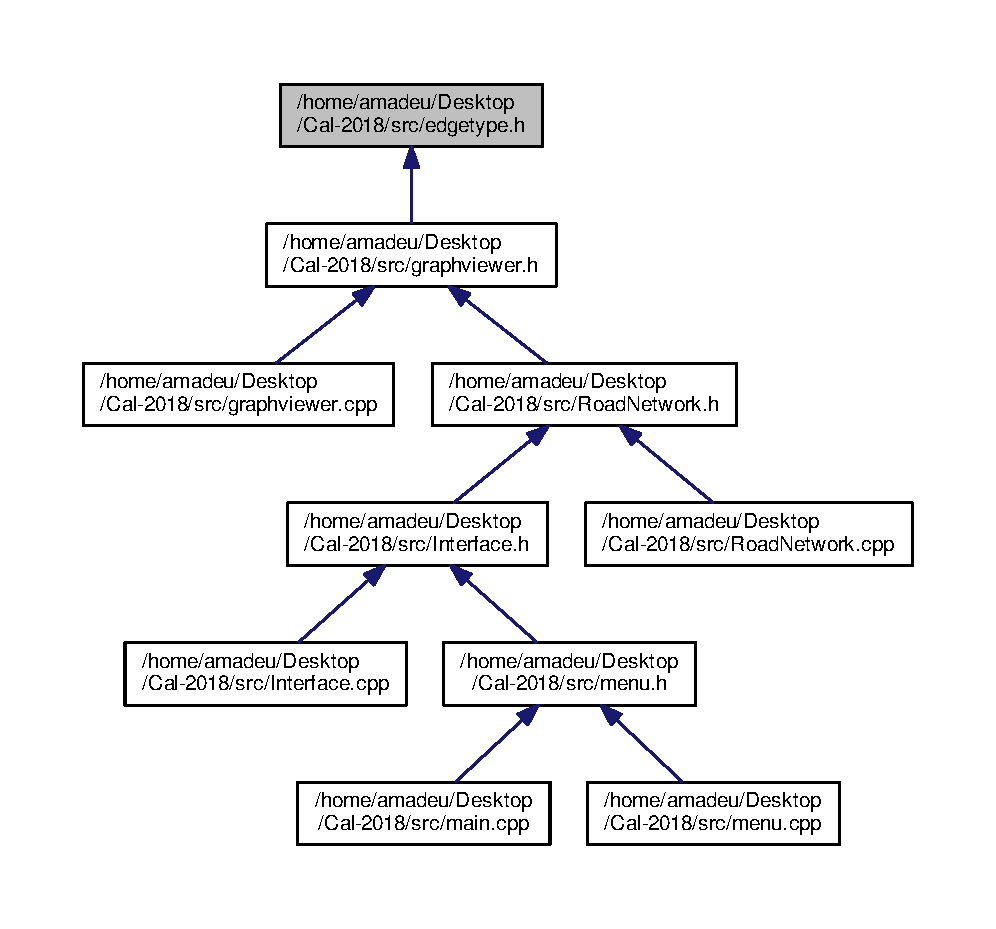
\includegraphics[width=350pt]{edgetype_8h__dep__incl}
\end{center}
\end{figure}
\subsection*{Classes}
\begin{DoxyCompactItemize}
\item 
class \hyperlink{classEdgeType}{Edge\+Type}
\end{DoxyCompactItemize}

\hypertarget{_graph_8h}{}\section{/\+Users/amadeuppereira/\+F\+E\+U\+P/2ano/\+Cal-\/2018/src/\+Graph.h File Reference}
\label{_graph_8h}\index{/\+Users/amadeuppereira/\+F\+E\+U\+P/2ano/\+Cal-\/2018/src/\+Graph.\+h@{/\+Users/amadeuppereira/\+F\+E\+U\+P/2ano/\+Cal-\/2018/src/\+Graph.\+h}}
{\ttfamily \#include $<$vector$>$}\newline
{\ttfamily \#include $<$queue$>$}\newline
{\ttfamily \#include $<$string$>$}\newline
{\ttfamily \#include $<$cmath$>$}\newline
{\ttfamily \#include $<$set$>$}\newline
{\ttfamily \#include $<$list$>$}\newline
{\ttfamily \#include $<$limits$>$}\newline
{\ttfamily \#include $<$climits$>$}\newline
{\ttfamily \#include \char`\"{}Mutable\+Priority\+Queue.\+h\char`\"{}}\newline
\subsection*{Classes}
\begin{DoxyCompactItemize}
\item 
class \mbox{\hyperlink{class_edge}{Edge$<$ T $>$}}
\item 
class \mbox{\hyperlink{class_graph}{Graph$<$ T $>$}}
\item 
class \mbox{\hyperlink{class_vertex}{Vertex$<$ T $>$}}
\item 
class \mbox{\hyperlink{class_carro}{Carro$<$ T $>$}}
\item 
class \mbox{\hyperlink{class_carro}{Carro$<$ T $>$}}
\item 
class \mbox{\hyperlink{class_vertex}{Vertex$<$ T $>$}}
\item 
struct \mbox{\hyperlink{structvertex__greater__than}{vertex\+\_\+greater\+\_\+than$<$ T $>$}}
\item 
class \mbox{\hyperlink{class_edge}{Edge$<$ T $>$}}
\item 
class \mbox{\hyperlink{class_graph}{Graph$<$ T $>$}}
\end{DoxyCompactItemize}
\subsection*{Macros}
\begin{DoxyCompactItemize}
\item 
\#define \mbox{\hyperlink{_graph_8h_a12c2040f25d8e3a7b9e1c2024c618cb6}{I\+NF}}~std\+::numeric\+\_\+limits$<$double$>$\+::max()
\item 
\#define \mbox{\hyperlink{_graph_8h_abc29155cbf8d3ba92a8cb487bbabdc66}{M\+A\+X\+\_\+\+C\+A\+P\+A\+C\+I\+TY}}~10
\end{DoxyCompactItemize}


\subsection{Macro Definition Documentation}
\mbox{\Hypertarget{_graph_8h_a12c2040f25d8e3a7b9e1c2024c618cb6}\label{_graph_8h_a12c2040f25d8e3a7b9e1c2024c618cb6}} 
\index{Graph.\+h@{Graph.\+h}!I\+NF@{I\+NF}}
\index{I\+NF@{I\+NF}!Graph.\+h@{Graph.\+h}}
\subsubsection{\texorpdfstring{I\+NF}{INF}}
{\footnotesize\ttfamily \#define I\+NF~std\+::numeric\+\_\+limits$<$double$>$\+::max()}

\mbox{\Hypertarget{_graph_8h_abc29155cbf8d3ba92a8cb487bbabdc66}\label{_graph_8h_abc29155cbf8d3ba92a8cb487bbabdc66}} 
\index{Graph.\+h@{Graph.\+h}!M\+A\+X\+\_\+\+C\+A\+P\+A\+C\+I\+TY@{M\+A\+X\+\_\+\+C\+A\+P\+A\+C\+I\+TY}}
\index{M\+A\+X\+\_\+\+C\+A\+P\+A\+C\+I\+TY@{M\+A\+X\+\_\+\+C\+A\+P\+A\+C\+I\+TY}!Graph.\+h@{Graph.\+h}}
\subsubsection{\texorpdfstring{M\+A\+X\+\_\+\+C\+A\+P\+A\+C\+I\+TY}{MAX\_CAPACITY}}
{\footnotesize\ttfamily \#define M\+A\+X\+\_\+\+C\+A\+P\+A\+C\+I\+TY~10}

Capacidade maxima das arestas 
\hypertarget{graphviewer_8cpp}{}\section{/\+Users/amadeuppereira/\+F\+E\+U\+P/2ano/\+Cal-\/2018/src/graphviewer.cpp File Reference}
\label{graphviewer_8cpp}\index{/\+Users/amadeuppereira/\+F\+E\+U\+P/2ano/\+Cal-\/2018/src/graphviewer.\+cpp@{/\+Users/amadeuppereira/\+F\+E\+U\+P/2ano/\+Cal-\/2018/src/graphviewer.\+cpp}}
{\ttfamily \#include \char`\"{}graphviewer.\+h\char`\"{}}\newline
{\ttfamily \#include $<$string$>$}\newline
{\ttfamily \#include $<$sstream$>$}\newline

\hypertarget{graphviewer_8h}{}\section{/home/amadeu/\+Desktop/\+Cal-\/2018/src/graphviewer.h File Reference}
\label{graphviewer_8h}\index{/home/amadeu/\+Desktop/\+Cal-\/2018/src/graphviewer.\+h@{/home/amadeu/\+Desktop/\+Cal-\/2018/src/graphviewer.\+h}}
{\ttfamily \#include $<$winsock2.\+h$>$}\\*
{\ttfamily \#include $<$Windows.\+h$>$}\\*
{\ttfamily \#include $<$stdlib.\+h$>$}\\*
{\ttfamily \#include $<$signal.\+h$>$}\\*
{\ttfamily \#include $<$string$>$}\\*
{\ttfamily \#include \char`\"{}edgetype.\+h\char`\"{}}\\*
{\ttfamily \#include \char`\"{}connection.\+h\char`\"{}}\\*
Include dependency graph for graphviewer.\+h\+:\nopagebreak
\begin{figure}[H]
\begin{center}
\leavevmode
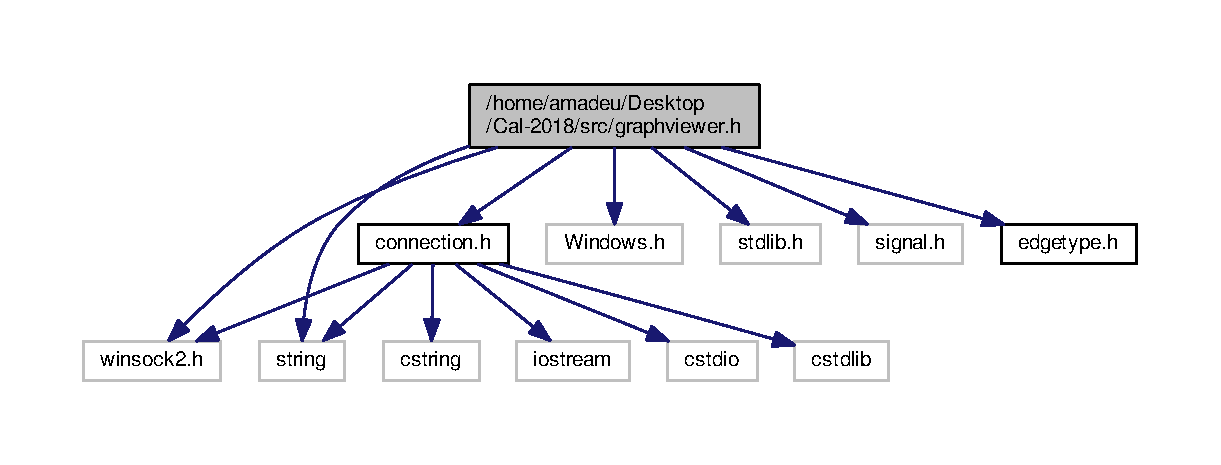
\includegraphics[width=350pt]{graphviewer_8h__incl}
\end{center}
\end{figure}
This graph shows which files directly or indirectly include this file\+:\nopagebreak
\begin{figure}[H]
\begin{center}
\leavevmode
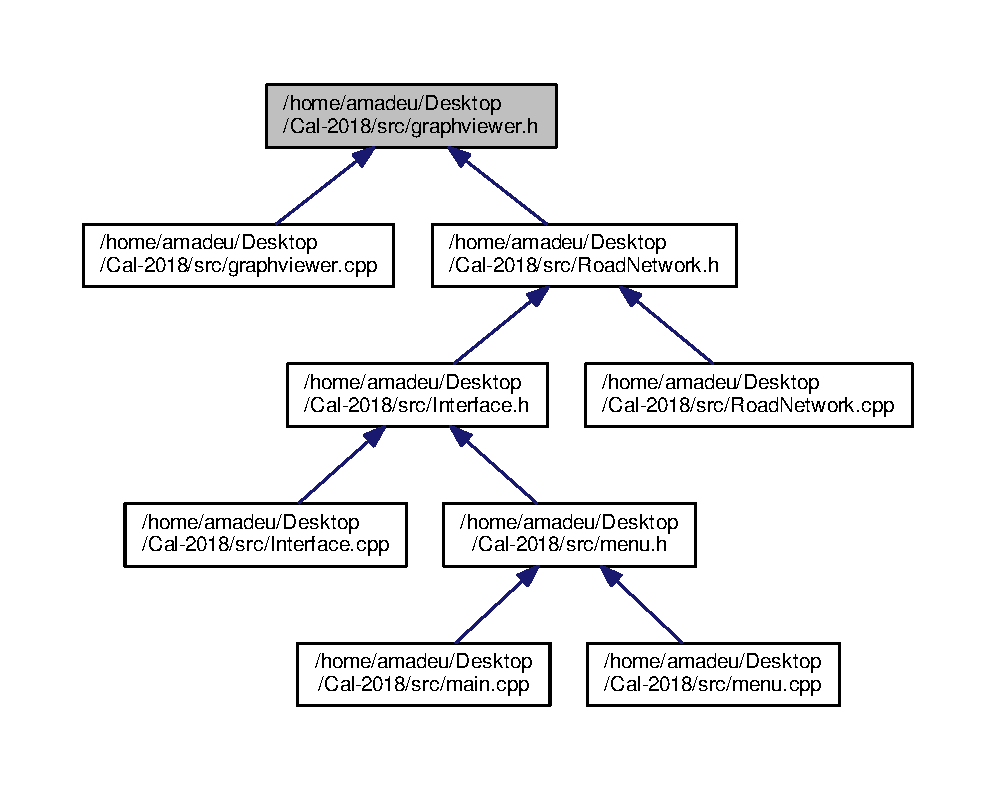
\includegraphics[width=350pt]{graphviewer_8h__dep__incl}
\end{center}
\end{figure}
\subsection*{Classes}
\begin{DoxyCompactItemize}
\item 
class \hyperlink{classGraphViewer}{Graph\+Viewer}
\end{DoxyCompactItemize}
\subsection*{Macros}
\begin{DoxyCompactItemize}
\item 
\#define \hyperlink{graphviewer_8h_a79d10e672abb49ad63eeaa8aaef57c38}{B\+L\+UE}~\char`\"{}B\+L\+UE\char`\"{}
\item 
\#define \hyperlink{graphviewer_8h_a8d23feea868a983c8c2b661e1e16972f}{R\+ED}~\char`\"{}R\+ED\char`\"{}
\item 
\#define \hyperlink{graphviewer_8h_ada419fe3b48fcf19daed7cc57ccf1174}{P\+I\+NK}~\char`\"{}P\+I\+NK\char`\"{}
\item 
\#define \hyperlink{graphviewer_8h_a7b3b25cba33b07c303f3060fe41887f6}{B\+L\+A\+CK}~\char`\"{}B\+L\+A\+CK\char`\"{}
\item 
\#define \hyperlink{graphviewer_8h_a87b537f5fa5c109d3c05c13d6b18f382}{W\+H\+I\+TE}~\char`\"{}W\+H\+I\+TE\char`\"{}
\item 
\#define \hyperlink{graphviewer_8h_ac5b6e19bf06822021f35602c59658de3}{O\+R\+A\+N\+GE}~\char`\"{}O\+R\+A\+N\+GE\char`\"{}
\item 
\#define \hyperlink{graphviewer_8h_abf681265909adf3d3e8116c93c0ba179}{Y\+E\+L\+L\+OW}~\char`\"{}Y\+E\+L\+L\+OW\char`\"{}
\item 
\#define \hyperlink{graphviewer_8h_acfbc006ea433ad708fdee3e82996e721}{G\+R\+E\+EN}~\char`\"{}G\+R\+E\+EN\char`\"{}
\item 
\#define \hyperlink{graphviewer_8h_ad243f93c16bc4c1d3e0a13b84421d760}{C\+Y\+AN}~\char`\"{}C\+Y\+AN\char`\"{}
\item 
\#define \hyperlink{graphviewer_8h_ae5f70677050eecd8909e0248e07b9e73}{G\+R\+AY}~\char`\"{}G\+R\+AY\char`\"{}
\item 
\#define \hyperlink{graphviewer_8h_aca56870f2285abae489635f0ee4d65e3}{D\+A\+R\+K\+\_\+\+G\+R\+AY}~\char`\"{}D\+A\+R\+K\+\_\+\+G\+R\+AY\char`\"{}
\item 
\#define \hyperlink{graphviewer_8h_a9663e02e20b5b578e6a31adae265cb88}{L\+I\+G\+H\+T\+\_\+\+G\+R\+AY}~\char`\"{}L\+I\+G\+H\+T\+\_\+\+G\+R\+AY\char`\"{}
\item 
\#define \hyperlink{graphviewer_8h_a6f699060902f800f12aaae150f3a708e}{M\+A\+G\+E\+N\+TA}~\char`\"{}M\+A\+G\+E\+N\+TA\char`\"{}
\end{DoxyCompactItemize}


\subsection{Macro Definition Documentation}
\index{graphviewer.\+h@{graphviewer.\+h}!B\+L\+A\+CK@{B\+L\+A\+CK}}
\index{B\+L\+A\+CK@{B\+L\+A\+CK}!graphviewer.\+h@{graphviewer.\+h}}
\subsubsection[{\texorpdfstring{B\+L\+A\+CK}{BLACK}}]{\setlength{\rightskip}{0pt plus 5cm}\#define B\+L\+A\+CK~\char`\"{}B\+L\+A\+CK\char`\"{}}\hypertarget{graphviewer_8h_a7b3b25cba33b07c303f3060fe41887f6}{}\label{graphviewer_8h_a7b3b25cba33b07c303f3060fe41887f6}
\index{graphviewer.\+h@{graphviewer.\+h}!B\+L\+UE@{B\+L\+UE}}
\index{B\+L\+UE@{B\+L\+UE}!graphviewer.\+h@{graphviewer.\+h}}
\subsubsection[{\texorpdfstring{B\+L\+UE}{BLUE}}]{\setlength{\rightskip}{0pt plus 5cm}\#define B\+L\+UE~\char`\"{}B\+L\+UE\char`\"{}}\hypertarget{graphviewer_8h_a79d10e672abb49ad63eeaa8aaef57c38}{}\label{graphviewer_8h_a79d10e672abb49ad63eeaa8aaef57c38}
\index{graphviewer.\+h@{graphviewer.\+h}!C\+Y\+AN@{C\+Y\+AN}}
\index{C\+Y\+AN@{C\+Y\+AN}!graphviewer.\+h@{graphviewer.\+h}}
\subsubsection[{\texorpdfstring{C\+Y\+AN}{CYAN}}]{\setlength{\rightskip}{0pt plus 5cm}\#define C\+Y\+AN~\char`\"{}C\+Y\+AN\char`\"{}}\hypertarget{graphviewer_8h_ad243f93c16bc4c1d3e0a13b84421d760}{}\label{graphviewer_8h_ad243f93c16bc4c1d3e0a13b84421d760}
\index{graphviewer.\+h@{graphviewer.\+h}!D\+A\+R\+K\+\_\+\+G\+R\+AY@{D\+A\+R\+K\+\_\+\+G\+R\+AY}}
\index{D\+A\+R\+K\+\_\+\+G\+R\+AY@{D\+A\+R\+K\+\_\+\+G\+R\+AY}!graphviewer.\+h@{graphviewer.\+h}}
\subsubsection[{\texorpdfstring{D\+A\+R\+K\+\_\+\+G\+R\+AY}{DARK_GRAY}}]{\setlength{\rightskip}{0pt plus 5cm}\#define D\+A\+R\+K\+\_\+\+G\+R\+AY~\char`\"{}D\+A\+R\+K\+\_\+\+G\+R\+AY\char`\"{}}\hypertarget{graphviewer_8h_aca56870f2285abae489635f0ee4d65e3}{}\label{graphviewer_8h_aca56870f2285abae489635f0ee4d65e3}
\index{graphviewer.\+h@{graphviewer.\+h}!G\+R\+AY@{G\+R\+AY}}
\index{G\+R\+AY@{G\+R\+AY}!graphviewer.\+h@{graphviewer.\+h}}
\subsubsection[{\texorpdfstring{G\+R\+AY}{GRAY}}]{\setlength{\rightskip}{0pt plus 5cm}\#define G\+R\+AY~\char`\"{}G\+R\+AY\char`\"{}}\hypertarget{graphviewer_8h_ae5f70677050eecd8909e0248e07b9e73}{}\label{graphviewer_8h_ae5f70677050eecd8909e0248e07b9e73}
\index{graphviewer.\+h@{graphviewer.\+h}!G\+R\+E\+EN@{G\+R\+E\+EN}}
\index{G\+R\+E\+EN@{G\+R\+E\+EN}!graphviewer.\+h@{graphviewer.\+h}}
\subsubsection[{\texorpdfstring{G\+R\+E\+EN}{GREEN}}]{\setlength{\rightskip}{0pt plus 5cm}\#define G\+R\+E\+EN~\char`\"{}G\+R\+E\+EN\char`\"{}}\hypertarget{graphviewer_8h_acfbc006ea433ad708fdee3e82996e721}{}\label{graphviewer_8h_acfbc006ea433ad708fdee3e82996e721}
\index{graphviewer.\+h@{graphviewer.\+h}!L\+I\+G\+H\+T\+\_\+\+G\+R\+AY@{L\+I\+G\+H\+T\+\_\+\+G\+R\+AY}}
\index{L\+I\+G\+H\+T\+\_\+\+G\+R\+AY@{L\+I\+G\+H\+T\+\_\+\+G\+R\+AY}!graphviewer.\+h@{graphviewer.\+h}}
\subsubsection[{\texorpdfstring{L\+I\+G\+H\+T\+\_\+\+G\+R\+AY}{LIGHT_GRAY}}]{\setlength{\rightskip}{0pt plus 5cm}\#define L\+I\+G\+H\+T\+\_\+\+G\+R\+AY~\char`\"{}L\+I\+G\+H\+T\+\_\+\+G\+R\+AY\char`\"{}}\hypertarget{graphviewer_8h_a9663e02e20b5b578e6a31adae265cb88}{}\label{graphviewer_8h_a9663e02e20b5b578e6a31adae265cb88}
\index{graphviewer.\+h@{graphviewer.\+h}!M\+A\+G\+E\+N\+TA@{M\+A\+G\+E\+N\+TA}}
\index{M\+A\+G\+E\+N\+TA@{M\+A\+G\+E\+N\+TA}!graphviewer.\+h@{graphviewer.\+h}}
\subsubsection[{\texorpdfstring{M\+A\+G\+E\+N\+TA}{MAGENTA}}]{\setlength{\rightskip}{0pt plus 5cm}\#define M\+A\+G\+E\+N\+TA~\char`\"{}M\+A\+G\+E\+N\+TA\char`\"{}}\hypertarget{graphviewer_8h_a6f699060902f800f12aaae150f3a708e}{}\label{graphviewer_8h_a6f699060902f800f12aaae150f3a708e}
\index{graphviewer.\+h@{graphviewer.\+h}!O\+R\+A\+N\+GE@{O\+R\+A\+N\+GE}}
\index{O\+R\+A\+N\+GE@{O\+R\+A\+N\+GE}!graphviewer.\+h@{graphviewer.\+h}}
\subsubsection[{\texorpdfstring{O\+R\+A\+N\+GE}{ORANGE}}]{\setlength{\rightskip}{0pt plus 5cm}\#define O\+R\+A\+N\+GE~\char`\"{}O\+R\+A\+N\+GE\char`\"{}}\hypertarget{graphviewer_8h_ac5b6e19bf06822021f35602c59658de3}{}\label{graphviewer_8h_ac5b6e19bf06822021f35602c59658de3}
\index{graphviewer.\+h@{graphviewer.\+h}!P\+I\+NK@{P\+I\+NK}}
\index{P\+I\+NK@{P\+I\+NK}!graphviewer.\+h@{graphviewer.\+h}}
\subsubsection[{\texorpdfstring{P\+I\+NK}{PINK}}]{\setlength{\rightskip}{0pt plus 5cm}\#define P\+I\+NK~\char`\"{}P\+I\+NK\char`\"{}}\hypertarget{graphviewer_8h_ada419fe3b48fcf19daed7cc57ccf1174}{}\label{graphviewer_8h_ada419fe3b48fcf19daed7cc57ccf1174}
\index{graphviewer.\+h@{graphviewer.\+h}!R\+ED@{R\+ED}}
\index{R\+ED@{R\+ED}!graphviewer.\+h@{graphviewer.\+h}}
\subsubsection[{\texorpdfstring{R\+ED}{RED}}]{\setlength{\rightskip}{0pt plus 5cm}\#define R\+ED~\char`\"{}R\+ED\char`\"{}}\hypertarget{graphviewer_8h_a8d23feea868a983c8c2b661e1e16972f}{}\label{graphviewer_8h_a8d23feea868a983c8c2b661e1e16972f}
\index{graphviewer.\+h@{graphviewer.\+h}!W\+H\+I\+TE@{W\+H\+I\+TE}}
\index{W\+H\+I\+TE@{W\+H\+I\+TE}!graphviewer.\+h@{graphviewer.\+h}}
\subsubsection[{\texorpdfstring{W\+H\+I\+TE}{WHITE}}]{\setlength{\rightskip}{0pt plus 5cm}\#define W\+H\+I\+TE~\char`\"{}W\+H\+I\+TE\char`\"{}}\hypertarget{graphviewer_8h_a87b537f5fa5c109d3c05c13d6b18f382}{}\label{graphviewer_8h_a87b537f5fa5c109d3c05c13d6b18f382}
\index{graphviewer.\+h@{graphviewer.\+h}!Y\+E\+L\+L\+OW@{Y\+E\+L\+L\+OW}}
\index{Y\+E\+L\+L\+OW@{Y\+E\+L\+L\+OW}!graphviewer.\+h@{graphviewer.\+h}}
\subsubsection[{\texorpdfstring{Y\+E\+L\+L\+OW}{YELLOW}}]{\setlength{\rightskip}{0pt plus 5cm}\#define Y\+E\+L\+L\+OW~\char`\"{}Y\+E\+L\+L\+OW\char`\"{}}\hypertarget{graphviewer_8h_abf681265909adf3d3e8116c93c0ba179}{}\label{graphviewer_8h_abf681265909adf3d3e8116c93c0ba179}

\hypertarget{_interface_8cpp}{}\section{/\+Users/amadeuppereira/\+F\+E\+U\+P/2ano/\+Cal-\/2018/src/\+Interface.cpp File Reference}
\label{_interface_8cpp}\index{/\+Users/amadeuppereira/\+F\+E\+U\+P/2ano/\+Cal-\/2018/src/\+Interface.\+cpp@{/\+Users/amadeuppereira/\+F\+E\+U\+P/2ano/\+Cal-\/2018/src/\+Interface.\+cpp}}
{\ttfamily \#include \char`\"{}Interface.\+h\char`\"{}}\newline

\hypertarget{_interface_8h}{}\section{/\+Users/amadeuppereira/\+F\+E\+U\+P/2ano/\+Cal-\/2018/src/\+Interface.h File Reference}
\label{_interface_8h}\index{/\+Users/amadeuppereira/\+F\+E\+U\+P/2ano/\+Cal-\/2018/src/\+Interface.\+h@{/\+Users/amadeuppereira/\+F\+E\+U\+P/2ano/\+Cal-\/2018/src/\+Interface.\+h}}
{\ttfamily \#include \char`\"{}Road\+Network.\+h\char`\"{}}\newline
{\ttfamily \#include $<$set$>$}\newline
{\ttfamily \#include $<$unistd.\+h$>$}\newline
\subsection*{Classes}
\begin{DoxyCompactItemize}
\item 
class \mbox{\hyperlink{class_interface}{Interface}}
\end{DoxyCompactItemize}

\hypertarget{main_8cpp}{}\section{/home/amadeu/\+Desktop/\+Cal-\/2018/src/main.cpp File Reference}
\label{main_8cpp}\index{/home/amadeu/\+Desktop/\+Cal-\/2018/src/main.\+cpp@{/home/amadeu/\+Desktop/\+Cal-\/2018/src/main.\+cpp}}
{\ttfamily \#include $<$iostream$>$}\\*
{\ttfamily \#include $<$string$>$}\\*
{\ttfamily \#include \char`\"{}menu.\+h\char`\"{}}\\*
Include dependency graph for main.\+cpp\+:\nopagebreak
\begin{figure}[H]
\begin{center}
\leavevmode
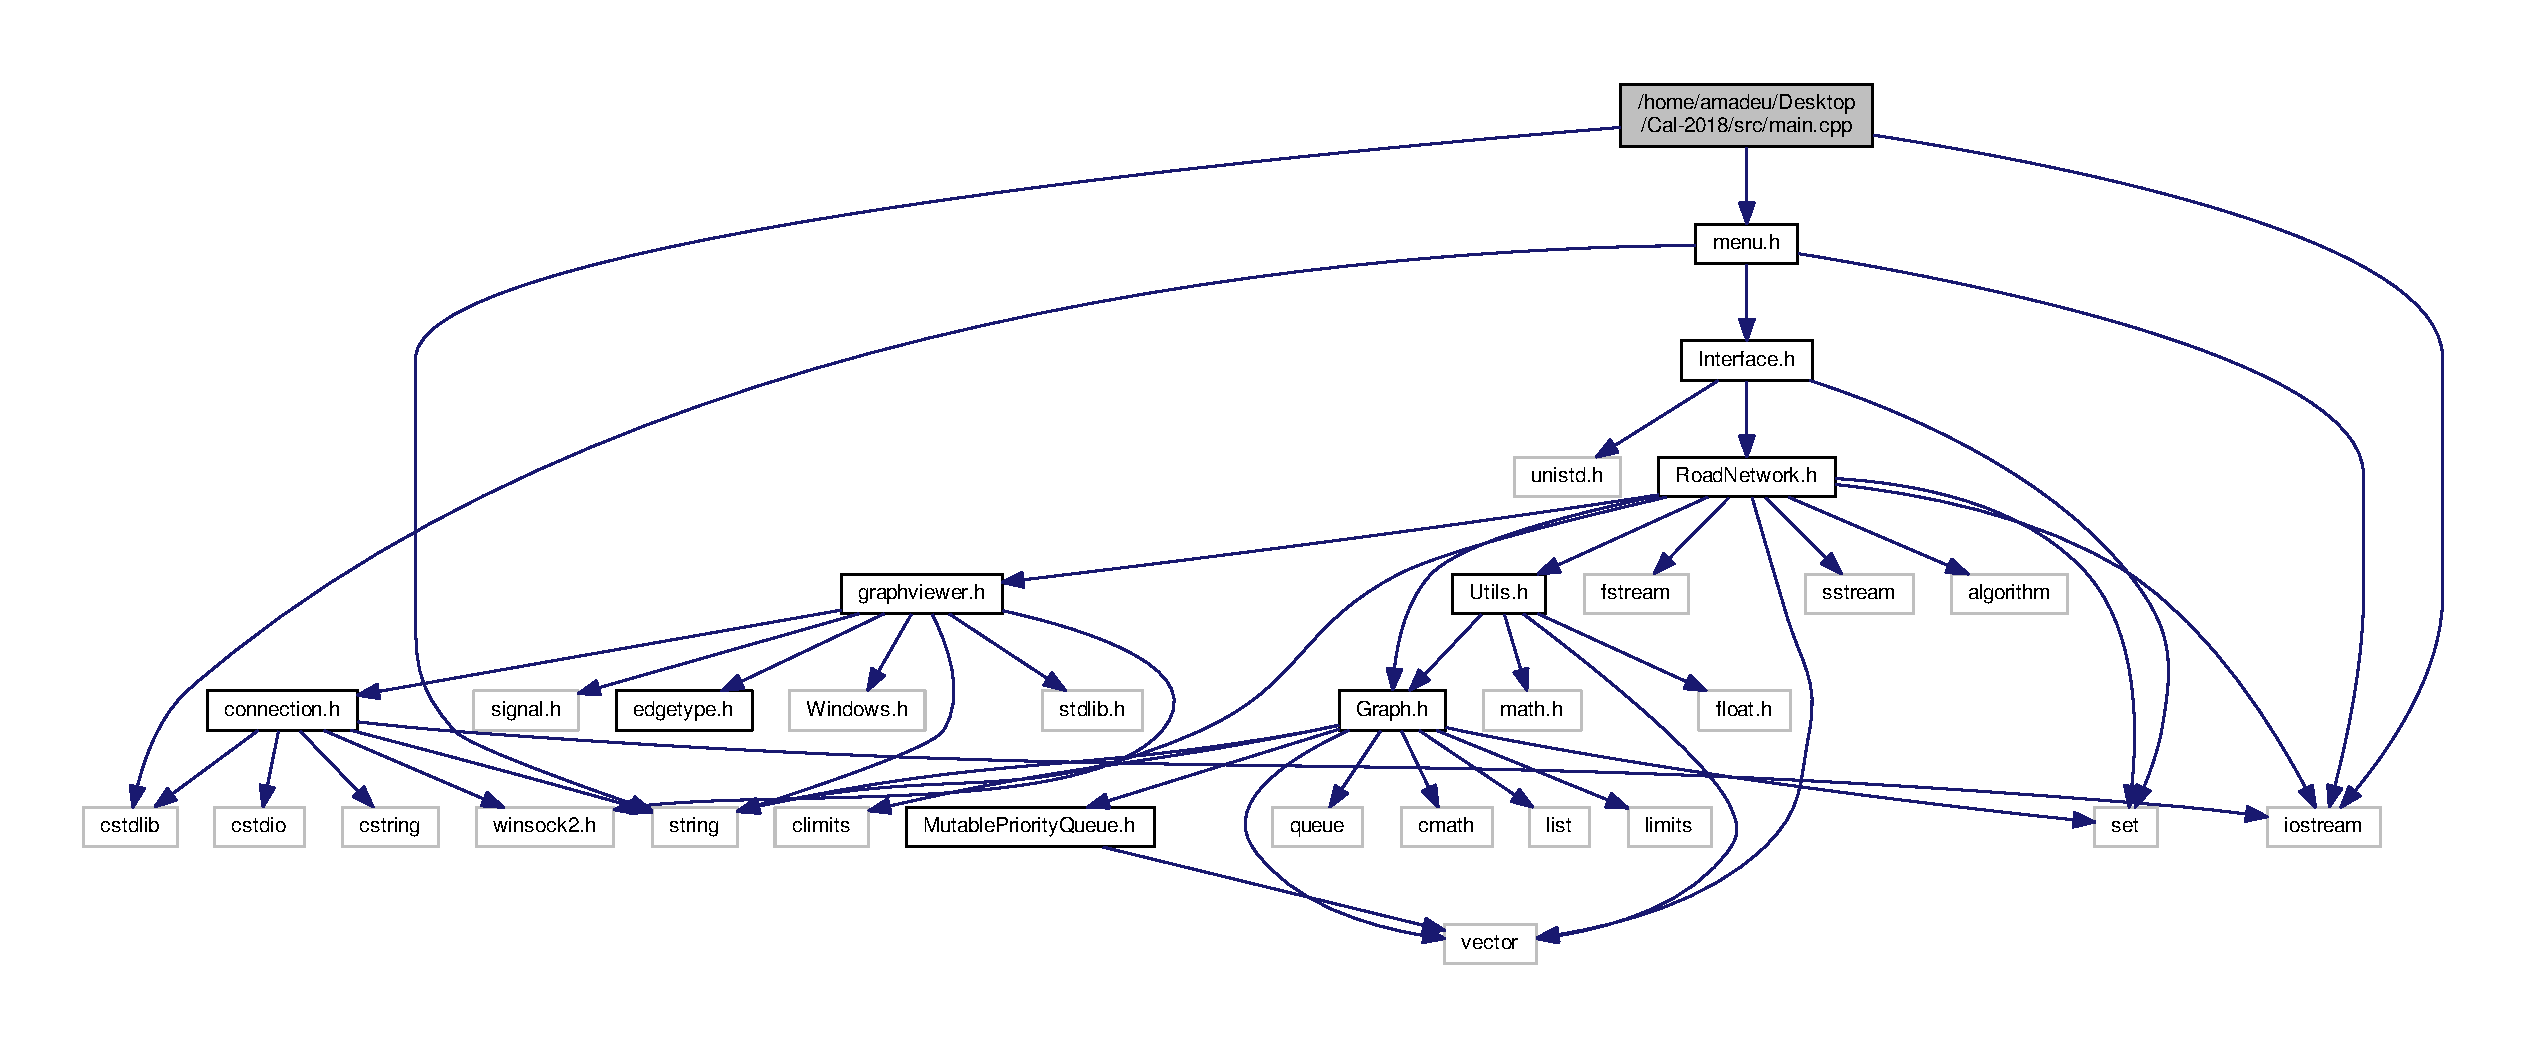
\includegraphics[width=350pt]{main_8cpp__incl}
\end{center}
\end{figure}
\subsection*{Functions}
\begin{DoxyCompactItemize}
\item 
int \hyperlink{main_8cpp_ae66f6b31b5ad750f1fe042a706a4e3d4}{main} ()
\end{DoxyCompactItemize}


\subsection{Function Documentation}
\index{main.\+cpp@{main.\+cpp}!main@{main}}
\index{main@{main}!main.\+cpp@{main.\+cpp}}
\subsubsection[{\texorpdfstring{main()}{main()}}]{\setlength{\rightskip}{0pt plus 5cm}int main (
\begin{DoxyParamCaption}
{}
\end{DoxyParamCaption}
)}\hypertarget{main_8cpp_ae66f6b31b5ad750f1fe042a706a4e3d4}{}\label{main_8cpp_ae66f6b31b5ad750f1fe042a706a4e3d4}

\hypertarget{menu_8cpp}{}\section{/home/amadeu/\+Desktop/\+Cal-\/2018/src/menu.cpp File Reference}
\label{menu_8cpp}\index{/home/amadeu/\+Desktop/\+Cal-\/2018/src/menu.\+cpp@{/home/amadeu/\+Desktop/\+Cal-\/2018/src/menu.\+cpp}}
{\ttfamily \#include \char`\"{}menu.\+h\char`\"{}}\\*
Include dependency graph for menu.\+cpp\+:\nopagebreak
\begin{figure}[H]
\begin{center}
\leavevmode
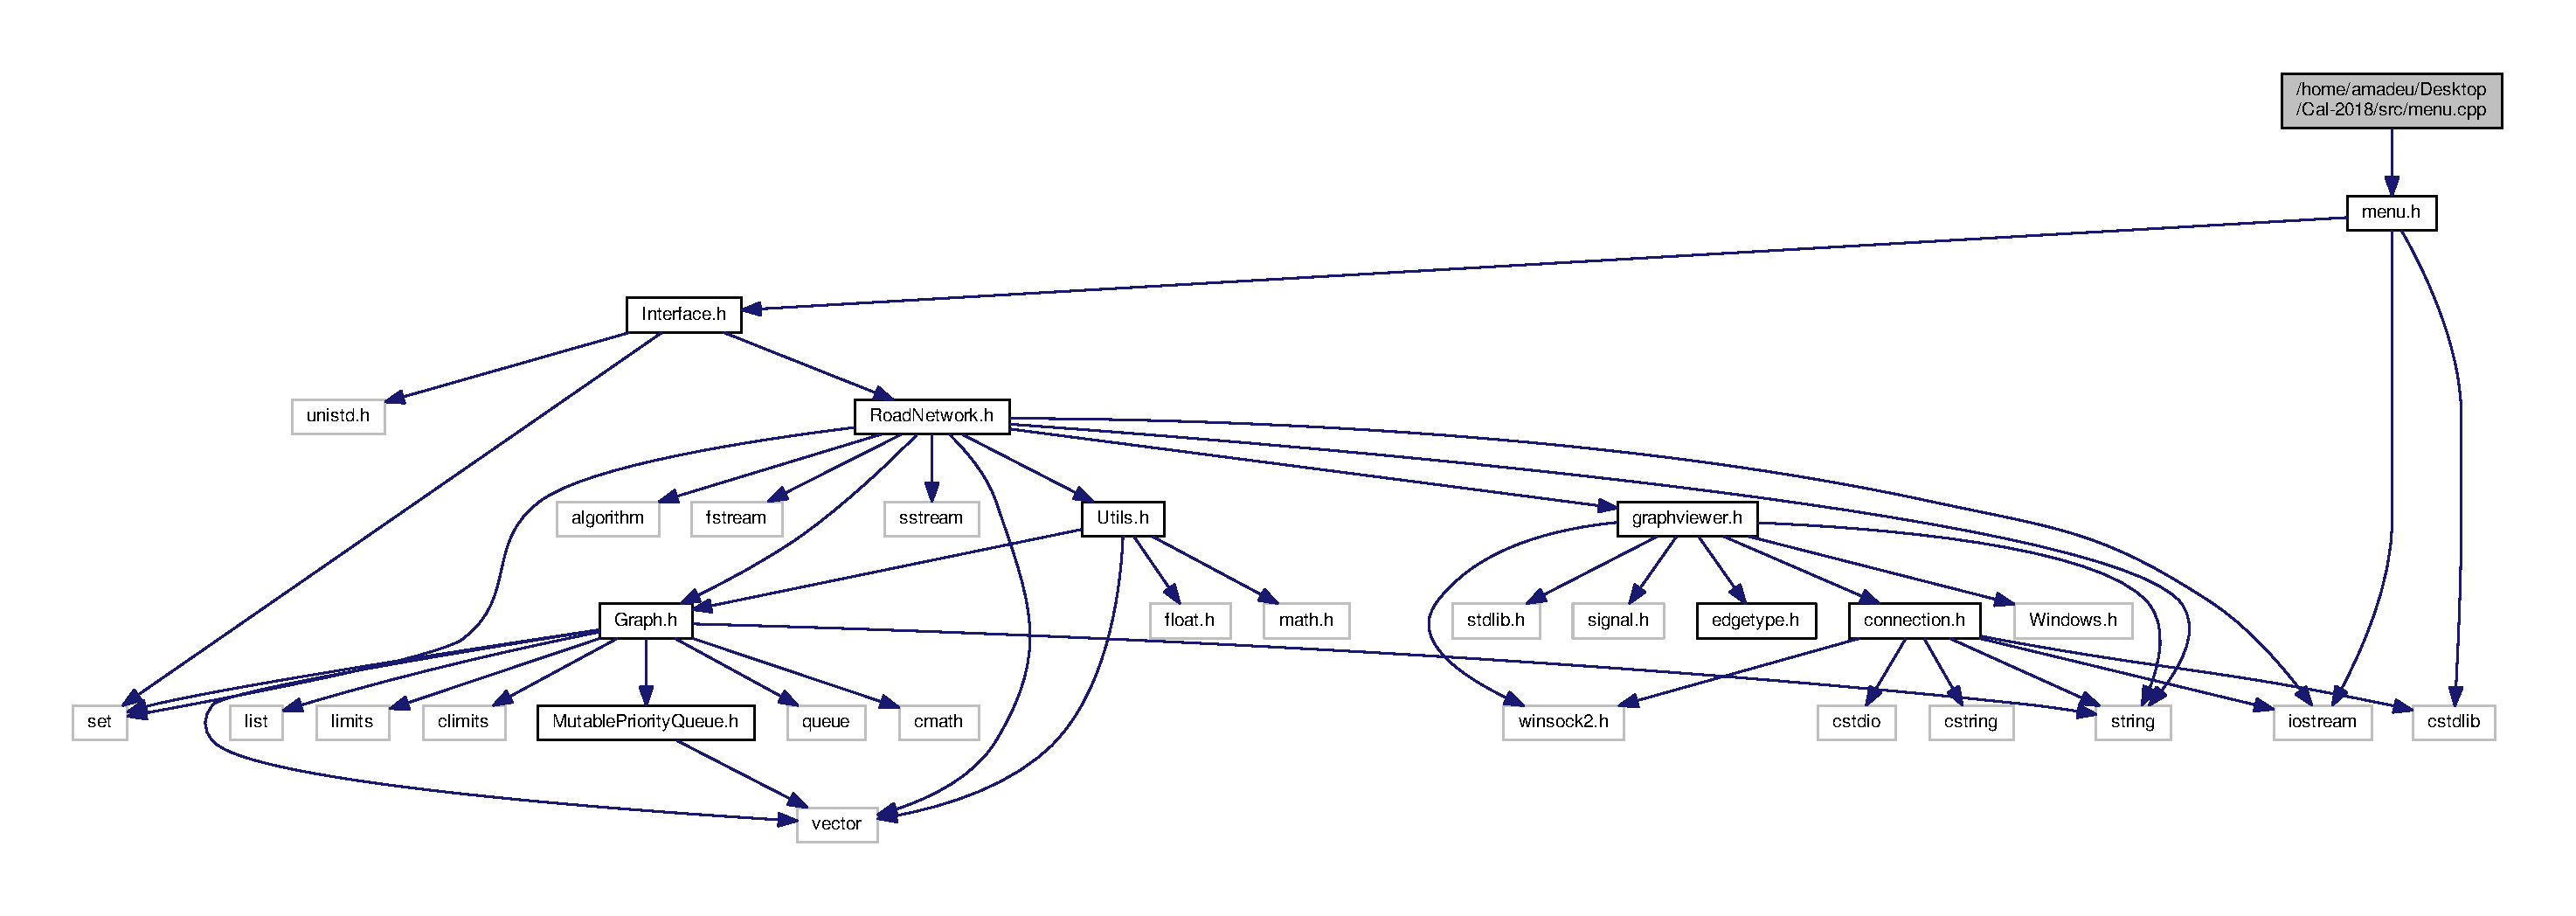
\includegraphics[width=350pt]{menu_8cpp__incl}
\end{center}
\end{figure}
\subsection*{Functions}
\begin{DoxyCompactItemize}
\item 
void \hyperlink{menu_8cpp_ae3e62f59c2eb3d57ecc15606da4a7c20}{save\+Files} ()
\item 
void \hyperlink{menu_8cpp_a2a0e843767aeea4f433a28b9c54f573a}{menu} ()
\end{DoxyCompactItemize}
\subsection*{Variables}
\begin{DoxyCompactItemize}
\item 
static \hyperlink{classInterface}{Interface} \hyperlink{menu_8cpp_a98862a04b438a5359a542f245ca97b62}{i} = \hyperlink{classInterface}{Interface}()
\end{DoxyCompactItemize}


\subsection{Function Documentation}
\index{menu.\+cpp@{menu.\+cpp}!menu@{menu}}
\index{menu@{menu}!menu.\+cpp@{menu.\+cpp}}
\subsubsection[{\texorpdfstring{menu()}{menu()}}]{\setlength{\rightskip}{0pt plus 5cm}void menu (
\begin{DoxyParamCaption}
{}
\end{DoxyParamCaption}
)}\hypertarget{menu_8cpp_a2a0e843767aeea4f433a28b9c54f573a}{}\label{menu_8cpp_a2a0e843767aeea4f433a28b9c54f573a}
Menu do programa \index{menu.\+cpp@{menu.\+cpp}!save\+Files@{save\+Files}}
\index{save\+Files@{save\+Files}!menu.\+cpp@{menu.\+cpp}}
\subsubsection[{\texorpdfstring{save\+Files()}{saveFiles()}}]{\setlength{\rightskip}{0pt plus 5cm}void save\+Files (
\begin{DoxyParamCaption}
{}
\end{DoxyParamCaption}
)}\hypertarget{menu_8cpp_ae3e62f59c2eb3d57ecc15606da4a7c20}{}\label{menu_8cpp_ae3e62f59c2eb3d57ecc15606da4a7c20}


\subsection{Variable Documentation}
\index{menu.\+cpp@{menu.\+cpp}!i@{i}}
\index{i@{i}!menu.\+cpp@{menu.\+cpp}}
\subsubsection[{\texorpdfstring{i}{i}}]{\setlength{\rightskip}{0pt plus 5cm}{\bf Interface} i = {\bf Interface}()\hspace{0.3cm}{\ttfamily [static]}}\hypertarget{menu_8cpp_a98862a04b438a5359a542f245ca97b62}{}\label{menu_8cpp_a98862a04b438a5359a542f245ca97b62}

\hypertarget{menu_8h}{}\section{/home/amadeu/\+Desktop/\+Cal-\/2018/src/menu.h File Reference}
\label{menu_8h}\index{/home/amadeu/\+Desktop/\+Cal-\/2018/src/menu.\+h@{/home/amadeu/\+Desktop/\+Cal-\/2018/src/menu.\+h}}
{\ttfamily \#include $<$iostream$>$}\\*
{\ttfamily \#include $<$cstdlib$>$}\\*
{\ttfamily \#include \char`\"{}Interface.\+h\char`\"{}}\\*
Include dependency graph for menu.\+h\+:\nopagebreak
\begin{figure}[H]
\begin{center}
\leavevmode
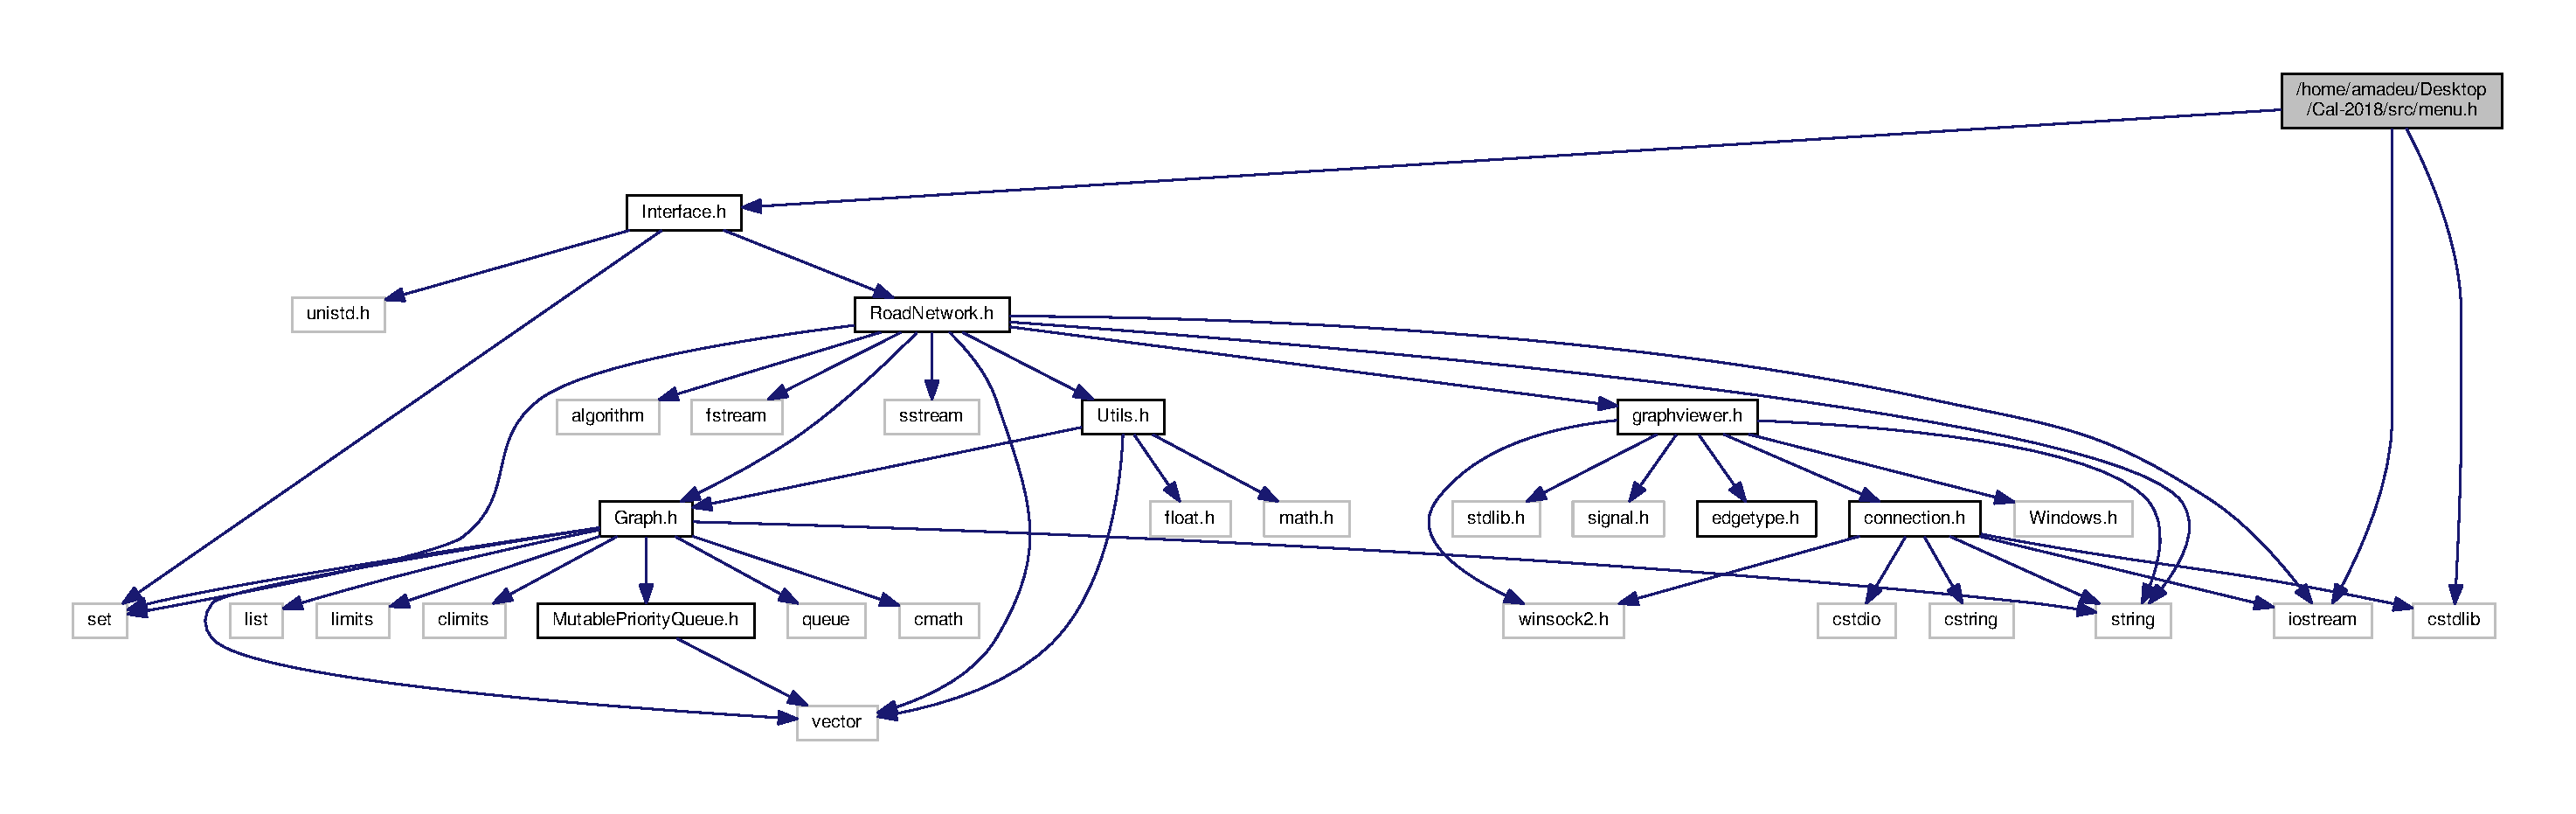
\includegraphics[width=350pt]{menu_8h__incl}
\end{center}
\end{figure}
This graph shows which files directly or indirectly include this file\+:\nopagebreak
\begin{figure}[H]
\begin{center}
\leavevmode
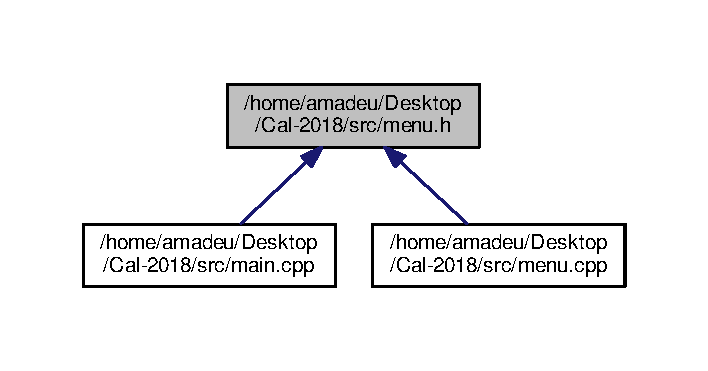
\includegraphics[width=340pt]{menu_8h__dep__incl}
\end{center}
\end{figure}
\subsection*{Functions}
\begin{DoxyCompactItemize}
\item 
void \hyperlink{menu_8h_a2a0e843767aeea4f433a28b9c54f573a}{menu} ()
\end{DoxyCompactItemize}


\subsection{Function Documentation}
\index{menu.\+h@{menu.\+h}!menu@{menu}}
\index{menu@{menu}!menu.\+h@{menu.\+h}}
\subsubsection[{\texorpdfstring{menu()}{menu()}}]{\setlength{\rightskip}{0pt plus 5cm}void menu (
\begin{DoxyParamCaption}
{}
\end{DoxyParamCaption}
)}\hypertarget{menu_8h_a2a0e843767aeea4f433a28b9c54f573a}{}\label{menu_8h_a2a0e843767aeea4f433a28b9c54f573a}
Menu do programa 
\hypertarget{_mutable_priority_queue_8h}{}\section{/\+Users/amadeuppereira/\+F\+E\+U\+P/2ano/\+Cal-\/2018/src/\+Mutable\+Priority\+Queue.h File Reference}
\label{_mutable_priority_queue_8h}\index{/\+Users/amadeuppereira/\+F\+E\+U\+P/2ano/\+Cal-\/2018/src/\+Mutable\+Priority\+Queue.\+h@{/\+Users/amadeuppereira/\+F\+E\+U\+P/2ano/\+Cal-\/2018/src/\+Mutable\+Priority\+Queue.\+h}}
{\ttfamily \#include $<$vector$>$}\newline
\subsection*{Classes}
\begin{DoxyCompactItemize}
\item 
class \mbox{\hyperlink{class_mutable_priority_queue}{Mutable\+Priority\+Queue$<$ T $>$}}
\end{DoxyCompactItemize}
\subsection*{Macros}
\begin{DoxyCompactItemize}
\item 
\#define \mbox{\hyperlink{_mutable_priority_queue_8h_a915a9564b15f2c25e828da2e9a05769c}{parent}}(\mbox{\hyperlink{menu_8cpp_a98862a04b438a5359a542f245ca97b62}{i}})~((\mbox{\hyperlink{menu_8cpp_a98862a04b438a5359a542f245ca97b62}{i}}) $>$$>$ 1)  /$\ast$ \mbox{\hyperlink{menu_8cpp_a98862a04b438a5359a542f245ca97b62}{i}} / 2 $\ast$/
\item 
\#define \mbox{\hyperlink{_mutable_priority_queue_8h_ac84ef3998ba958fd8abf03d08cc5ffcb}{left\+Child}}(\mbox{\hyperlink{menu_8cpp_a98862a04b438a5359a542f245ca97b62}{i}})~((\mbox{\hyperlink{menu_8cpp_a98862a04b438a5359a542f245ca97b62}{i}}) $<$$<$ 1)  /$\ast$ \mbox{\hyperlink{menu_8cpp_a98862a04b438a5359a542f245ca97b62}{i}} $\ast$ 2 $\ast$/
\end{DoxyCompactItemize}


\subsection{Macro Definition Documentation}
\mbox{\Hypertarget{_mutable_priority_queue_8h_ac84ef3998ba958fd8abf03d08cc5ffcb}\label{_mutable_priority_queue_8h_ac84ef3998ba958fd8abf03d08cc5ffcb}} 
\index{Mutable\+Priority\+Queue.\+h@{Mutable\+Priority\+Queue.\+h}!left\+Child@{left\+Child}}
\index{left\+Child@{left\+Child}!Mutable\+Priority\+Queue.\+h@{Mutable\+Priority\+Queue.\+h}}
\subsubsection{\texorpdfstring{left\+Child}{leftChild}}
{\footnotesize\ttfamily \#define left\+Child(\begin{DoxyParamCaption}\item[{}]{\mbox{\hyperlink{menu_8cpp_a98862a04b438a5359a542f245ca97b62}{i}} }\end{DoxyParamCaption})~((\mbox{\hyperlink{menu_8cpp_a98862a04b438a5359a542f245ca97b62}{i}}) $<$$<$ 1)  /$\ast$ \mbox{\hyperlink{menu_8cpp_a98862a04b438a5359a542f245ca97b62}{i}} $\ast$ 2 $\ast$/}

\mbox{\Hypertarget{_mutable_priority_queue_8h_a915a9564b15f2c25e828da2e9a05769c}\label{_mutable_priority_queue_8h_a915a9564b15f2c25e828da2e9a05769c}} 
\index{Mutable\+Priority\+Queue.\+h@{Mutable\+Priority\+Queue.\+h}!parent@{parent}}
\index{parent@{parent}!Mutable\+Priority\+Queue.\+h@{Mutable\+Priority\+Queue.\+h}}
\subsubsection{\texorpdfstring{parent}{parent}}
{\footnotesize\ttfamily \#define parent(\begin{DoxyParamCaption}\item[{}]{\mbox{\hyperlink{menu_8cpp_a98862a04b438a5359a542f245ca97b62}{i}} }\end{DoxyParamCaption})~((\mbox{\hyperlink{menu_8cpp_a98862a04b438a5359a542f245ca97b62}{i}}) $>$$>$ 1)  /$\ast$ \mbox{\hyperlink{menu_8cpp_a98862a04b438a5359a542f245ca97b62}{i}} / 2 $\ast$/}


\hypertarget{_road_network_8cpp}{}\section{/\+Users/amadeuppereira/\+F\+E\+U\+P/2ano/\+Cal-\/2018/src/\+Road\+Network.cpp File Reference}
\label{_road_network_8cpp}\index{/\+Users/amadeuppereira/\+F\+E\+U\+P/2ano/\+Cal-\/2018/src/\+Road\+Network.\+cpp@{/\+Users/amadeuppereira/\+F\+E\+U\+P/2ano/\+Cal-\/2018/src/\+Road\+Network.\+cpp}}
{\ttfamily \#include \char`\"{}Road\+Network.\+h\char`\"{}}\newline
\subsection*{Functions}
\begin{DoxyCompactItemize}
\item 
bool \mbox{\hyperlink{_road_network_8cpp_a76a4ba4ef25d3eb62249d90a3d128bc5}{compare\+Vector\+Edges}} (\mbox{\hyperlink{class_edge}{Edge}}$<$ int $>$ $\ast$edge1, \mbox{\hyperlink{class_edge}{Edge}}$<$ int $>$ $\ast$edge2)
\end{DoxyCompactItemize}
\subsection*{Variables}
\begin{DoxyCompactItemize}
\item 
const unsigned int \mbox{\hyperlink{_road_network_8cpp_a4ca038c853912ffb3a37812e88b871f2}{cost\+\_\+del}} = 1
\item 
const unsigned int \mbox{\hyperlink{_road_network_8cpp_ae4b61303f994910b5f5db03e4ff9f99e}{cost\+\_\+ins}} = 1
\item 
const unsigned int \mbox{\hyperlink{_road_network_8cpp_aedb9f422142e9db421225b6e51fead5f}{cost\+\_\+sub}} = 1
\end{DoxyCompactItemize}


\subsection{Function Documentation}
\mbox{\Hypertarget{_road_network_8cpp_a76a4ba4ef25d3eb62249d90a3d128bc5}\label{_road_network_8cpp_a76a4ba4ef25d3eb62249d90a3d128bc5}} 
\index{Road\+Network.\+cpp@{Road\+Network.\+cpp}!compare\+Vector\+Edges@{compare\+Vector\+Edges}}
\index{compare\+Vector\+Edges@{compare\+Vector\+Edges}!Road\+Network.\+cpp@{Road\+Network.\+cpp}}
\subsubsection{\texorpdfstring{compare\+Vector\+Edges()}{compareVectorEdges()}}
{\footnotesize\ttfamily bool compare\+Vector\+Edges (\begin{DoxyParamCaption}\item[{\mbox{\hyperlink{class_edge}{Edge}}$<$ int $>$ $\ast$}]{edge1,  }\item[{\mbox{\hyperlink{class_edge}{Edge}}$<$ int $>$ $\ast$}]{edge2 }\end{DoxyParamCaption})}



\subsection{Variable Documentation}
\mbox{\Hypertarget{_road_network_8cpp_a4ca038c853912ffb3a37812e88b871f2}\label{_road_network_8cpp_a4ca038c853912ffb3a37812e88b871f2}} 
\index{Road\+Network.\+cpp@{Road\+Network.\+cpp}!cost\+\_\+del@{cost\+\_\+del}}
\index{cost\+\_\+del@{cost\+\_\+del}!Road\+Network.\+cpp@{Road\+Network.\+cpp}}
\subsubsection{\texorpdfstring{cost\+\_\+del}{cost\_del}}
{\footnotesize\ttfamily const unsigned int cost\+\_\+del = 1}

\mbox{\Hypertarget{_road_network_8cpp_ae4b61303f994910b5f5db03e4ff9f99e}\label{_road_network_8cpp_ae4b61303f994910b5f5db03e4ff9f99e}} 
\index{Road\+Network.\+cpp@{Road\+Network.\+cpp}!cost\+\_\+ins@{cost\+\_\+ins}}
\index{cost\+\_\+ins@{cost\+\_\+ins}!Road\+Network.\+cpp@{Road\+Network.\+cpp}}
\subsubsection{\texorpdfstring{cost\+\_\+ins}{cost\_ins}}
{\footnotesize\ttfamily const unsigned int cost\+\_\+ins = 1}

\mbox{\Hypertarget{_road_network_8cpp_aedb9f422142e9db421225b6e51fead5f}\label{_road_network_8cpp_aedb9f422142e9db421225b6e51fead5f}} 
\index{Road\+Network.\+cpp@{Road\+Network.\+cpp}!cost\+\_\+sub@{cost\+\_\+sub}}
\index{cost\+\_\+sub@{cost\+\_\+sub}!Road\+Network.\+cpp@{Road\+Network.\+cpp}}
\subsubsection{\texorpdfstring{cost\+\_\+sub}{cost\_sub}}
{\footnotesize\ttfamily const unsigned int cost\+\_\+sub = 1}


\hypertarget{_road_network_8h}{}\section{/\+Users/amadeuppereira/\+F\+E\+U\+P/2ano/\+Cal-\/2018/src/\+Road\+Network.h File Reference}
\label{_road_network_8h}\index{/\+Users/amadeuppereira/\+F\+E\+U\+P/2ano/\+Cal-\/2018/src/\+Road\+Network.\+h@{/\+Users/amadeuppereira/\+F\+E\+U\+P/2ano/\+Cal-\/2018/src/\+Road\+Network.\+h}}
{\ttfamily \#include $<$iostream$>$}\newline
{\ttfamily \#include $<$fstream$>$}\newline
{\ttfamily \#include $<$sstream$>$}\newline
{\ttfamily \#include $<$string$>$}\newline
{\ttfamily \#include $<$algorithm$>$}\newline
{\ttfamily \#include $<$vector$>$}\newline
{\ttfamily \#include $<$set$>$}\newline
{\ttfamily \#include \char`\"{}Graph.\+h\char`\"{}}\newline
{\ttfamily \#include \char`\"{}graphviewer.\+h\char`\"{}}\newline
{\ttfamily \#include \char`\"{}Utils.\+h\char`\"{}}\newline
\subsection*{Classes}
\begin{DoxyCompactItemize}
\item 
class \mbox{\hyperlink{class_road_network}{Road\+Network}}
\end{DoxyCompactItemize}
\subsection*{Macros}
\begin{DoxyCompactItemize}
\item 
\#define \mbox{\hyperlink{_road_network_8h_a6e6e0f0a07b275692baea5c5ea99ae45}{D\+E\+F\+A\+U\+L\+T\+\_\+\+V\+E\+R\+T\+E\+X\+\_\+\+C\+O\+L\+OR}}~\char`\"{}blue\char`\"{}
\item 
\#define \mbox{\hyperlink{_road_network_8h_afc7c125091ba180d90d5c7aa19645d38}{D\+E\+F\+A\+U\+L\+T\+\_\+\+E\+D\+G\+E\+\_\+\+C\+O\+L\+OR}}~\char`\"{}green\char`\"{}
\item 
\#define \mbox{\hyperlink{_road_network_8h_a5d57b679ed7a8e206acb4b2e86534120}{H\+I\+G\+H\+L\+I\+G\+H\+T\+E\+D\+\_\+\+V\+E\+R\+T\+E\+X\+\_\+\+C\+O\+L\+OR}}~\char`\"{}yellow\char`\"{}
\item 
\#define \mbox{\hyperlink{_road_network_8h_a973c5f767642717d927a10c4ba7b0536}{H\+I\+G\+H\+L\+I\+G\+H\+T\+E\+D\+\_\+\+E\+D\+G\+E\+\_\+\+C\+O\+L\+OR}}~\char`\"{}yellow\char`\"{}
\item 
\#define \mbox{\hyperlink{_road_network_8h_aab9747c5846f722e12157db553d5fbaa}{M\+E\+D\+I\+U\+M\+\_\+\+T\+R\+A\+F\+F\+IC}}~\char`\"{}orange\char`\"{}
\item 
\#define \mbox{\hyperlink{_road_network_8h_a88ca92279b5d6c46600c7bbec05cd421}{H\+I\+G\+H\+\_\+\+T\+R\+A\+F\+F\+IC}}~\char`\"{}red\char`\"{}
\item 
\#define \mbox{\hyperlink{_road_network_8h_a85f4a39e351bd60a328dd9cf8cc4dae0}{B\+L\+O\+C\+K\+E\+D\+\_\+\+E\+D\+G\+E\+\_\+\+C\+O\+L\+OR}}~\char`\"{}black\char`\"{}
\end{DoxyCompactItemize}


\subsection{Macro Definition Documentation}
\mbox{\Hypertarget{_road_network_8h_a85f4a39e351bd60a328dd9cf8cc4dae0}\label{_road_network_8h_a85f4a39e351bd60a328dd9cf8cc4dae0}} 
\index{Road\+Network.\+h@{Road\+Network.\+h}!B\+L\+O\+C\+K\+E\+D\+\_\+\+E\+D\+G\+E\+\_\+\+C\+O\+L\+OR@{B\+L\+O\+C\+K\+E\+D\+\_\+\+E\+D\+G\+E\+\_\+\+C\+O\+L\+OR}}
\index{B\+L\+O\+C\+K\+E\+D\+\_\+\+E\+D\+G\+E\+\_\+\+C\+O\+L\+OR@{B\+L\+O\+C\+K\+E\+D\+\_\+\+E\+D\+G\+E\+\_\+\+C\+O\+L\+OR}!Road\+Network.\+h@{Road\+Network.\+h}}
\subsubsection{\texorpdfstring{B\+L\+O\+C\+K\+E\+D\+\_\+\+E\+D\+G\+E\+\_\+\+C\+O\+L\+OR}{BLOCKED\_EDGE\_COLOR}}
{\footnotesize\ttfamily \#define B\+L\+O\+C\+K\+E\+D\+\_\+\+E\+D\+G\+E\+\_\+\+C\+O\+L\+OR~\char`\"{}black\char`\"{}}

Cor das edges bloqueadas \mbox{\Hypertarget{_road_network_8h_afc7c125091ba180d90d5c7aa19645d38}\label{_road_network_8h_afc7c125091ba180d90d5c7aa19645d38}} 
\index{Road\+Network.\+h@{Road\+Network.\+h}!D\+E\+F\+A\+U\+L\+T\+\_\+\+E\+D\+G\+E\+\_\+\+C\+O\+L\+OR@{D\+E\+F\+A\+U\+L\+T\+\_\+\+E\+D\+G\+E\+\_\+\+C\+O\+L\+OR}}
\index{D\+E\+F\+A\+U\+L\+T\+\_\+\+E\+D\+G\+E\+\_\+\+C\+O\+L\+OR@{D\+E\+F\+A\+U\+L\+T\+\_\+\+E\+D\+G\+E\+\_\+\+C\+O\+L\+OR}!Road\+Network.\+h@{Road\+Network.\+h}}
\subsubsection{\texorpdfstring{D\+E\+F\+A\+U\+L\+T\+\_\+\+E\+D\+G\+E\+\_\+\+C\+O\+L\+OR}{DEFAULT\_EDGE\_COLOR}}
{\footnotesize\ttfamily \#define D\+E\+F\+A\+U\+L\+T\+\_\+\+E\+D\+G\+E\+\_\+\+C\+O\+L\+OR~\char`\"{}green\char`\"{}}

Cor das edges com pouco transito \mbox{\Hypertarget{_road_network_8h_a6e6e0f0a07b275692baea5c5ea99ae45}\label{_road_network_8h_a6e6e0f0a07b275692baea5c5ea99ae45}} 
\index{Road\+Network.\+h@{Road\+Network.\+h}!D\+E\+F\+A\+U\+L\+T\+\_\+\+V\+E\+R\+T\+E\+X\+\_\+\+C\+O\+L\+OR@{D\+E\+F\+A\+U\+L\+T\+\_\+\+V\+E\+R\+T\+E\+X\+\_\+\+C\+O\+L\+OR}}
\index{D\+E\+F\+A\+U\+L\+T\+\_\+\+V\+E\+R\+T\+E\+X\+\_\+\+C\+O\+L\+OR@{D\+E\+F\+A\+U\+L\+T\+\_\+\+V\+E\+R\+T\+E\+X\+\_\+\+C\+O\+L\+OR}!Road\+Network.\+h@{Road\+Network.\+h}}
\subsubsection{\texorpdfstring{D\+E\+F\+A\+U\+L\+T\+\_\+\+V\+E\+R\+T\+E\+X\+\_\+\+C\+O\+L\+OR}{DEFAULT\_VERTEX\_COLOR}}
{\footnotesize\ttfamily \#define D\+E\+F\+A\+U\+L\+T\+\_\+\+V\+E\+R\+T\+E\+X\+\_\+\+C\+O\+L\+OR~\char`\"{}blue\char`\"{}}

Cor padrao dos vertices \mbox{\Hypertarget{_road_network_8h_a88ca92279b5d6c46600c7bbec05cd421}\label{_road_network_8h_a88ca92279b5d6c46600c7bbec05cd421}} 
\index{Road\+Network.\+h@{Road\+Network.\+h}!H\+I\+G\+H\+\_\+\+T\+R\+A\+F\+F\+IC@{H\+I\+G\+H\+\_\+\+T\+R\+A\+F\+F\+IC}}
\index{H\+I\+G\+H\+\_\+\+T\+R\+A\+F\+F\+IC@{H\+I\+G\+H\+\_\+\+T\+R\+A\+F\+F\+IC}!Road\+Network.\+h@{Road\+Network.\+h}}
\subsubsection{\texorpdfstring{H\+I\+G\+H\+\_\+\+T\+R\+A\+F\+F\+IC}{HIGH\_TRAFFIC}}
{\footnotesize\ttfamily \#define H\+I\+G\+H\+\_\+\+T\+R\+A\+F\+F\+IC~\char`\"{}red\char`\"{}}

Cor das edges com muito transito \mbox{\Hypertarget{_road_network_8h_a973c5f767642717d927a10c4ba7b0536}\label{_road_network_8h_a973c5f767642717d927a10c4ba7b0536}} 
\index{Road\+Network.\+h@{Road\+Network.\+h}!H\+I\+G\+H\+L\+I\+G\+H\+T\+E\+D\+\_\+\+E\+D\+G\+E\+\_\+\+C\+O\+L\+OR@{H\+I\+G\+H\+L\+I\+G\+H\+T\+E\+D\+\_\+\+E\+D\+G\+E\+\_\+\+C\+O\+L\+OR}}
\index{H\+I\+G\+H\+L\+I\+G\+H\+T\+E\+D\+\_\+\+E\+D\+G\+E\+\_\+\+C\+O\+L\+OR@{H\+I\+G\+H\+L\+I\+G\+H\+T\+E\+D\+\_\+\+E\+D\+G\+E\+\_\+\+C\+O\+L\+OR}!Road\+Network.\+h@{Road\+Network.\+h}}
\subsubsection{\texorpdfstring{H\+I\+G\+H\+L\+I\+G\+H\+T\+E\+D\+\_\+\+E\+D\+G\+E\+\_\+\+C\+O\+L\+OR}{HIGHLIGHTED\_EDGE\_COLOR}}
{\footnotesize\ttfamily \#define H\+I\+G\+H\+L\+I\+G\+H\+T\+E\+D\+\_\+\+E\+D\+G\+E\+\_\+\+C\+O\+L\+OR~\char`\"{}yellow\char`\"{}}

Cor das edges que estao a ser representadas como percurso \mbox{\Hypertarget{_road_network_8h_a5d57b679ed7a8e206acb4b2e86534120}\label{_road_network_8h_a5d57b679ed7a8e206acb4b2e86534120}} 
\index{Road\+Network.\+h@{Road\+Network.\+h}!H\+I\+G\+H\+L\+I\+G\+H\+T\+E\+D\+\_\+\+V\+E\+R\+T\+E\+X\+\_\+\+C\+O\+L\+OR@{H\+I\+G\+H\+L\+I\+G\+H\+T\+E\+D\+\_\+\+V\+E\+R\+T\+E\+X\+\_\+\+C\+O\+L\+OR}}
\index{H\+I\+G\+H\+L\+I\+G\+H\+T\+E\+D\+\_\+\+V\+E\+R\+T\+E\+X\+\_\+\+C\+O\+L\+OR@{H\+I\+G\+H\+L\+I\+G\+H\+T\+E\+D\+\_\+\+V\+E\+R\+T\+E\+X\+\_\+\+C\+O\+L\+OR}!Road\+Network.\+h@{Road\+Network.\+h}}
\subsubsection{\texorpdfstring{H\+I\+G\+H\+L\+I\+G\+H\+T\+E\+D\+\_\+\+V\+E\+R\+T\+E\+X\+\_\+\+C\+O\+L\+OR}{HIGHLIGHTED\_VERTEX\_COLOR}}
{\footnotesize\ttfamily \#define H\+I\+G\+H\+L\+I\+G\+H\+T\+E\+D\+\_\+\+V\+E\+R\+T\+E\+X\+\_\+\+C\+O\+L\+OR~\char`\"{}yellow\char`\"{}}

Cor dos vertices que estao a ser representados como percurso \mbox{\Hypertarget{_road_network_8h_aab9747c5846f722e12157db553d5fbaa}\label{_road_network_8h_aab9747c5846f722e12157db553d5fbaa}} 
\index{Road\+Network.\+h@{Road\+Network.\+h}!M\+E\+D\+I\+U\+M\+\_\+\+T\+R\+A\+F\+F\+IC@{M\+E\+D\+I\+U\+M\+\_\+\+T\+R\+A\+F\+F\+IC}}
\index{M\+E\+D\+I\+U\+M\+\_\+\+T\+R\+A\+F\+F\+IC@{M\+E\+D\+I\+U\+M\+\_\+\+T\+R\+A\+F\+F\+IC}!Road\+Network.\+h@{Road\+Network.\+h}}
\subsubsection{\texorpdfstring{M\+E\+D\+I\+U\+M\+\_\+\+T\+R\+A\+F\+F\+IC}{MEDIUM\_TRAFFIC}}
{\footnotesize\ttfamily \#define M\+E\+D\+I\+U\+M\+\_\+\+T\+R\+A\+F\+F\+IC~\char`\"{}orange\char`\"{}}

Cor das edges com algum transito 
\hypertarget{_utils_8cpp}{}\section{/\+Users/amadeuppereira/\+F\+E\+U\+P/2ano/\+Cal-\/2018/src/\+Utils.cpp File Reference}
\label{_utils_8cpp}\index{/\+Users/amadeuppereira/\+F\+E\+U\+P/2ano/\+Cal-\/2018/src/\+Utils.\+cpp@{/\+Users/amadeuppereira/\+F\+E\+U\+P/2ano/\+Cal-\/2018/src/\+Utils.\+cpp}}
{\ttfamily \#include $<$iostream$>$}\newline
{\ttfamily \#include \char`\"{}Utils.\+h\char`\"{}}\newline
\subsection*{Functions}
\begin{DoxyCompactItemize}
\item 
int \mbox{\hyperlink{_utils_8cpp_a98eb7eefa7ea484f580e08dd3dbddc9f}{resize\+Lat}} (long double lat)
\item 
int \mbox{\hyperlink{_utils_8cpp_acad80794f9e879a5f1be4aa45ba317de}{resize\+Lon}} (long double lon)
\end{DoxyCompactItemize}


\subsection{Function Documentation}
\mbox{\Hypertarget{_utils_8cpp_a98eb7eefa7ea484f580e08dd3dbddc9f}\label{_utils_8cpp_a98eb7eefa7ea484f580e08dd3dbddc9f}} 
\index{Utils.\+cpp@{Utils.\+cpp}!resize\+Lat@{resize\+Lat}}
\index{resize\+Lat@{resize\+Lat}!Utils.\+cpp@{Utils.\+cpp}}
\subsubsection{\texorpdfstring{resize\+Lat()}{resizeLat()}}
{\footnotesize\ttfamily int resize\+Lat (\begin{DoxyParamCaption}\item[{long double}]{lat }\end{DoxyParamCaption})}

Calcula a posicao relativa, no mapa, da latitude dada, tendo por base o tamanho do mapa e as suas coordenadas extremas 
\begin{DoxyParams}{Parameters}
{\em lat} & latitude \\
\hline
\end{DoxyParams}
\begin{DoxyReturn}{Returns}
nova posicao 
\end{DoxyReturn}
\mbox{\Hypertarget{_utils_8cpp_acad80794f9e879a5f1be4aa45ba317de}\label{_utils_8cpp_acad80794f9e879a5f1be4aa45ba317de}} 
\index{Utils.\+cpp@{Utils.\+cpp}!resize\+Lon@{resize\+Lon}}
\index{resize\+Lon@{resize\+Lon}!Utils.\+cpp@{Utils.\+cpp}}
\subsubsection{\texorpdfstring{resize\+Lon()}{resizeLon()}}
{\footnotesize\ttfamily int resize\+Lon (\begin{DoxyParamCaption}\item[{long double}]{lon }\end{DoxyParamCaption})}

Calcula a posicao relativa, no mapa, da longitude dada, tendo por base o tamanho do mapa e as suas coordenadas extremas 
\begin{DoxyParams}{Parameters}
{\em lon} & longitude \\
\hline
\end{DoxyParams}
\begin{DoxyReturn}{Returns}
nova posicao 
\end{DoxyReturn}

\hypertarget{_utils_8h}{}\section{/\+Users/amadeuppereira/\+F\+E\+U\+P/2ano/\+Cal-\/2018/src/\+Utils.h File Reference}
\label{_utils_8h}\index{/\+Users/amadeuppereira/\+F\+E\+U\+P/2ano/\+Cal-\/2018/src/\+Utils.\+h@{/\+Users/amadeuppereira/\+F\+E\+U\+P/2ano/\+Cal-\/2018/src/\+Utils.\+h}}
{\ttfamily \#include $<$vector$>$}\newline
{\ttfamily \#include $<$float.\+h$>$}\newline
{\ttfamily \#include \char`\"{}Graph.\+h\char`\"{}}\newline
{\ttfamily \#include \char`\"{}math.\+h\char`\"{}}\newline
\subsection*{Classes}
\begin{DoxyCompactItemize}
\item 
class \mbox{\hyperlink{class_link}{Link}}
\end{DoxyCompactItemize}
\subsection*{Macros}
\begin{DoxyCompactItemize}
\item 
\#define \mbox{\hyperlink{_utils_8h_adbf4f46a396f0eda435971735dfc40cf}{G\+V\+\_\+\+W\+I\+D\+TH}}~1157
\item 
\#define \mbox{\hyperlink{_utils_8h_a39af482c8c6e43be2248b3ab2647ba48}{G\+V\+\_\+\+H\+E\+I\+G\+HT}}~2405
\item 
\#define \mbox{\hyperlink{_utils_8h_a4ca049c4214c92678b8916d12e048f77}{M\+I\+N\+\_\+\+L\+ON}}~-\/9.\+5691
\item 
\#define \mbox{\hyperlink{_utils_8h_a358c78b75d5814dfa0a6f64113344e3f}{M\+A\+X\+\_\+\+L\+ON}}~-\/6.\+3940
\item 
\#define \mbox{\hyperlink{_utils_8h_afb7fd15722eccf2cd90338aac9f88318}{M\+I\+N\+\_\+\+L\+AT}}~36.\+8554
\item 
\#define \mbox{\hyperlink{_utils_8h_a7ce12d8a28541150544bc0dfeb789e13}{M\+A\+X\+\_\+\+L\+AT}}~41.\+9411
\end{DoxyCompactItemize}
\subsection*{Functions}
\begin{DoxyCompactItemize}
\item 
int \mbox{\hyperlink{_utils_8h_a98eb7eefa7ea484f580e08dd3dbddc9f}{resize\+Lat}} (long double lat)
\item 
int \mbox{\hyperlink{_utils_8h_acad80794f9e879a5f1be4aa45ba317de}{resize\+Lon}} (long double lon)
\end{DoxyCompactItemize}


\subsection{Macro Definition Documentation}
\mbox{\Hypertarget{_utils_8h_a39af482c8c6e43be2248b3ab2647ba48}\label{_utils_8h_a39af482c8c6e43be2248b3ab2647ba48}} 
\index{Utils.\+h@{Utils.\+h}!G\+V\+\_\+\+H\+E\+I\+G\+HT@{G\+V\+\_\+\+H\+E\+I\+G\+HT}}
\index{G\+V\+\_\+\+H\+E\+I\+G\+HT@{G\+V\+\_\+\+H\+E\+I\+G\+HT}!Utils.\+h@{Utils.\+h}}
\subsubsection{\texorpdfstring{G\+V\+\_\+\+H\+E\+I\+G\+HT}{GV\_HEIGHT}}
{\footnotesize\ttfamily \#define G\+V\+\_\+\+H\+E\+I\+G\+HT~2405}

\mbox{\Hypertarget{_utils_8h_adbf4f46a396f0eda435971735dfc40cf}\label{_utils_8h_adbf4f46a396f0eda435971735dfc40cf}} 
\index{Utils.\+h@{Utils.\+h}!G\+V\+\_\+\+W\+I\+D\+TH@{G\+V\+\_\+\+W\+I\+D\+TH}}
\index{G\+V\+\_\+\+W\+I\+D\+TH@{G\+V\+\_\+\+W\+I\+D\+TH}!Utils.\+h@{Utils.\+h}}
\subsubsection{\texorpdfstring{G\+V\+\_\+\+W\+I\+D\+TH}{GV\_WIDTH}}
{\footnotesize\ttfamily \#define G\+V\+\_\+\+W\+I\+D\+TH~1157}

\mbox{\Hypertarget{_utils_8h_a7ce12d8a28541150544bc0dfeb789e13}\label{_utils_8h_a7ce12d8a28541150544bc0dfeb789e13}} 
\index{Utils.\+h@{Utils.\+h}!M\+A\+X\+\_\+\+L\+AT@{M\+A\+X\+\_\+\+L\+AT}}
\index{M\+A\+X\+\_\+\+L\+AT@{M\+A\+X\+\_\+\+L\+AT}!Utils.\+h@{Utils.\+h}}
\subsubsection{\texorpdfstring{M\+A\+X\+\_\+\+L\+AT}{MAX\_LAT}}
{\footnotesize\ttfamily \#define M\+A\+X\+\_\+\+L\+AT~41.\+9411}

\mbox{\Hypertarget{_utils_8h_a358c78b75d5814dfa0a6f64113344e3f}\label{_utils_8h_a358c78b75d5814dfa0a6f64113344e3f}} 
\index{Utils.\+h@{Utils.\+h}!M\+A\+X\+\_\+\+L\+ON@{M\+A\+X\+\_\+\+L\+ON}}
\index{M\+A\+X\+\_\+\+L\+ON@{M\+A\+X\+\_\+\+L\+ON}!Utils.\+h@{Utils.\+h}}
\subsubsection{\texorpdfstring{M\+A\+X\+\_\+\+L\+ON}{MAX\_LON}}
{\footnotesize\ttfamily \#define M\+A\+X\+\_\+\+L\+ON~-\/6.\+3940}

\mbox{\Hypertarget{_utils_8h_afb7fd15722eccf2cd90338aac9f88318}\label{_utils_8h_afb7fd15722eccf2cd90338aac9f88318}} 
\index{Utils.\+h@{Utils.\+h}!M\+I\+N\+\_\+\+L\+AT@{M\+I\+N\+\_\+\+L\+AT}}
\index{M\+I\+N\+\_\+\+L\+AT@{M\+I\+N\+\_\+\+L\+AT}!Utils.\+h@{Utils.\+h}}
\subsubsection{\texorpdfstring{M\+I\+N\+\_\+\+L\+AT}{MIN\_LAT}}
{\footnotesize\ttfamily \#define M\+I\+N\+\_\+\+L\+AT~36.\+8554}

\mbox{\Hypertarget{_utils_8h_a4ca049c4214c92678b8916d12e048f77}\label{_utils_8h_a4ca049c4214c92678b8916d12e048f77}} 
\index{Utils.\+h@{Utils.\+h}!M\+I\+N\+\_\+\+L\+ON@{M\+I\+N\+\_\+\+L\+ON}}
\index{M\+I\+N\+\_\+\+L\+ON@{M\+I\+N\+\_\+\+L\+ON}!Utils.\+h@{Utils.\+h}}
\subsubsection{\texorpdfstring{M\+I\+N\+\_\+\+L\+ON}{MIN\_LON}}
{\footnotesize\ttfamily \#define M\+I\+N\+\_\+\+L\+ON~-\/9.\+5691}



\subsection{Function Documentation}
\mbox{\Hypertarget{_utils_8h_a98eb7eefa7ea484f580e08dd3dbddc9f}\label{_utils_8h_a98eb7eefa7ea484f580e08dd3dbddc9f}} 
\index{Utils.\+h@{Utils.\+h}!resize\+Lat@{resize\+Lat}}
\index{resize\+Lat@{resize\+Lat}!Utils.\+h@{Utils.\+h}}
\subsubsection{\texorpdfstring{resize\+Lat()}{resizeLat()}}
{\footnotesize\ttfamily int resize\+Lat (\begin{DoxyParamCaption}\item[{long double}]{lat }\end{DoxyParamCaption})}

Calcula a posicao relativa, no mapa, da latitude dada, tendo por base o tamanho do mapa e as suas coordenadas extremas 
\begin{DoxyParams}{Parameters}
{\em lat} & latitude \\
\hline
\end{DoxyParams}
\begin{DoxyReturn}{Returns}
nova posicao 
\end{DoxyReturn}
\mbox{\Hypertarget{_utils_8h_acad80794f9e879a5f1be4aa45ba317de}\label{_utils_8h_acad80794f9e879a5f1be4aa45ba317de}} 
\index{Utils.\+h@{Utils.\+h}!resize\+Lon@{resize\+Lon}}
\index{resize\+Lon@{resize\+Lon}!Utils.\+h@{Utils.\+h}}
\subsubsection{\texorpdfstring{resize\+Lon()}{resizeLon()}}
{\footnotesize\ttfamily int resize\+Lon (\begin{DoxyParamCaption}\item[{long double}]{lon }\end{DoxyParamCaption})}

Calcula a posicao relativa, no mapa, da longitude dada, tendo por base o tamanho do mapa e as suas coordenadas extremas 
\begin{DoxyParams}{Parameters}
{\em lon} & longitude \\
\hline
\end{DoxyParams}
\begin{DoxyReturn}{Returns}
nova posicao 
\end{DoxyReturn}

%--- End generated contents ---

% Index
\backmatter
\newpage
\phantomsection
\clearemptydoublepage
\addcontentsline{toc}{chapter}{Index}
\printindex

\end{document}
